% Options for packages loaded elsewhere
%DIF LATEXDIFF DIFFERENCE FILE
%DIF DEL LMAms_main_old.tex   Sun Mar 10 03:11:38 2024
%DIF ADD LMAms_main.tex       Sun Mar 10 03:11:10 2024
\PassOptionsToPackage{unicode}{hyperref}
\PassOptionsToPackage{hyphens}{url}
\PassOptionsToPackage{dvipsnames,svgnames,x11names}{xcolor}
%
\documentclass[
  12pt,
  letterpaper,
  DIV=11,
  numbers=noendperiod]{scrartcl}

\usepackage{amsmath,amssymb}
\usepackage{iftex}
\ifPDFTeX
  \usepackage[T1]{fontenc}
  \usepackage[utf8]{inputenc}
  \usepackage{textcomp} % provide euro and other symbols
\else % if luatex or xetex
  \usepackage{unicode-math}
  \defaultfontfeatures{Scale=MatchLowercase}
  \defaultfontfeatures[\rmfamily]{Ligatures=TeX,Scale=1}
\fi
\usepackage{lmodern}
\ifPDFTeX\else  
    % xetex/luatex font selection
\fi
% Use upquote if available, for straight quotes in verbatim environments
\IfFileExists{upquote.sty}{\usepackage{upquote}}{}
\IfFileExists{microtype.sty}{% use microtype if available
  \usepackage[]{microtype}
  \UseMicrotypeSet[protrusion]{basicmath} % disable protrusion for tt fonts
}{}
\makeatletter
\@ifundefined{KOMAClassName}{% if non-KOMA class
  \IfFileExists{parskip.sty}{%
    \usepackage{parskip}
  }{% else
    \setlength{\parindent}{0pt}
    \setlength{\parskip}{6pt plus 2pt minus 1pt}}
}{% if KOMA class
  \KOMAoptions{parskip=half}}
\makeatother
\usepackage{xcolor}
\usepackage[margin=1in]{geometry}
\setlength{\emergencystretch}{3em} % prevent overfull lines
%DIF 46c46
%DIF < \setcounter{secnumdepth}{-\maxdimen} % remove section numbering
%DIF -------
\setcounter{secnumdepth}{5} %DIF > 
%DIF -------
% Make \paragraph and \subparagraph free-standing
\ifx\paragraph\undefined\else
  \let\oldparagraph\paragraph
  \renewcommand{\paragraph}[1]{\oldparagraph{#1}\mbox{}}
\fi
\ifx\subparagraph\undefined\else
  \let\oldsubparagraph\subparagraph
  \renewcommand{\subparagraph}[1]{\oldsubparagraph{#1}\mbox{}}
\fi


\providecommand{\tightlist}{%
  \setlength{\itemsep}{0pt}\setlength{\parskip}{0pt}}\usepackage{longtable,booktabs,array}
\usepackage{calc} % for calculating minipage widths
% Correct order of tables after \paragraph or \subparagraph
\usepackage{etoolbox}
\makeatletter
\patchcmd\longtable{\par}{\if@noskipsec\mbox{}\fi\par}{}{}
\makeatother
% Allow footnotes in longtable head/foot
\IfFileExists{footnotehyper.sty}{\usepackage{footnotehyper}}{\usepackage{footnote}}
\makesavenoteenv{longtable}
\usepackage{graphicx}
\makeatletter
\def\maxwidth{\ifdim\Gin@nat@width>\linewidth\linewidth\else\Gin@nat@width\fi}
\def\maxheight{\ifdim\Gin@nat@height>\textheight\textheight\else\Gin@nat@height\fi}
\makeatother
% Scale images if necessary, so that they will not overflow the page
% margins by default, and it is still possible to overwrite the defaults
% using explicit options in \includegraphics[width, height, ...]{}
\setkeys{Gin}{width=\maxwidth,height=\maxheight,keepaspectratio}
% Set default figure placement to htbp
\makeatletter
\def\fps@figure{htbp}
\makeatother
% definitions for citeproc citations
\NewDocumentCommand\citeproctext{}{}
\NewDocumentCommand\citeproc{mm}{%
  \begingroup\def\citeproctext{#2}\cite{#1}\endgroup}
\makeatletter
 % allow citations to break across lines
 \let\@cite@ofmt\@firstofone
 % avoid brackets around text for \cite:
 \def\@biblabel#1{}
 \def\@cite#1#2{{#1\if@tempswa , #2\fi}}
\makeatother
\newlength{\cslhangindent}
\setlength{\cslhangindent}{1.5em}
\newlength{\csllabelwidth}
\setlength{\csllabelwidth}{3em}
\newenvironment{CSLReferences}[2] % #1 hanging-indent, #2 entry-spacing
 {\begin{list}{}{%
  \setlength{\itemindent}{0pt}
  \setlength{\leftmargin}{0pt}
  \setlength{\parsep}{0pt}
  % turn on hanging indent if param 1 is 1
  \ifodd #1
   \setlength{\leftmargin}{\cslhangindent}
   \setlength{\itemindent}{-1\cslhangindent}
  \fi
  % set entry spacing
  \setlength{\itemsep}{#2\baselineskip}}}
 {\end{list}}
\usepackage{calc}
\newcommand{\CSLBlock}[1]{\hfill\break\parbox[t]{\linewidth}{\strut\ignorespaces#1\strut}}
\newcommand{\CSLLeftMargin}[1]{\parbox[t]{\csllabelwidth}{\strut#1\strut}}
\newcommand{\CSLRightInline}[1]{\parbox[t]{\linewidth - \csllabelwidth}{\strut#1\strut}}
\newcommand{\CSLIndent}[1]{\hspace{\cslhangindent}#1}

\usepackage{booktabs}
\usepackage{longtable}
\usepackage{array}
\usepackage{multirow}
\usepackage{wrapfig}
\usepackage{float}
\usepackage{colortbl}
\usepackage{pdflscape}
\usepackage{tabu}
\usepackage{threeparttable}
\usepackage{threeparttablex}
\usepackage[normalem]{ulem}
\usepackage{makecell}
\usepackage{xcolor}
\usepackage[default]{sourcesanspro}
\usepackage{sourcecodepro}
\usepackage{lineno}
\linenumbers
\linespread{1.2}
\KOMAoption{captions}{tableheading}
\makeatletter
\@ifpackageloaded{caption}{}{\usepackage{caption}}
\AtBeginDocument{%
\ifdefined\contentsname
  \renewcommand*\contentsname{Table of contents}
\else
  \newcommand\contentsname{Table of contents}
\fi
\ifdefined\listfigurename
  \renewcommand*\listfigurename{List of Figures}
\else
  \newcommand\listfigurename{List of Figures}
\fi
\ifdefined\listtablename
  \renewcommand*\listtablename{List of Tables}
\else
  \newcommand\listtablename{List of Tables}
\fi
\ifdefined\figurename
  \renewcommand*\figurename{Fig.}
\else
  \newcommand\figurename{Fig.}
\fi
\ifdefined\tablename
  \renewcommand*\tablename{Table}
\else
  \newcommand\tablename{Table}
\fi
}
\@ifpackageloaded{float}{}{\usepackage{float}}
\floatstyle{ruled}
\@ifundefined{c@chapter}{\newfloat{codelisting}{h}{lop}}{\newfloat{codelisting}{h}{lop}[chapter]}
\floatname{codelisting}{Listing}
\newcommand*\listoflistings{\listof{codelisting}{List of Listings}}
\makeatother
\makeatletter
\makeatother
\makeatletter
\@ifpackageloaded{caption}{}{\usepackage{caption}}
\@ifpackageloaded{subcaption}{}{\usepackage{subcaption}}
\makeatother
\ifLuaTeX
  \usepackage{selnolig}  % disable illegal ligatures
\fi
\usepackage{bookmark}

\IfFileExists{xurl.sty}{\usepackage{xurl}}{} % add URL line breaks if available
\urlstyle{same} % disable monospaced font for URLs
\hypersetup{
  colorlinks=true,
  linkcolor={blue},
  filecolor={Maroon},
  citecolor={Blue},
  urlcolor={Blue},
  pdfcreator={LaTeX via pandoc}}

\author{}
\date{}
%DIF PREAMBLE EXTENSION ADDED BY LATEXDIFF
%DIF UNDERLINE PREAMBLE %DIF PREAMBLE
\RequirePackage[normalem]{ulem} %DIF PREAMBLE
\RequirePackage{color}\definecolor{RED}{rgb}{1,0,0}\definecolor{BLUE}{rgb}{0,0,1} %DIF PREAMBLE
\providecommand{\DIFadd}[1]{{\protect\color{blue}\uwave{#1}}} %DIF PREAMBLE
\providecommand{\DIFdel}[1]{{\protect\color{red}\sout{#1}}}                      %DIF PREAMBLE
%DIF SAFE PREAMBLE %DIF PREAMBLE
\providecommand{\DIFaddbegin}{} %DIF PREAMBLE
\providecommand{\DIFaddend}{} %DIF PREAMBLE
\providecommand{\DIFdelbegin}{} %DIF PREAMBLE
\providecommand{\DIFdelend}{} %DIF PREAMBLE
\providecommand{\DIFmodbegin}{} %DIF PREAMBLE
\providecommand{\DIFmodend}{} %DIF PREAMBLE
%DIF FLOATSAFE PREAMBLE %DIF PREAMBLE
\providecommand{\DIFaddFL}[1]{\DIFadd{#1}} %DIF PREAMBLE
\providecommand{\DIFdelFL}[1]{\DIFdel{#1}} %DIF PREAMBLE
\providecommand{\DIFaddbeginFL}{} %DIF PREAMBLE
\providecommand{\DIFaddendFL}{} %DIF PREAMBLE
\providecommand{\DIFdelbeginFL}{} %DIF PREAMBLE
\providecommand{\DIFdelendFL}{} %DIF PREAMBLE
\newcommand{\DIFscaledelfig}{0.5}
%DIF HIGHLIGHTGRAPHICS PREAMBLE %DIF PREAMBLE
\RequirePackage{settobox} %DIF PREAMBLE
\RequirePackage{letltxmacro} %DIF PREAMBLE
\newsavebox{\DIFdelgraphicsbox} %DIF PREAMBLE
\newlength{\DIFdelgraphicswidth} %DIF PREAMBLE
\newlength{\DIFdelgraphicsheight} %DIF PREAMBLE
% store original definition of \includegraphics %DIF PREAMBLE
\LetLtxMacro{\DIFOincludegraphics}{\includegraphics} %DIF PREAMBLE
\newcommand{\DIFaddincludegraphics}[2][]{{\color{blue}\fbox{\DIFOincludegraphics[#1]{#2}}}} %DIF PREAMBLE
\newcommand{\DIFdelincludegraphics}[2][]{% %DIF PREAMBLE
\sbox{\DIFdelgraphicsbox}{\DIFOincludegraphics[#1]{#2}}% %DIF PREAMBLE
\settoboxwidth{\DIFdelgraphicswidth}{\DIFdelgraphicsbox} %DIF PREAMBLE
\settoboxtotalheight{\DIFdelgraphicsheight}{\DIFdelgraphicsbox} %DIF PREAMBLE
\scalebox{\DIFscaledelfig}{% %DIF PREAMBLE
\parbox[b]{\DIFdelgraphicswidth}{\usebox{\DIFdelgraphicsbox}\\[-\baselineskip] \rule{\DIFdelgraphicswidth}{0em}}\llap{\resizebox{\DIFdelgraphicswidth}{\DIFdelgraphicsheight}{% %DIF PREAMBLE
\setlength{\unitlength}{\DIFdelgraphicswidth}% %DIF PREAMBLE
\begin{picture}(1,1)% %DIF PREAMBLE
\thicklines\linethickness{2pt} %DIF PREAMBLE
{\color[rgb]{1,0,0}\put(0,0){\framebox(1,1){}}}% %DIF PREAMBLE
{\color[rgb]{1,0,0}\put(0,0){\line( 1,1){1}}}% %DIF PREAMBLE
{\color[rgb]{1,0,0}\put(0,1){\line(1,-1){1}}}% %DIF PREAMBLE
\end{picture}% %DIF PREAMBLE
}\hspace*{3pt}}} %DIF PREAMBLE
} %DIF PREAMBLE
\LetLtxMacro{\DIFOaddbegin}{\DIFaddbegin} %DIF PREAMBLE
\LetLtxMacro{\DIFOaddend}{\DIFaddend} %DIF PREAMBLE
\LetLtxMacro{\DIFOdelbegin}{\DIFdelbegin} %DIF PREAMBLE
\LetLtxMacro{\DIFOdelend}{\DIFdelend} %DIF PREAMBLE
\DeclareRobustCommand{\DIFaddbegin}{\DIFOaddbegin \let\includegraphics\DIFaddincludegraphics} %DIF PREAMBLE
\DeclareRobustCommand{\DIFaddend}{\DIFOaddend \let\includegraphics\DIFOincludegraphics} %DIF PREAMBLE
\DeclareRobustCommand{\DIFdelbegin}{\DIFOdelbegin \let\includegraphics\DIFdelincludegraphics} %DIF PREAMBLE
\DeclareRobustCommand{\DIFdelend}{\DIFOaddend \let\includegraphics\DIFOincludegraphics} %DIF PREAMBLE
\LetLtxMacro{\DIFOaddbeginFL}{\DIFaddbeginFL} %DIF PREAMBLE
\LetLtxMacro{\DIFOaddendFL}{\DIFaddendFL} %DIF PREAMBLE
\LetLtxMacro{\DIFOdelbeginFL}{\DIFdelbeginFL} %DIF PREAMBLE
\LetLtxMacro{\DIFOdelendFL}{\DIFdelendFL} %DIF PREAMBLE
\DeclareRobustCommand{\DIFaddbeginFL}{\DIFOaddbeginFL \let\includegraphics\DIFaddincludegraphics} %DIF PREAMBLE
\DeclareRobustCommand{\DIFaddendFL}{\DIFOaddendFL \let\includegraphics\DIFOincludegraphics} %DIF PREAMBLE
\DeclareRobustCommand{\DIFdelbeginFL}{\DIFOdelbeginFL \let\includegraphics\DIFdelincludegraphics} %DIF PREAMBLE
\DeclareRobustCommand{\DIFdelendFL}{\DIFOaddendFL \let\includegraphics\DIFOincludegraphics} %DIF PREAMBLE
%DIF LISTINGS PREAMBLE %DIF PREAMBLE
\RequirePackage{listings} %DIF PREAMBLE
\RequirePackage{color} %DIF PREAMBLE
\lstdefinelanguage{DIFcode}{ %DIF PREAMBLE
%DIF DIFCODE_UNDERLINE %DIF PREAMBLE
  moredelim=[il][\color{red}\sout]{\%DIF\ <\ }, %DIF PREAMBLE
  moredelim=[il][\color{blue}\uwave]{\%DIF\ >\ } %DIF PREAMBLE
} %DIF PREAMBLE
\lstdefinestyle{DIFverbatimstyle}{ %DIF PREAMBLE
	language=DIFcode, %DIF PREAMBLE
	basicstyle=\ttfamily, %DIF PREAMBLE
	columns=fullflexible, %DIF PREAMBLE
	keepspaces=true %DIF PREAMBLE
} %DIF PREAMBLE
\lstnewenvironment{DIFverbatim}{\lstset{style=DIFverbatimstyle}}{} %DIF PREAMBLE
\lstnewenvironment{DIFverbatim*}{\lstset{style=DIFverbatimstyle,showspaces=true}}{} %DIF PREAMBLE
%DIF END PREAMBLE EXTENSION ADDED BY LATEXDIFF

\begin{document}

\textbf{Decomposing leaf mass into metabolic and structural components
explains divergent patterns of trait variation within and among plant
species}\\
\strut \\
Masatoshi Katabuchi\textsuperscript{1,2*}, Kaoru
Kitajima\textsuperscript{2,3,4}, S. Joseph Wright\textsuperscript{4},
Sunshine A. Van Bael\textsuperscript{4,5}, Jeanne L. D.
Osnas\textsuperscript{2} and Jeremy W. Lichstein\textsuperscript{2}\\
\strut \\
\textsuperscript{1} Xishuangbanna Tropical Botanical Garden, Chinese
Academy of Sciences, Menglun, Yunnan 666303 China

\textsuperscript{2} Department of Biology, University of Florida,
Gainesville, FL 32611, USA

\textsuperscript{3} Graduate School of Agriculture, Kyoto University,
Kitashirakawa Oiwake-Cho, Kyoto 606-8502 Japan

\textsuperscript{4} Smithsonian Tropical Research Institute, 9100 Panama
City Pl., Washington, DC 20521

\textsuperscript{5} Department of Ecology and Evolutionary Biology,
Tulane University, New Orleans, LA 70118 USA

\textbf{*Corresponding Author}: E-mail:
\href{mailto:katabuchi@xtbg.ac.cn}{\nolinkurl{katabuchi@xtbg.ac.cn}};
\href{mailto:mattocci27@gmail.com}{\nolinkurl{mattocci27@gmail.com}}

Masatoshi Katabuchi: \url{https://orcid.org/0000-0001-9900-9029}

Kaoru Kitajima: \url{https://orcid.org/0000-0001-6822-8536}

Sunshine A. Van Bael: \url{https://orcid.org/0000-0001-7317-3533}

S. Joseph Wright: \url{https://orcid.org/0000-0003-4260-5676}

Jeremy W. Lichstein: \url{https://orcid.org/0000-0001-5553-6142}\\
\strut \\
\textbf{Keywords:} Bayesian inference, functional diversity, global
vegetation models, interspecific variation, intraspecific variability,
latent variables, optimal leaf lifespan

\DIFdelbegin \section{\DIFdel{Abstract}}%DIFAUXCMD
\addtocounter{section}{-1}%DIFAUXCMD
%DIFDELCMD < \label{abstract}
%DIFDELCMD < %%%
\DIFdelend \DIFaddbegin \textbf{\DIFadd{Abstract}}
\DIFaddend 

\DIFdelbegin %DIFDELCMD < \begin{enumerate}
%DIFDELCMD < \def\labelenumi{\arabic{enumi}.}
%DIFDELCMD < \item
%DIFDELCMD <   %%%
\DIFdelend Across the global flora, interspecific variation in photosynthetic and
metabolic rates depends more strongly on leaf area than leaf mass. In
contrast, intraspecific variation in these rates is strongly
mass-dependent. These contrasting patterns suggest that the causes of
variation in leaf mass per area (LMA) may be fundamentally different
within vs.~among species. \DIFdelbegin %DIFDELCMD < \item
%DIFDELCMD <   %%%
\DIFdel{We }\DIFdelend \DIFaddbegin \DIFadd{In order to explain these contrasting
patterns, we }\DIFaddend developed a statistical modeling framework to decompose LMA
into two conceptual components -- metabolic LMAm (which determines
photosynthetic capacity and dark respiration) and structural LMAs (which
determines leaf toughness and potential leaf lifespan) - using leaf
trait data from tropical forests in Panama and a global leaf-trait
database. \DIFdelbegin %DIFDELCMD < \item
%DIFDELCMD <   %%%
\DIFdelend Decomposing LMA into LMAm and LMAs improves predictions of
leaf trait variation (photosynthesis, respiration, and lifespan). We
show that strong area-dependence of metabolic traits across species can
result from multiple factors, including high LMAs variance and/or a slow
increase in photosynthetic capacity with increasing LMAm. In contrast,
strong mass-dependence of metabolic traits within species results from
LMAm increasing from \DIFdelbegin \DIFdel{sunny to shady }\DIFdelend \DIFaddbegin \DIFadd{shady to sunny }\DIFaddend conditions. LMAm and LMAs were
nearly independent of each other in both global and Panama datasets. \DIFdelbegin %DIFDELCMD < \item
%DIFDELCMD <   %%%
\emph{\DIFdel{Synthesis}}%DIFAUXCMD
\DIFdel{: Our
results suggest }\DIFdelend \DIFaddbegin \DIFadd{Our
results explain different patterns in variation in LMA between across-
versus within-species. Additionally, our analysis highlights }\DIFaddend that leaf
functional variation is multi-dimensional\DIFdelbegin \DIFdel{and }\DIFdelend \DIFaddbegin \DIFadd{, suggesting }\DIFaddend that
biogeochemical models should treat metabolic and structural leaf
components separately.
\DIFdelbegin %DIFDELCMD < \end{enumerate}
%DIFDELCMD < %%%
\DIFdelend 

\section{Introduction}\label{introduction}

Leaf functional traits play an important role in ecological and
physiological tradeoffs (\DIFdelbegin \DIFdel{\mbox{%DIFAUXCMD
\citeproc{ref-Wright2004a}{Wright et al. 2004}}\hspace{0pt}%DIFAUXCMD
,
\mbox{%DIFAUXCMD
\citeproc{ref-Reich2014}{Reich 2014}}\hspace{0pt}%DIFAUXCMD
, \mbox{%DIFAUXCMD
\citeproc{ref-Onoda2017}{Onoda et
al. 2017}}\hspace{0pt}%DIFAUXCMD
}\DIFdelend \DIFaddbegin \DIFadd{\mbox{%DIFAUXCMD
\citeproc{ref-Onoda2017}{Onoda et al., 2017}}\hspace{0pt}%DIFAUXCMD
;
\mbox{%DIFAUXCMD
\citeproc{ref-Reich2014}{Reich, 2014}}\hspace{0pt}%DIFAUXCMD
; \mbox{%DIFAUXCMD
\citeproc{ref-Wright2004a}{Wright
et al., 2004}}\hspace{0pt}%DIFAUXCMD
}\DIFaddend ) and in carbon and nutrient cycling (\DIFdelbegin \DIFdel{\mbox{%DIFAUXCMD
\citeproc{ref-Tcherkez2017}{Tcherkez et al. 2017}}\hspace{0pt}%DIFAUXCMD
, }\DIFdelend e.g.,
\DIFdelbegin \DIFdel{\mbox{%DIFAUXCMD
\citeproc{ref-Huntingford2017}{Huntingford et al. 2017}}\hspace{0pt}%DIFAUXCMD
}\DIFdelend \DIFaddbegin \DIFadd{\mbox{%DIFAUXCMD
\citeproc{ref-Huntingford2017}{Huntingford et al., 2017}}\hspace{0pt}%DIFAUXCMD
;
\mbox{%DIFAUXCMD
\citeproc{ref-Tcherkez2017}{Tcherkez et al., 2017}}\hspace{0pt}%DIFAUXCMD
}\DIFaddend ). Thus, understanding
the causes and consequences of leaf trait variation is an important goal
in ecology, plant physiology, and biogeochemistry
(\DIFdelbegin \DIFdel{\mbox{%DIFAUXCMD
\citeproc{ref-Bonan2002}{Bonan et al. 2002}}\hspace{0pt}%DIFAUXCMD
,
\mbox{%DIFAUXCMD
\citeproc{ref-Poorter2009}{Poorter et al. 2009}}\hspace{0pt}%DIFAUXCMD
}\DIFdelend \DIFaddbegin \DIFadd{\mbox{%DIFAUXCMD
\citeproc{ref-Bonan2002}{Bonan et al., 2002}}\hspace{0pt}%DIFAUXCMD
;
\mbox{%DIFAUXCMD
\citeproc{ref-Poorter2009}{Poorter et al., 2009}}\hspace{0pt}%DIFAUXCMD
}\DIFaddend ). Different leaf
assemblages exhibit markedly different patterns of trait variation. For
example, across global species, whole-leaf values of traits related to
photosynthesis and metabolism (e.g., the photosynthetic capacity,
respiration rate, or nutrient content of entire leaves) tend to increase
more strongly with leaf area than leaf mass
(\DIFdelbegin \DIFdel{\mbox{%DIFAUXCMD
\citeproc{ref-Osnas2013}{Osnas et al. 2013}}\hspace{0pt}%DIFAUXCMD
}\DIFdelend \DIFaddbegin \DIFadd{\mbox{%DIFAUXCMD
\citeproc{ref-Osnas2013}{Osnas et al., 2013}}\hspace{0pt}%DIFAUXCMD
}\DIFaddend ), whereas the opposite
pattern (strong mass-dependence of these same traits) is observed within
species across light gradients (\DIFdelbegin \DIFdel{\mbox{%DIFAUXCMD
\citeproc{ref-Osada2001}{Osada et al.
2001}}\hspace{0pt}%DIFAUXCMD
, \mbox{%DIFAUXCMD
\citeproc{ref-Osnas2018}{Osnas et al. 2018}}\hspace{0pt}%DIFAUXCMD
}\DIFdelend \DIFaddbegin \DIFadd{\mbox{%DIFAUXCMD
\citeproc{ref-Osada2001}{Osada et al.,
2001}}\hspace{0pt}%DIFAUXCMD
; \mbox{%DIFAUXCMD
\citeproc{ref-Osnas2018}{Osnas et al., 2018}}\hspace{0pt}%DIFAUXCMD
}\DIFaddend ). Functional groups
(e.g., deciduous vs.~evergreen angiosperms) also differ from each other
in terms of how \DIFaddbegin \DIFadd{variation in }\DIFaddend photosynthetic and metabolic traits \DIFdelbegin \DIFdel{variation depend }\DIFdelend \DIFaddbegin \DIFadd{depends
}\DIFaddend on leaf mass and area (\DIFdelbegin \DIFdel{\mbox{%DIFAUXCMD
\citeproc{ref-Osnas2018}{Osnas et al. 2018}}\hspace{0pt}%DIFAUXCMD
}\DIFdelend \DIFaddbegin \DIFadd{\mbox{%DIFAUXCMD
\citeproc{ref-Lusk2008}{Lusk et al., 2008}}\hspace{0pt}%DIFAUXCMD
;
\mbox{%DIFAUXCMD
\citeproc{ref-Osnas2018}{Osnas et al., 2018}}\hspace{0pt}%DIFAUXCMD
}\DIFaddend ). These divergent patterns
suggest the presence of multiple drivers of trait variation.

Strong interspecific correlations among leaf mass per area (LMA), leaf
lifespan (LL), and mass-normalized leaf traits related to photosynthesis
and metabolism (hereafter, `metabolic traits') have been interpreted as
evidence for a single dominant axis of leaf functional variation
(\DIFdelbegin \DIFdel{\mbox{%DIFAUXCMD
\citeproc{ref-Wright2004a}{Wright et al. 2004}}\hspace{0pt}%DIFAUXCMD
}\DIFdelend \DIFaddbegin \DIFadd{\mbox{%DIFAUXCMD
\citeproc{ref-Wright2004a}{Wright et al., 2004}}\hspace{0pt}%DIFAUXCMD
}\DIFaddend ). However, the
interpretation of these strong correlations, which can result from
mass-normalization of area-dependent traits
(\DIFdelbegin \DIFdel{\mbox{%DIFAUXCMD
\citeproc{ref-Lloyd2013}{Lloyd et al. 2013}}\hspace{0pt}%DIFAUXCMD
,
\mbox{%DIFAUXCMD
\citeproc{ref-Osnas2013}{Osnas et al. 2013}}\hspace{0pt}%DIFAUXCMD
}\DIFdelend \DIFaddbegin \DIFadd{\mbox{%DIFAUXCMD
\citeproc{ref-Lloyd2013}{Lloyd et al., 2013}}\hspace{0pt}%DIFAUXCMD
;
\mbox{%DIFAUXCMD
\citeproc{ref-Osnas2013}{Osnas et al., 2013}}\hspace{0pt}%DIFAUXCMD
}\DIFaddend ), is controversial. On the
one hand, mass-normalization has been justified based on economic
principles alone (\DIFdelbegin \DIFdel{\mbox{%DIFAUXCMD
\citeproc{ref-Westoby2013}{Westoby et al. 2013}}\hspace{0pt}%DIFAUXCMD
}\DIFdelend \DIFaddbegin \DIFadd{\mbox{%DIFAUXCMD
\citeproc{ref-Westoby2013}{Westoby et al., 2013}}\hspace{0pt}%DIFAUXCMD
}\DIFaddend ),
because leaf mass provides a simple index of investment that underlies
the leaf economics spectrum (LES), ranging from cheap, low-LMA leaves
with a fast rate of return per-unit investment to expensive, high-LMA
leaves with a slow rate of return (\DIFdelbegin \DIFdel{\mbox{%DIFAUXCMD
\citeproc{ref-Wright2004a}{Wright et
al. 2004}}\hspace{0pt}%DIFAUXCMD
}\DIFdelend \DIFaddbegin \DIFadd{\mbox{%DIFAUXCMD
\citeproc{ref-Wright2004a}{Wright et
al., 2004}}\hspace{0pt}%DIFAUXCMD
}\DIFaddend ). On the other hand, because the lifetime return on
investment depends on LL (\DIFdelbegin \DIFdel{\mbox{%DIFAUXCMD
\citeproc{ref-Westoby2000}{Westoby et al. 2000}}\hspace{0pt}%DIFAUXCMD
,
\mbox{%DIFAUXCMD
\citeproc{ref-Falster2012}{Falster et al. 2012}}\hspace{0pt}%DIFAUXCMD
}\DIFdelend \DIFaddbegin \DIFadd{\mbox{%DIFAUXCMD
\citeproc{ref-Falster2012}{Falster et al.,
2012}}\hspace{0pt}%DIFAUXCMD
; \mbox{%DIFAUXCMD
\citeproc{ref-Westoby2000}{Westoby et al., 2000}}\hspace{0pt}%DIFAUXCMD
}\DIFaddend ), traits should
be normalized by their annualized construction costs (or mass/LL)\DIFaddbegin \DIFadd{, which
}\DIFaddend should be used as a normalizer in leaf economics analyses
(\DIFdelbegin \DIFdel{\mbox{%DIFAUXCMD
\citeproc{ref-Osnas2013}{Osnas et al. 2013}}\hspace{0pt}%DIFAUXCMD
}\DIFdelend \DIFaddbegin \DIFadd{\mbox{%DIFAUXCMD
\citeproc{ref-Osnas2013}{Osnas et al., 2013}}\hspace{0pt}%DIFAUXCMD
}\DIFaddend ). In global analyses,
normalizing leaf traits by mass/LL yields similarly weak correlations as
area-normalization, because leaf area is roughly proportional to mass/LL
across global species (\DIFdelbegin \DIFdel{\mbox{%DIFAUXCMD
\citeproc{ref-Osnas2013}{Osnas et al. 2013}}\hspace{0pt}%DIFAUXCMD
}\DIFdelend \DIFaddbegin \DIFadd{\mbox{%DIFAUXCMD
\citeproc{ref-Osnas2013}{Osnas et al., 2013}}\hspace{0pt}%DIFAUXCMD
}\DIFaddend ).
Area-dependence of metabolic traits and the inconsistent correlation
strengths obtained from different normalizers
(\DIFdelbegin \DIFdel{\mbox{%DIFAUXCMD
\citeproc{ref-Lloyd2013}{Lloyd et al. 2013}}\hspace{0pt}%DIFAUXCMD
,
\mbox{%DIFAUXCMD
\citeproc{ref-Osnas2013}{Osnas et al. 2013}}\hspace{0pt}%DIFAUXCMD
}\DIFdelend \DIFaddbegin \DIFadd{\mbox{%DIFAUXCMD
\citeproc{ref-Lloyd2013}{Lloyd et al., 2013}}\hspace{0pt}%DIFAUXCMD
;
\mbox{%DIFAUXCMD
\citeproc{ref-Osnas2013}{Osnas et al., 2013}}\hspace{0pt}%DIFAUXCMD
}\DIFaddend ) do not invalidate
mass-normalization or the LES (\DIFdelbegin \DIFdel{\mbox{%DIFAUXCMD
\citeproc{ref-Westoby2013}{Westoby et al.
2013}}\hspace{0pt}%DIFAUXCMD
}\DIFdelend \DIFaddbegin \DIFadd{\mbox{%DIFAUXCMD
\citeproc{ref-Westoby2013}{Westoby et
al., 2013}}\hspace{0pt}%DIFAUXCMD
}\DIFaddend ). These considerations do, however, lead us to question the
evidence for a single dominant axis of leaf functional diversity, which
has important implications for how trait variation is represented in
ecosystem models (\DIFdelbegin \DIFdel{\mbox{%DIFAUXCMD
\citeproc{ref-Bonan2002}{Bonan et al. 2002}}\hspace{0pt}%DIFAUXCMD
, \mbox{%DIFAUXCMD
\citeproc{ref-Sakschewski2016}{Sakschewski et al. 2016}}\hspace{0pt}%DIFAUXCMD
}\DIFdelend \DIFaddbegin \DIFadd{\mbox{%DIFAUXCMD
\citeproc{ref-Bonan2002}{Bonan et al., 2002}}\hspace{0pt}%DIFAUXCMD
;
\mbox{%DIFAUXCMD
\citeproc{ref-Sakschewski2016}{Sakschewski et al., 2016}}\hspace{0pt}%DIFAUXCMD
). On the one
hand, mass-normalization has been justified based on economic principles
alone (\mbox{%DIFAUXCMD
\citeproc{ref-Kikuzawa1991}{Kikuzawa, 1991}}\hspace{0pt}%DIFAUXCMD
;
\mbox{%DIFAUXCMD
\citeproc{ref-Westoby2013}{Westoby et al., 2013}}\hspace{0pt}%DIFAUXCMD
), because leaf mass
provides a simple index of investment that underlies the leaf economics
spectrum (LES), ranging from cheap, low-LMA leaves with a fast rate of
return per-unit investment to expensive, high-LMA leaves with a slow
rate of return (\mbox{%DIFAUXCMD
\citeproc{ref-Wright2004a}{Wright et al., 2004}}\hspace{0pt}%DIFAUXCMD
}\DIFaddend ).

To understand why the same data can be interpreted as either supporting
or opposing the existence of a single dominant axis of leaf trait
variation, consider the conceptual model proposed by Osnas et al.
(\citeproc{ref-Osnas2018}{2018}), in which LMA is comprised of two
additive components: metabolic LMA (LMAm) -- the mass per area of
chloroplasts and other metabolically active leaf components that
contribute directly to photosynthesis and respiration -- and structural
LMA (LMAs) -- the mass per area of structural leaf components that
contribute to toughness and durability
(\DIFdelbegin \DIFdel{\mbox{%DIFAUXCMD
\citeproc{ref-Kitajima2012}{Kitajima et al. 2012}}\hspace{0pt}%DIFAUXCMD
,
\mbox{%DIFAUXCMD
\citeproc{ref-Kitajima2016}{2016}}\hspace{0pt}%DIFAUXCMD
,
\mbox{%DIFAUXCMD
\citeproc{ref-Onoda2017}{Onoda et al.
2017}}\hspace{0pt}%DIFAUXCMD
}\DIFdelend \DIFaddbegin \DIFadd{\mbox{%DIFAUXCMD
\citeproc{ref-Kitajima2016}{Kitajima et al., 2016}}\hspace{0pt}%DIFAUXCMD
,
\mbox{%DIFAUXCMD
\citeproc{ref-Kitajima2012}{2012}}\hspace{0pt}%DIFAUXCMD
; \mbox{%DIFAUXCMD
\citeproc{ref-Onoda2017}{Onoda et
al., 2017}}\hspace{0pt}%DIFAUXCMD
}\DIFaddend ). Suppose these two LMA components are independent axes of
functional variation, so that LMAm and LMAs are uncorrelated across
species (Fig.~\ref{fig-hypo}a). These two independent axes can be
translated into either a two-dimensional trait space (if metabolic
traits are area-normalized; Fig.~\ref{fig-hypo}b) or a one-dimensional
trait space (if metabolic traits are mass-normalized;
Fig.~\ref{fig-hypo}c). While both Fig.~\ref{fig-hypo}b and
Fig.~\ref{fig-hypo}c are both `correct' representations of the same
data, they lead to different perceptions about the dimensionality of
leaf functional variation. If LMAm, LMAs, and/or other axes are largely
independent and have distinct functional consequences, then it would not
be possible to accurately represent functional variation with a single
axis.

The hypothetical example in Fig.~\ref{fig-hypo} shows how
mass-normalization can, in principle, make a two-dimensional trait space
appear one-dimensional, but the dimensionality of functional variation
in real leaf assemblages remains an open question. One way to better
understand the dimensionality of leaf trait variation is to compare
models with different numbers of dimensions, and to ask if models with
multiple dimensions provide improved statistical fits and conceptual
insights compared to a single axis. For example, the two-dimensional
`LMAm-LMAs' model proposed by Osnas et al.
(\citeproc{ref-Osnas2018}{2018}) could be compared to a one-dimensional
LMA model in terms of their capacities to explain variation in other
traits. However, implementing the `LMAm-LMAs' model is challenging,
because although certain leaf mass components can be neatly classified
as `metabolic' or `structural' (\DIFdelbegin \DIFdel{\mbox{%DIFAUXCMD
\citeproc{ref-Poorter2009}{Poorter et
al. 2009}}\hspace{0pt}%DIFAUXCMD
, \mbox{%DIFAUXCMD
\citeproc{ref-Osnas2018}{Osnas et al. 2018}}\hspace{0pt}%DIFAUXCMD
}\DIFdelend \DIFaddbegin \DIFadd{\mbox{%DIFAUXCMD
\citeproc{ref-Osnas2018}{Osnas et al.,
2018}}\hspace{0pt}%DIFAUXCMD
; \mbox{%DIFAUXCMD
\citeproc{ref-Poorter2009}{Poorter et al., 2009}}\hspace{0pt}%DIFAUXCMD
}\DIFaddend ), other leaf
mass components cannot. For example, thick cell walls contribute to
structural toughness (\DIFdelbegin \DIFdel{\mbox{%DIFAUXCMD
\citeproc{ref-Onoda2015}{Onoda et al. 2015}}\hspace{0pt}%DIFAUXCMD
}\DIFdelend \DIFaddbegin \DIFadd{\mbox{%DIFAUXCMD
\citeproc{ref-Onoda2015}{Onoda et al., 2015}}\hspace{0pt}%DIFAUXCMD
}\DIFaddend ), but
at least some cell wall mass is required for the biomechanical support
that enables photosynthesis. Thus, partitioning LMA into different
functional components requires novel empirical or modeling approaches.

In this paper, we present a statistical modeling framework to partition
LMA into metabolic and structural components: LMAm and LMAs. We develop
and test this two-dimensional \DIFaddbegin \DIFadd{trait space }\DIFaddend model using leaf trait data
from two tropical forest sites (sun and shade leaves from wet and dry
sites in Panama) and the GLOPNET global leaf traits database
(\DIFdelbegin \DIFdel{\mbox{%DIFAUXCMD
\citeproc{ref-Wright2004a}{Wright et al. 2004}}\hspace{0pt}%DIFAUXCMD
}\DIFdelend \DIFaddbegin \DIFadd{\mbox{%DIFAUXCMD
\citeproc{ref-Wright2004a}{Wright et al., 2004}}\hspace{0pt}%DIFAUXCMD
}\DIFaddend ). We use the model to
address the following questions: (1) Are measured leaf traits (including
photosynthetic capacity, dark respiration rate, LL, and concentrations
of nutrients and cellulose) better predicted by a one-dimensional (total
LMA) or two-dimensional (LMAm-LMAs) \DIFaddbegin \DIFadd{trait }\DIFaddend model? (2) What are the
relative contributions of LMAm and LMAs to total LMA variance in
different leaf assemblages (Panama sun leaves, Panama shade leaves, and
the global flora)? (3) Do LMAm and LMAs differ between evergreen and
deciduous species, and between sun and shade leaves? If so, how? and (4)
How do the answers to the preceding questions inform our understanding
of empirical patterns of trait variation (e.g., relationships among
measured leaf traits)?

\section{Material and Methods}\label{material-and-methods}

\subsection{Overview}\label{overview}

We considered multiple approaches to modeling datasets that include
observations of leaf mass per area (LMA), leaf lifespan (LL), net
photosynthetic capacity (\emph{A}\textsubscript{max}), and dark
respiration rate (\emph{R}\textsubscript{dark}). These traits comprise
four of the six traits in the global leaf economics spectrum (LES)
analysis of Wright et al. (\citeproc{ref-Wright2004a}{2004}). For
simplicity, we did not include the other two LES traits -- leaf nitrogen
(N) and phosphorus (P) concentrations -- in our modeling framework.
Instead, we reserved observations of leaf N and P concentrations (and
cellulose content, when available) for independent model tests. We
considered a simple one-dimensional model that predicts LL,
\emph{A}\textsubscript{max}, and \emph{R}\textsubscript{dark} from LMA
alone, as well as two-dimensional models that predict LL,
\emph{A}\textsubscript{max}, and \emph{R}\textsubscript{dark} from two
additive LMA components: \DIFdelbegin \DIFdel{structural and }\DIFdelend metabolic and structural leaf mass per area
(LMAm and LMAs, respectively). We formulate the models in terms of
area-normalized \emph{A}\textsubscript{max} and
\emph{R}\textsubscript{dark} (\emph{A}\textsubscript{area} and
\emph{R}\textsubscript{area}, respectively), as these trait forms share
the same denominator as LMA and its components.

To implement the two-dimensional models, we developed a statistical
modeling framework to partition LMA into additive LMAm and LMAs
components \DIFaddbegin \DIFadd{(Appendices S1-S2). By using power-law relationships, our
models assume that LMAm the contribution of LMAm to metabolic rates is
not direct or linear, which reflects that leaf mass components still
cannot be neatly classified as `metabolic' or `structural'}\DIFaddend . We fit the
models to two datasets: the GLOPNET global leaf traits dataset
(\DIFdelbegin \DIFdel{\mbox{%DIFAUXCMD
\citeproc{ref-Wright2004a}{Wright et al. 2004}}\hspace{0pt}%DIFAUXCMD
}\DIFdelend \DIFaddbegin \DIFadd{\mbox{%DIFAUXCMD
\citeproc{ref-Wright2004a}{Wright et al., 2004}}\hspace{0pt}%DIFAUXCMD
}\DIFaddend ), which primarily
represents interspecific variation; and the Panama dataset described by
Osnas et al. (\citeproc{ref-Osnas2018}{2018}), which includes traits for
both sun and shade leaves at wet and dry tropical forest sites. Because
LMAm and LMAs are modeled (rather than observed), the two-dimensional
models require one parameter per analysis unit (a species in GLOPNET or
a species \(\times\) canopy-position in the Panama dataset) to partition
observed LMA into LMAm and LMAs. Given the large number of parameters in
these models, we performed tests with randomized data to evaluate if our
two-dimensional models were prone to \DIFdelbegin \DIFdel{overfitting}\DIFdelend \DIFaddbegin \DIFadd{creating patterns from noise}\DIFaddend , which
could lead to spurious conclusions. These tests suggested that our
two-dimensional modeling approach revealed meaningful patterns in the
observed trait data \DIFaddbegin \DIFadd{(Appendix S3).
}

\DIFadd{To better understand the factors affecting relationships between
}\emph{\DIFadd{A}}\DIFadd{\textsubscript{max} and LMA (Appendix S4), we simulated datasets
varying in LMAm and LMAs (Appendix S8). This approach allows us to
directly examine the cause of mass-dependence of
}\emph{\DIFadd{A}}\DIFadd{\textsubscript{max} in relation to LMA, which we quantified as
the scaling exponent of }\emph{\DIFadd{A}}\DIFadd{\textsubscript{max} with LMA (Appendix
S4) following Osnas et al. (\mbox{%DIFAUXCMD
\citeproc{ref-Osnas2013}{2013}}\hspace{0pt}%DIFAUXCMD
).
Additionally, we performed variance partitioning to determine the
contributions of LMAm and LMAs to total LMA variance, using both
simulated and actual datasets (Appendix S6). These analyses are key in
exploring the controversial mass versus area normalization debate in
leaf trait analysis}\DIFaddend .

All statistical analyses were conducted in R version 4.2.1
(\DIFdelbegin \DIFdel{\mbox{%DIFAUXCMD
\citeproc{ref-RCoreTeam2022}{R Core Team 2022}}\hspace{0pt}%DIFAUXCMD
}\DIFdelend \DIFaddbegin \DIFadd{\mbox{%DIFAUXCMD
\citeproc{ref-RCoreTeam2022}{R Core Team, 2022}}\hspace{0pt}%DIFAUXCMD
}\DIFaddend ) using the R package
\emph{targets} version 0.12.0 for workflow management
(\DIFdelbegin \DIFdel{\mbox{%DIFAUXCMD
\citeproc{ref-Landau2021}{Landau 2021}}\hspace{0pt}%DIFAUXCMD
}\DIFdelend \DIFaddbegin \DIFadd{\mbox{%DIFAUXCMD
\citeproc{ref-Landau2021}{Landau, 2021}}\hspace{0pt}%DIFAUXCMD
}\DIFaddend )

\subsection{Modeling leaf lifespan, photosynthetic capacity, and dark
respiration
rate}\label{modeling-leaf-lifespan-photosynthetic-capacity-and-dark-respiration-rate}

We considered five types of models, ranging from simple models with LMA
as the sole predictor, to more complex models in which LMA was
partitioned into LMAm and LMAs. In all models, the unit of analysis is a
`leaf sample', defined as a species in the GLOPNET dataset or a species
\(\times\) canopy position in the Panama dataset (the datasets are
described below).

First, we considered a simple set of models with LMA as the sole
predictor for \emph{A}\textsubscript{area},
\emph{R}\textsubscript{area}, and LL according to power-law
relationships \DIFaddbegin \DIFadd{(e.g., \(A_{\mathrm{area}} = a\mathrm{LMA}^b\))}\DIFaddend .

Next, we considered models in which LMA is partitioned into additive
metabolic and structural components for leaf sample \emph{i}:

\begin{equation}\phantomsection\label{eq-LMA}{
\begin{aligned}
  &\mathrm{LMA}_{i} =\mathrm{LMAm}_{i} + \mathrm{LMAs}_{i} \\
  &\mathrm{LMAm}_{i} = f_{i} \mathrm{LMA}_{i} \\
  &\mathrm{LMAs}_{i} = (1 - f_{i})  \mathrm{LMA}_{i}
\end{aligned}
}\end{equation}

where the \emph{f\textsubscript{i}} values -- the fractions of LMA
comprised of LMAm for each sample \emph{i} -- are estimated as latent
variables in our modeling framework (see details below). We assumed that
the observed values of \emph{A}\textsubscript{area},
\emph{R}\textsubscript{area} and LL were related to the unobserved
values LMAm and LMAs according to multivariate \DIFdelbegin \DIFdel{power-laws}\DIFdelend \DIFaddbegin \DIFadd{power laws}\DIFaddend :

\begin{equation}\phantomsection\label{eq-Aarea}{
\mathrm{E}[A_{\mathrm{area} \, i}]
= \alpha_0\mathrm{LMAm}_{i}^{\alpha_m}\mathrm{LMAs}_i^{\alpha_s}  =  \alpha_0 (f_i \mathrm{LMA}_{i})^{\alpha_m} \bigl\{(1-f_i) \mathrm{LMA}_{i}\bigr\}^{\alpha_s}
}\end{equation}

\begin{equation}\phantomsection\label{eq-Rarea}{
\mathrm{E}[R_{\mathrm{area} \, i}]
= \gamma_0\mathrm{LMAm}_{i}^{\gamma_m} \mathrm{LMAs}_{i}^{\gamma_s}
= \gamma_0 (f_i \mathrm{LMA}_{i})^{\gamma_m} \bigl\{(1-f_i)\mathrm{LMA}_{i}\bigr\}^{\gamma_s}
}\end{equation}

\[
\mathrm{E}[\mathrm{LL}_i] = \beta_0\mathrm{LMAm}_{i}^{\beta_m} \mathrm{LMAs}_{i}^{\beta_s}  = \beta_0 (f_i \mathrm{LMA}_{i})^{\beta_m} \bigl\{(1-f_i) \mathrm{LMA}_{i}\bigr\}^{\beta_s} \qquad(4a)
\]

\[
\mathrm{E[LL}_i] = \beta_0\mathrm{LMAm}_{i}^{\beta_m} \mathrm{LMAs}_{i}^{\beta_s} \mathrm{exp}(\theta \mathrm{Light}_i) \qquad(4\mathrm{b})
\]

where E{[}\(\cdot\){]} indicates expected value; the \(\alpha\),
\(\beta\), and \(\gamma\) terms are fitted parameters; and the
logarithms of \emph{A}\textsubscript{area},
\emph{R}\textsubscript{area}, and LL are assumed to have a multivariate
normal distribution (Appendix S1). In preliminary analyses, we also
considered alternative (non-power-law) forms, but none of these
performed better than the power-law forms and are not discussed further.

We also considered models in which LMAs in Eq. 4 was replaced by leaf
structural density (LMAs/LT, where LT is leaf thickness), which is based
on the observation that cellulose density is a good predictor for LL in
some species assemblages (\DIFdelbegin \DIFdel{\mbox{%DIFAUXCMD
\citeproc{ref-Kitajima2012}{Kitajima et al.
2012}}\hspace{0pt}%DIFAUXCMD
, \mbox{%DIFAUXCMD
\citeproc{ref-Kitajima2013}{2013}}\hspace{0pt}%DIFAUXCMD
}\DIFdelend \DIFaddbegin \DIFadd{\mbox{%DIFAUXCMD
\citeproc{ref-Kitajima2013}{Kitajima et al.,
2013}}\hspace{0pt}%DIFAUXCMD
, \mbox{%DIFAUXCMD
\citeproc{ref-Kitajima2012}{2012}}\hspace{0pt}%DIFAUXCMD
}\DIFaddend ). These models with \DIFdelbegin \DIFdel{LMAs/LT
}\DIFdelend \DIFaddbegin \DIFadd{leaf
thickness }\DIFaddend yielded qualitatively similar results as those \DIFdelbegin \DIFdel{based on LMAs, but }\DIFdelend \DIFaddbegin \DIFadd{without leaf
thickness, but they }\DIFaddend did not perform as well in the model evaluation (see
below).

\DIFaddbegin \DIFadd{For example, the parameter set of }{[}\DIFadd{\(\alpha_m\), \(\alpha_s\),
\(f_i\)}{]} \DIFadd{with values }{[}\DIFadd{0.3, 0.6, 0.2}{]} \DIFadd{produces the same model
output as the set }{[}\DIFadd{0.6, 0.3, 0.8}{]} \DIFadd{in Eq. 2. }\DIFaddend To ensure that the model
was identifiable, we imposed two broad assumptions: (i)
\emph{A}\textsubscript{area} depends more strongly on metabolic leaf
mass (LMAm: parameter \(\alpha_m\) in Eq. 2) than structural leaf mass
(LMAs: parameter \(\alpha_s\)), and (ii) LL depends more strongly on
LMAs (\(\beta_s\) in Eq. 4 than LMAm (\(\beta_m\)). The first assumption
was implemented in different model versions either by setting
\(\alpha_s\) = 0 or by imposing the constraint \(\alpha_m\)
\textgreater{} \(\alpha_s\). Similarly, the second assumption was
implemented either by setting \(\beta_m\) = 0 or by imposing the
constraint \(\beta_s\) \textgreater{} \(\beta_m\). \DIFdelbegin \DIFdel{The weaker form of
these assumptions (\(\alpha_m\) \textgreater{} \(\alpha_s\) and
\(\beta_s\) \textgreater{} \(\beta_m\)) is primarily a labeling
convention and only weakly constrains the possible biological model
outcomes by excluding the possibility that a single LMA component could
be the primary determinant of both }\emph{\DIFdel{A}}%DIFAUXCMD
\DIFdel{\textsubscript{area} and LL.
The stronger form of the assumptions (\(\alpha_s\) = 0 and \(\beta_m\) =
0) leads to a more parsimonious model (fewer parameters). We considered
different combinations of the strong and
weak forms of the assumptions
for }\emph{\DIFdel{A}}%DIFAUXCMD
\DIFdel{\textsubscript{area} (\(\alpha_m\) and \(\alpha_s\)) and LL
(\(\beta_m\) and \(\beta_s\)) using cross-validation (see details
below). We did not impose any constraints on
}\emph{\DIFdel{R}}%DIFAUXCMD
\DIFdel{\textsubscript{area} (\(\gamma_m\) and \(\gamma_s\))}\DIFdelend \DIFaddbegin \DIFadd{See Table 1 and
Appendix S2 for more detail}\DIFaddend .

Finally, we considered a functional form that accounts for the effects
of light availability on LL. This light-dependent model is motivated by
optimal LL theory, which predicts decreasing LL with increasing light
availability (\DIFdelbegin \DIFdel{\mbox{%DIFAUXCMD
\citeproc{ref-Kikuzawa1991}{Kikuzawa 1991}}\hspace{0pt}%DIFAUXCMD
}\DIFdelend \DIFaddbegin \DIFadd{\mbox{%DIFAUXCMD
\citeproc{ref-Kikuzawa1991}{Kikuzawa, 1991}}\hspace{0pt}%DIFAUXCMD
}\DIFaddend ), and also by
the often-observed `LMA counter-gradient', whereby LL and LMA positively
covary across species but negatively covary within species across light
gradients (\DIFdelbegin \DIFdel{\mbox{%DIFAUXCMD
\citeproc{ref-Lusk2008}{Lusk et al. 2008}}\hspace{0pt}%DIFAUXCMD
,
\mbox{%DIFAUXCMD
\citeproc{ref-Russo2016}{Russo and Kitajima 2016}}\hspace{0pt}%DIFAUXCMD
,
\mbox{%DIFAUXCMD
\citeproc{ref-Osnas2018}{Osnas et al. 2018}}\hspace{0pt}%DIFAUXCMD
}\DIFdelend \DIFaddbegin \DIFadd{\mbox{%DIFAUXCMD
\citeproc{ref-Lusk2008}{Lusk et al., 2008}}\hspace{0pt}%DIFAUXCMD
;
\mbox{%DIFAUXCMD
\citeproc{ref-Osnas2018}{Osnas et al., 2018}}\hspace{0pt}%DIFAUXCMD
;
\mbox{%DIFAUXCMD
\citeproc{ref-Russo2016}{Russo and Kitajima, 2016}}\hspace{0pt}%DIFAUXCMD
}\DIFaddend ). Mechanistically
modeling how light affects LL via leaf carbon balance
(\DIFdelbegin \DIFdel{\mbox{%DIFAUXCMD
\citeproc{ref-Xu2017}{Xu
et al. 2017}}\hspace{0pt}%DIFAUXCMD
}\DIFdelend \DIFaddbegin \DIFadd{\mbox{%DIFAUXCMD
\citeproc{ref-Xu2017}{Xu et al., 2017}}\hspace{0pt}%DIFAUXCMD
}\DIFaddend ) is beyond the scope of our
study. Instead, we introduced light effects in a simple way by modifying
Eq. 4a to 4b where the dummy variable Light\textsubscript{\emph{i}} is
set to 1 for sun leaves and 0 for shade leaves, and exp(\(\theta\)) is
the sun:shade LL ratio.

\subsection{Datasets}\label{datasets}

We fit the models described above using observations of LMA (g
m\textsuperscript{-2}), \emph{A}\textsubscript{area} (mol
s\textsuperscript{-1} m\textsuperscript{-2}),
\emph{R}\textsubscript{area} (mol s\textsuperscript{-1}
m\textsuperscript{-2}) and LL (months) from the GLOPNET global leaf
traits database (\DIFdelbegin \DIFdel{\mbox{%DIFAUXCMD
\citeproc{ref-Wright2004a}{Wright et al. 2004}}\hspace{0pt}%DIFAUXCMD
}\DIFdelend \DIFaddbegin \DIFadd{\mbox{%DIFAUXCMD
\citeproc{ref-Wright2004a}{Wright et al., 2004}}\hspace{0pt}%DIFAUXCMD
}\DIFaddend ) and
from two tropical forest sites in Panama: Parque Natural Metropolitano
(PNM, ``dry site'') and Bosque Protector San Lorenzo (SL, ``wet site'').
The GLOPNET data primarily represents interspecific variation (the
dataset reports 2,548 species \(\times\) site combinations, with 2,021
unique species and only 350 species occurring at more than one site) and
only reports data for sun leaves if data for both sun and shade leaves
are available (\DIFdelbegin \DIFdel{\mbox{%DIFAUXCMD
\citeproc{ref-Wright2004a}{Wright et al. 2004}}\hspace{0pt}%DIFAUXCMD
}\DIFdelend \DIFaddbegin \DIFadd{\mbox{%DIFAUXCMD
\citeproc{ref-Wright2004a}{Wright et al., 2004}}\hspace{0pt}%DIFAUXCMD
}\DIFaddend ). In
contrast, the Panama dataset represents both inter- and intraspecific
variation, including leaves sampled at two canopy positions (``sun'':
full sun at the top of the canopy; and ``shade'': well shaded, sampled
within 2 m of the forest floor) from trees within reach of canopy
cranes. The dry PNM site is a semi-deciduous coastal Pacific forest with
a 5-month dry season from December-April and 1740 mm of annual rainfall
(\DIFdelbegin \DIFdel{\mbox{%DIFAUXCMD
\citeproc{ref-Wright2003}{Wright et al. 2003}}\hspace{0pt}%DIFAUXCMD
}\DIFdelend \DIFaddbegin \DIFadd{\mbox{%DIFAUXCMD
\citeproc{ref-Wright2003}{Wright et al., 2003}}\hspace{0pt}%DIFAUXCMD
}\DIFaddend ). The \DIFdelbegin \DIFdel{PNM crane is 40 m
tall with a 51 m long boom. The }\DIFdelend wet SL site is an
evergreen Caribbean coastal forest with 3100 mm of annual rainfall
(\DIFdelbegin \DIFdel{\mbox{%DIFAUXCMD
\citeproc{ref-Wright2003}{Wright et al. 2003}}\hspace{0pt}%DIFAUXCMD
). The SL crane is 52 m
tall with a 54 m long boom. }\DIFdelend \DIFaddbegin \DIFadd{\mbox{%DIFAUXCMD
\citeproc{ref-Wright2003}{Wright et al., 2003}}\hspace{0pt}%DIFAUXCMD
). }\DIFaddend Additional details of
the Panama dataset are described in Osnas et al.
(\citeproc{ref-Osnas2018}{2018}).

We restricted our analysis to database records for which all four traits
(LMA, \emph{A}\textsubscript{area}, \emph{R}\textsubscript{area}, and
LL; each typically averaged over multiple leaves) were available. Each
database record corresponds to an analysis unit (or `leaf sample') as
described above; i.e., a species in GLOPNET, or a species \(\times\)
canopy position in the Panama dataset. After excluding database records
that lacked one or more of the four traits, 198 samples for 198 unique
species were available for GLOPNET, and 130 samples for 104 unique
species were available for Panama (dry and wet sites combined; 26
species sampled in both sun and shade; no species with all four traits
available at both sites). In addition to LMA,
\emph{A}\textsubscript{area}, \emph{R}\textsubscript{area}, and LL, the
model based on structural leaf density also requires observations of
leaf thickness, which was not available in GLOPNET but was available for
106/130 Panama samples. Both the GLOPNET and Panama datasets include
additional traits that we used to interpret model results, but which
were not used to fit models. These traits include nitrogen and
phosphorus content per leaf unit area (\emph{N}\textsubscript{area} and
\emph{P}\textsubscript{area}; g m\textsuperscript{-2}) and leaf habit
(deciduous or evergreen) in both datasets, and cellulose content per
unit area (CL\textsubscript{area}; g m\textsuperscript{-2}) in the
Panama dataset.

\subsection{Model estimation and
evaluation}\label{model-estimation-and-evaluation}

We modeled \emph{A}\textsubscript{area} and \emph{R}\textsubscript{area}
using Eqs. 2 and 3, respectively, for both GLOPNET and Panama. To model
LL for GLOPNET, we used Eq. 4a, because GLOPNET does not report canopy
position (and prioritizes data for sun leaves, as described above). To
model LL for Panama, we also used Eq. 4b (light effects model), which
was motivated by the negative intraspecific LL-LMA relationship observed
in Panama (\DIFdelbegin \DIFdel{\mbox{%DIFAUXCMD
\citeproc{ref-Xu2017}{Xu et al. 2017}}\hspace{0pt}%DIFAUXCMD
,
\mbox{%DIFAUXCMD
\citeproc{ref-Osnas2018}{Osnas et al. 2018}}\hspace{0pt}%DIFAUXCMD
}\DIFdelend \DIFaddbegin \DIFadd{\mbox{%DIFAUXCMD
\citeproc{ref-Osnas2018}{Osnas et al., 2018}}\hspace{0pt}%DIFAUXCMD
;
\mbox{%DIFAUXCMD
\citeproc{ref-Xu2017}{Xu et al., 2017}}\hspace{0pt}%DIFAUXCMD
}\DIFaddend ) and elsewhere
(\DIFdelbegin \DIFdel{\mbox{%DIFAUXCMD
\citeproc{ref-Lusk2008}{Lusk et al. 2008}}\hspace{0pt}%DIFAUXCMD
,
\mbox{%DIFAUXCMD
\citeproc{ref-Russo2016}{Russo and Kitajima 2016}}\hspace{0pt}%DIFAUXCMD
}\DIFdelend \DIFaddbegin \DIFadd{\mbox{%DIFAUXCMD
\citeproc{ref-Lusk2008}{Lusk et al., 2008}}\hspace{0pt}%DIFAUXCMD
;
\mbox{%DIFAUXCMD
\citeproc{ref-Russo2016}{Russo and Kitajima, 2016}}\hspace{0pt}%DIFAUXCMD
}\DIFaddend ).

Posterior distributions of all parameters were estimated using the
Hamiltonian Monte Carlo algorithm (HMC) implemented in Stan
(\DIFdelbegin \DIFdel{\mbox{%DIFAUXCMD
\citeproc{ref-Carpenter2017}{Carpenter et al. 2017}}\hspace{0pt}%DIFAUXCMD
}\DIFdelend \DIFaddbegin \DIFadd{\mbox{%DIFAUXCMD
\citeproc{ref-Carpenter2017}{Carpenter et al., 2017}}\hspace{0pt}%DIFAUXCMD
}\DIFaddend ). We used
non-informative or weakly informative prior distributions
(\DIFdelbegin \DIFdel{\mbox{%DIFAUXCMD
\citeproc{ref-Lemoine2019}{Lemoine 2019}}\hspace{0pt}%DIFAUXCMD
}\DIFdelend \DIFaddbegin \DIFadd{\mbox{%DIFAUXCMD
\citeproc{ref-Lemoine2019}{Lemoine, 2019}}\hspace{0pt}%DIFAUXCMD
}\DIFaddend ). Prior distributions for the
latent variables \emph{f\textsubscript{i}} (which are used to partition
LMA into LMAm and LMAs according to Eq. 1 were non-informative
uniform(0, 1) distributions, (i.e., LMA was partitioned based on
patterns in the data). See Appendix S1 for more \DIFdelbegin \DIFdel{detail}\DIFdelend \DIFaddbegin \DIFadd{details}\DIFaddend . The Stan code
use to fit models is available from Github at:
\url{https://github.com/mattocci27/LMAms}. Convergence of the posterior
distribution was assessed with the Gelman-Rubin statistic with a
convergence threshold of 1.05 for all parameters
(\DIFdelbegin \DIFdel{\mbox{%DIFAUXCMD
\citeproc{ref-Gelman2013}{Gelman et al. 2013}}\hspace{0pt}%DIFAUXCMD
}\DIFdelend \DIFaddbegin \DIFadd{\mbox{%DIFAUXCMD
\citeproc{ref-Gelman2013}{Gelman et al., 2013}}\hspace{0pt}%DIFAUXCMD
}\DIFaddend ).

\DIFdelbegin \DIFdel{Because }\DIFdelend \DIFaddbegin \DIFadd{Considering the complexity of }\DIFaddend our two-dimensional \DIFdelbegin \DIFdel{(LMAm-LMAs) modeling approachincludes many
parameters (one latent variable }\emph{\DIFdel{f\textsubscript{i}}} %DIFAUXCMD
\DIFdel{to partition
LMA into }\DIFdelend \DIFaddbegin \DIFadd{modeling approach,
which involves numerous latent parameters, we validated our estimates of
}\DIFaddend LMAm and LMAs \DIFdelbegin \DIFdel{for each leaf sample), we implemented tests with
randomized data to assess potential overfitting. We generated 10
different randomized datasets by randomizing all trait values (LMA,
}\emph{\DIFdel{A}}%DIFAUXCMD
\DIFdel{\textsubscript{area}, }\emph{\DIFdel{R}}%DIFAUXCMD
\DIFdel{\textsubscript{area} and LL)
across species. Thus, the randomized datasets had zero expected
covariance among traits. Models fit to the randomized datasets either
did not converge or showed divergent transitions (Appendix S2),
indicating that indicating that models fit to randomized data do not
provide reliable inferences (\mbox{%DIFAUXCMD
\citeproc{ref-Betancourt2016}{Betancourt
2016}}\hspace{0pt}%DIFAUXCMD
). Furthermore, when models were fit to randomized data, the
scaling exponents (\(\alpha_{m,s}\), \(\beta_{m,s}\), and
\(\gamma_{m,s}\)) were not significantly different from zero. In simple
terms, the two-dimensional models failed when fit to randomized data. In
contrast, when fit to the observed (non-randomized) data, the
two-dimensional models converged without divergent transitions and
out-performed one-dimensional models (total LMA) for both GLOPNET and
Panama (see Results). Thus, the tests with randomized data indicate that
our two-dimensional approach is not inherently prone to overfitting or
to creating spurious results. We therefore assume that estimates of LMAm
and LMAs obtained from }\DIFdelend \DIFaddbegin \DIFadd{through randomized tests, detailed in Appendix S3. These
tests support our assumption that the patterns observed in }\DIFaddend the GLOPNET
and Panama datasets \DIFdelbegin \DIFdel{reflect
meaningful patterns in the observations }\DIFdelend \DIFaddbegin \DIFadd{are meaningful }\DIFaddend and allow for a \DIFdelbegin \DIFdel{meaningful
}\DIFdelend \DIFaddbegin \DIFadd{substantial
}\DIFaddend exploration of our questions.

\DIFdelbegin \DIFdel{We }\DIFdelend \DIFaddbegin \DIFadd{To compare the performance of different models, we }\DIFaddend used Pareto-smoothed
importance sampling leave-one-out cross-validation (PSIS-LOO;
(\DIFdelbegin \DIFdel{\mbox{%DIFAUXCMD
\citeproc{ref-Vehtari2017}{Vehtari et al.
2017}}\hspace{0pt}%DIFAUXCMD
))to compare the performance of different models}\DIFdelend \DIFaddbegin \DIFadd{\mbox{%DIFAUXCMD
\citeproc{ref-Vehtari2017}{Vehtari et al., 2017}}\hspace{0pt}%DIFAUXCMD
))}\DIFaddend . PSIS-LOO is an
accurate and reliable approximation to standard leave-one-out
cross-validation (LOO), which is a robust method for comparing models
with different numbers of parameters (\DIFdelbegin \DIFdel{\mbox{%DIFAUXCMD
\citeproc{ref-Vehtari2017}{Vehtari
et al. 2017}}\hspace{0pt}%DIFAUXCMD
). LOO requires }\emph{\DIFdel{n}} %DIFAUXCMD
\DIFdel{model fits (for a dataset with
}\emph{\DIFdel{n}} %DIFAUXCMD
\DIFdel{observations)and was therefore impractical in our study due to
our computationally-demanding modeling approach}\DIFdelend \DIFaddbegin \DIFadd{\mbox{%DIFAUXCMD
\citeproc{ref-Vehtari2017}{Vehtari
et al., 2017}}\hspace{0pt}%DIFAUXCMD
)}\DIFaddend . We used PSIS-LOO to calculate the LOO Information
Criterion (LOOIC) for each model. A \DIFdelbegin \DIFdel{lower
LOOIC indicates a better model in terms of predictive accuracy
(\mbox{%DIFAUXCMD
\citeproc{ref-Vehtari2017}{Vehtari et al. 2017}}\hspace{0pt}%DIFAUXCMD
).
}%DIFDELCMD < 

%DIFDELCMD < %%%
\subsection{\DIFdel{Understanding relationships between photosynthetic capacity
and
LMA}}%DIFAUXCMD
\addtocounter{subsection}{-1}%DIFAUXCMD
%DIFDELCMD < \label{understanding-relationships-between-photosynthetic-capacity-and-lma}
%DIFDELCMD < 

%DIFDELCMD < %%%
\DIFdel{We applied our LMAm-LMAs model to simulated data to better understand
relationships between photosynthetic capacity
(}\emph{\DIFdel{A}}%DIFAUXCMD
\DIFdel{\textsubscript{max}) and LMA. The causes and interpretation of
relationships between }\emph{\DIFdel{A}}%DIFAUXCMD
\DIFdel{\textsubscript{max} and LMA are
controversial (\mbox{%DIFAUXCMD
\citeproc{ref-Westoby2013}{Westoby et al. 2013}}\hspace{0pt}%DIFAUXCMD
).
Although }\emph{\DIFdel{A}}%DIFAUXCMD
\DIFdel{\textsubscript{max} is often mass-normalized (e.g.,
\mbox{%DIFAUXCMD
\citeproc{ref-Wright2004a}{Wright et al. 2004}}\hspace{0pt}%DIFAUXCMD
,
\mbox{%DIFAUXCMD
\citeproc{ref-Shipley2006}{Shipley et al. 2006}}\hspace{0pt}%DIFAUXCMD
,
\mbox{%DIFAUXCMD
\citeproc{ref-Blonder2011}{Blonder et al. 2011}}\hspace{0pt}%DIFAUXCMD
), it has been argued
that }\emph{\DIFdel{A}}%DIFAUXCMD
\DIFdel{\textsubscript{max} should be area-normalized when
exploring trait relationships, because photosynthesis is an area-based
process (\mbox{%DIFAUXCMD
\citeproc{ref-Lloyd2013}{Lloyd et al. 2013}}\hspace{0pt}%DIFAUXCMD
). Consistent with this argument, Osnas et al. (\mbox{%DIFAUXCMD
\citeproc{ref-Osnas2013}{2013}}\hspace{0pt}%DIFAUXCMD
) showed that
across global species, variation in whole-leaf
}\emph{\DIFdel{A}}%DIFAUXCMD
\DIFdel{\textsubscript{max} is strongly dependent on leaf area, but only
weakly dependent on leaf mass (after controlling for variation in leaf
area). Osnas et al. (\mbox{%DIFAUXCMD
\citeproc{ref-Osnas2018}{2018}}\hspace{0pt}%DIFAUXCMD
) further showed that
the relationship between }\emph{\DIFdel{A}}%DIFAUXCMD
\DIFdel{\textsubscript{max} and LMA (i.e., the
degree of mass- vs.~area-dependence) is sensitive to the amount of LL
variation in an assemblage, which we hypothesize depends on the fraction
of total LMA variance in the assemblage that is due to LMAs variance.
}%DIFDELCMD < 

%DIFDELCMD < %%%
\DIFdel{To better understand the factors affecting relationships between
}\emph{\DIFdel{A}}%DIFAUXCMD
\DIFdel{\textsubscript{max} and LMA, we created simulated datasets in
which we varied the following factors: the sensitivity of
}\emph{\DIFdel{A}}%DIFAUXCMD
\DIFdel{\textsubscript{area} to variation in LMAm (parameter
\(\alpha_m\) in Eq. 2), the sensitivity of }\emph{\DIFdel{A}}%DIFAUXCMD
\DIFdel{\textsubscript{area}
to LMAs (parameter \(\alpha_s\) in Eq. 2), and the fraction of total LMA
variance due to variance in LMAs. For each simulated dataset, we
quantified the }\emph{\DIFdel{A}}%DIFAUXCMD
\DIFdel{\textsubscript{max} vs.~LMA relationship
following Osnas et al. (\mbox{%DIFAUXCMD
\citeproc{ref-Osnas2018}{2018}}\hspace{0pt}%DIFAUXCMD
):
}%DIFDELCMD < 

%DIFDELCMD < %%%
\[
\DIFdel{A_{\mathrm{area} \, i} = c (LMA_i)^{b}\epsilon_i \qquad(5)
}\]%DIFAUXCMD
%DIFDELCMD < 

%DIFDELCMD < %%%
\DIFdel{where LMA is the sum of LMAm and LMAs Eq. 1, }\emph{\DIFdel{c}} %DIFAUXCMD
\DIFdel{is a fitted
constant, and }\emph{\DIFdel{b}} %DIFAUXCMD
\DIFdel{is an index of mass-dependence as illustrated by
the following cases (\mbox{%DIFAUXCMD
\citeproc{ref-Osnas2013}{Osnas et al. 2013}}\hspace{0pt}%DIFAUXCMD
,
\mbox{%DIFAUXCMD
\citeproc{ref-Osnas2018}{2018}}\hspace{0pt}%DIFAUXCMD
): if }\emph{\DIFdel{b}} %DIFAUXCMD
\DIFdel{= 0, then
}\emph{\DIFdel{A}}%DIFAUXCMD
\DIFdel{\textsubscript{area} is independent of LMA, which implies that
whole-leaf }\emph{\DIFdel{A}}%DIFAUXCMD
\DIFdel{\textsubscript{max} is proportional to leaf area;
conversely, if }\emph{\DIFdel{b}} %DIFAUXCMD
\DIFdel{= 1, then }\emph{\DIFdel{A}}%DIFAUXCMD
\DIFdel{\textsubscript{area} is
proportional to LMA, which implies that whole-leaf
}\emph{\DIFdel{A}}%DIFAUXCMD
\DIFdel{\textsubscript{max} is proportional to leaf mass. Intermediate
cases (0 \textless{} }\emph{\DIFdel{b}} %DIFAUXCMD
\DIFdel{\textless{} 1), as well as more extreme
cases (}\emph{\DIFdel{b}} %DIFAUXCMD
\DIFdel{\(\le\) 0 or }\emph{\DIFdel{b}} %DIFAUXCMD
\DIFdel{\(\geq\) 1), are also possible,
with reported estiamtes being between 0 and 1
(\mbox{%DIFAUXCMD
\citeproc{ref-Osnas2018}{Osnas et al. 2018}}\hspace{0pt}%DIFAUXCMD
). Note that applying Eq. 5
to either mass- or area-normalized }\emph{\DIFdel{A}}%DIFAUXCMD
\DIFdel{\textsubscript{max} yields
equivalent results (\mbox{%DIFAUXCMD
\citeproc{ref-Osnas2018}{Osnas et al. 2018}}\hspace{0pt}%DIFAUXCMD
).
}%DIFDELCMD < 

%DIFDELCMD < %%%
\DIFdel{For these simulations, we generated LMAm and LMAs values based on their
estimated distributions in our GLOPNET and Panama analyses, while
varying the LMAs variance (so that LMAs contributed different fractions
of total LMA variance in different simulated datasets). Although Panama
sun and shade leaves were analyzed together when fitting the LMAm-LMAs
models Eqs. 2 - 4, they were analyzed separately here due to their
different estimated covariance structures (see details below).
}%DIFDELCMD < 

%DIFDELCMD < %%%
\DIFdel{For GLOPNET and Panama sun leaves, LMAm and LMAs were generated
independently of each other, consistent with the low estimated
correlations between LMAm and LMAs in these assemblages (see Results).
Specifically, LMAm values were randomly sampled from a lognormal
distribution with the log-scale mean and standard deviation given by our
model outputs; and LMAs values were randomly sampled from a lognormal
distribution with the log-scale mean given by our model outputs and the
log-scale standard deviation raging from log(1.01) to log(10) across
simulated datasets. In contrast to GLOPNET and Panama sun leaves, our
analysis revealed a negative correlation of }\emph{\DIFdel{r}} %DIFAUXCMD
\DIFdel{= -0.47 between
LMAm and LMAs for Panama shade leaves (see Appendix S3). Therefore, we
used a multivariate normal distribution with }\emph{\DIFdel{r}} %DIFAUXCMD
\DIFdel{= -0.47 to
generate log(LMAm) and log(LMAs) for the Panama shade simulations.
Otherwise, the simulation protocol was as described above for GLOPNET
and Panama sun leaves.
}%DIFDELCMD < 

%DIFDELCMD < %%%
\DIFdel{For each simulated set of LMAm and LMAs values, we generated
}\emph{\DIFdel{A}}%DIFAUXCMD
\DIFdel{\textsubscript{area} values using the estimated values of
\(\alpha_m\) and \(\alpha_s\) (Eq. 2) from the corresponding
best-fitting model (GLOPNET or Panama); i.e., the model with the lowest
LOOIC . We generated 1000 simulated datasets for GLOPNET, Panama sun
leaves, and Panama shade leaves, with each dataset having a sample size
of 100 leaves. For each simulated dataset, we used Eq. 5 to quantify the
relationship between }\emph{\DIFdel{A}}%DIFAUXCMD
\DIFdel{\textsubscript{area} and LMA.
}%DIFDELCMD < 

%DIFDELCMD < %%%
\subsection{\DIFdel{Variance partitioning}}%DIFAUXCMD
\addtocounter{subsection}{-1}%DIFAUXCMD
%DIFDELCMD < \label{variance-partitioning}
%DIFDELCMD < 

%DIFDELCMD < %%%
\DIFdel{To estimate the contributions of LMAm and LMAs to total LMA variance
(where LMA = LMAm + LMAs), we used the following identity:
}%DIFDELCMD < 

%DIFDELCMD < %%%
\[
\DIFdel{\mathrm{Var}(Y = X1 + X2) = \mathrm{Cov}(Y, X1+X2) = \mathrm{Cov}(Y,X1) + \mathrm{Cov}(Y,X2) \qquad(6)
}\]%DIFAUXCMD
%DIFDELCMD < 

%DIFDELCMD < %%%
\DIFdel{where Var(\(\cdot\)) is variance and Cov(\(\cdot\)) is covariance. Thus,
the fractions of total LMA variance due to variance in LMAm and LMAs are
Cov(LMA, LMAm)/Var(LMA) and Cov(LMA, LMAs)/Var(LMA), respectively. We
applied this method to the simulated datasets described above and also
to estimates of LMAm and LMAs for GLOPNET and Panama sun and shade
leaves. Note that Cov(LMA, LMAs)/Var(LMA) can be greater than 100\% when
there is a negative covariance between LMA and LMAm.
}%DIFDELCMD < 

%DIFDELCMD < %%%
\DIFdel{To estimate the variation in each LMA component between and within leaf
habits (evergreen vs.~deciduous), sites (wet vs.~dry), and light (sun
vs.~shade), we used ANOVA. Those post-hoc analyes were performed with
posterior median parameter values}\DIFdelend \DIFaddbegin \DIFadd{model with lower LOOIC is considered
to have better predictive accuracy (\mbox{%DIFAUXCMD
\citeproc{ref-Vehtari2017}{Vehtari
et al., 2017}}\hspace{0pt}%DIFAUXCMD
)}\DIFaddend .

\section{Results}\label{results}

\DIFdelbegin \textbf{\DIFdel{1. Decomposing LMA into metabolic and structural components
leads to improved predictions of }\emph{\DIFdel{A}}%DIFAUXCMD
\DIFdel{\textsubscript{area},
}\emph{\DIFdel{R}}%DIFAUXCMD
\DIFdel{\textsubscript{area} and LL.}} %DIFAUXCMD
\DIFdelend \DIFaddbegin \subsection{\texorpdfstring{Decomposing LMA into metabolic and
structural components leads to improved predictions of
\emph{A}\textsubscript{area}, \emph{R}\textsubscript{area} and
LL.}{Decomposing LMA into metabolic and structural components leads to improved predictions of Aarea, Rarea and LL.}}\label{decomposing-lma-into-metabolic-and-structural-components-leads-to-improved-predictions-of-aarea-rarea-and-ll.}

\DIFaddend For both the GLOPNET and Panama datasets, two-dimensional models
(LMAm-LMAs) performed better in cross validation than one-dimensional
(LMA) models (Table 1). Thus, predictions of
\emph{A}\textsubscript{area}, \emph{R}\textsubscript{area} and LL were
improved by partitioning LMA into separate metabolic and structural
components (see details below and Tables 1-2). Each of these traits
(\emph{A}\textsubscript{area}, \emph{R}\textsubscript{area} and LL) had
a strong positive relationship with either LMAm or LMAs (but not both),
which was always stronger than the corresponding relationship with total
LMA (Figs. \ref{fig-gl_point}-\ref{fig-pa_point}).

In the best GLOPNET model (lowest LOOIC), \emph{A}\textsubscript{area}
increased with LMAm and decreased with LMAs,
\emph{R}\textsubscript{area} increased with LMAm and had little
dependence on LMAs, and LL increased with LMAs and was independent of
LMAm (Tables 1-2; Fig.~\ref{fig-gl_point}).

In the best Panama model, \emph{A}\textsubscript{area} increased with
LMAm and was independent of LMAs, \emph{R}\textsubscript{area} increased
with LMAm and had little dependence on LMAs, and LL increased with LMAs
and was independent of LMAm (Tables 1-2; Fig.~\ref{fig-pa_point}). The
best Panama model also included the effect of light (sun vs.~shade) on
LL (Tables 1-2; Fig.~\ref{fig-ll_point}). The light effect was not
tested for GLOPNET because GLOPNET does not report canopy position.

\DIFdelbegin \textbf{\DIFdel{2. Nearly all leaf dark respiration is associated with metabolic
leaf tissue mass.}} %DIFAUXCMD
\DIFdelend \DIFaddbegin \subsection{\DIFadd{Nearly all leaf dark respiration is associated with
metabolic leaf tissue
mass.}}\label{nearly-all-leaf-dark-respiration-is-associated-with-metabolic-leaf-tissue-mass.}

\DIFaddend According to our model results, metabolic leaf mass (LMAm) accounted for
nearly all leaf dark respiration; i.e., \DIFaddbegin \DIFadd{the }\DIFaddend estimated dark respiration
rate per-unit structural mass (\(\gamma_s\)) was close to zero for both
GLOPNET and Panama (Table 2). Thus, although building costs appear
similar for different leaf chemical components and tissues
(\DIFdelbegin \DIFdel{\mbox{%DIFAUXCMD
\citeproc{ref-Williams1989}{Williams et al. 1989}}\hspace{0pt}%DIFAUXCMD
,
\mbox{%DIFAUXCMD
\citeproc{ref-Villar2001}{Villar and Merino 2001}}\hspace{0pt}%DIFAUXCMD
}\DIFdelend \DIFaddbegin \DIFadd{\mbox{%DIFAUXCMD
\citeproc{ref-Villar2001}{Villar and Merino, 2001}}\hspace{0pt}%DIFAUXCMD
;
\mbox{%DIFAUXCMD
\citeproc{ref-Williams1989}{Williams et al., 1989}}\hspace{0pt}%DIFAUXCMD
}\DIFaddend ), our results suggest
that leaf mass associated with structural function (i.e., toughness and
LL) has roughly zero maintenance cost.

\DIFdelbegin \textbf{\DIFdel{3. Evergreen leaves have greater LMAs than deciduous leaves, and
sun leaves have both greater LMAm and LMAs than shade leaves.}} %DIFAUXCMD
\DIFdelend \DIFaddbegin \subsection{\DIFadd{Evergreen leaves have greater LMAs than deciduous leaves,
and sun leaves have both greater LMAm and LMAs than shade
leaves.}}\label{evergreen-leaves-have-greater-lmas-than-deciduous-leaves-and-sun-leaves-have-both-greater-lmam-and-lmas-than-shade-leaves.}

\DIFaddend Leaf habit (evergreen vs.~deciduous) explained very little variation in
LMAm but substantial variation in LMAs for both GLOPNET and Panama
(Fig.~\ref{fig-vpart}a-b). \DIFdelbegin \DIFdel{Thus}\DIFdelend \DIFaddbegin \DIFadd{Despite the relatively large residuals in
LMAs (Fig.~\ref{fig-vpart}a-b)}\DIFaddend , the higher total LMA in evergreen
compared to deciduous leaves was \DIFaddbegin \DIFadd{primarily }\DIFaddend due to differences in LMAs
(Figs. \ref{fig-box_de}, S1, and S2). In the Panama dataset, light (sun
vs.~shade) explained much more variation in LMAm than LMAs, whereas site
(wet vs.~dry) explained much more variation in LMAs than LMAm
(Fig.~\ref{fig-vpart}c). Panama wet-site leaves had higher total LMA
than dry-site leaves due to greater LMAs \DIFaddbegin \DIFadd{when we compared the same
canopy strata }\DIFaddend (Figs. \ref{fig-box_pa} and S1). In contrast, Panama sun
leaves had higher total LMA than shade leaves primarily due to greater
LMAm, with a smaller but significant contribution from LMAs (Figs.
\ref{fig-box_pa} and S1). Thus, LMAs comprised a larger fraction of
total LMA for shade leaves than for sun leaves (Fig. S2).

\DIFdelbegin \textbf{\DIFdel{4. LMA variance components affect the area- vs.~mass-dependence
of leaf photosynthetic capacity (}\emph{\DIFdel{A}}%DIFAUXCMD
\DIFdel{\textsubscript{max}).}} %DIFAUXCMD
\DIFdelend \DIFaddbegin \subsection{\texorpdfstring{LMA variance components affect the area-
vs.~mass-dependence of leaf photosynthetic capacity
(\emph{A}\textsubscript{max}).}{LMA variance components affect the area- vs.~mass-dependence of leaf photosynthetic capacity (Amax).}}\label{lma-variance-components-affect-the-area--vs.-mass-dependence-of-leaf-photosynthetic-capacity-amax.}

\DIFaddend Analysis of simulated data showed that the percent of LMA variation due
to LMAs variation (Eq. \DIFdelbegin \DIFdel{6}\DIFdelend \DIFaddbegin \DIFadd{5}\DIFaddend ) strongly affected the area-
vs.~mass-dependence of \emph{A}\textsubscript{max} (i.e., the degree to
which whole-leaf \emph{A}\textsubscript{max} depends on leaf area or
mass; Osnas et al. (\citeproc{ref-Osnas2013}{2013}); Osnas et al.
(\citeproc{ref-Osnas2018}{2018})). Generally, mass-dependence of
\emph{A}\textsubscript{max} decreased (area-dependence increased) with
increasing LMAs variance (Fig.~\ref{fig-mass_prop}). Other factors,
including the sensitivity of \emph{A}\textsubscript{max} per-unit leaf
area (\emph{A}\textsubscript{area}) to variation in LMAm and LMAs
(\(\alpha_m\) and \(\alpha_s\) in Eq. 2) and covariance between LMAm and
LMAs, also affect the mass-dependence of \emph{A}\textsubscript{max}
(Fig.~\ref{fig-mass_prop}, Figs. S4-S5). For example, \DIFdelbegin \DIFdel{although }\DIFdelend LMAs variance was
relatively low in GLOPNET (51\% of total LMA variance)\DIFaddbegin \DIFadd{. However}\DIFaddend ,
variation in \emph{A}\textsubscript{max} in GLOPNET was strongly
area-dependent\DIFaddbegin \DIFadd{. This is }\DIFaddend because the relatively weak dependence of
\emph{A}\textsubscript{area} on LMAm and the negative dependence of
\emph{A}\textsubscript{area} on LMAs (Table 2) led to \DIFaddbegin \DIFadd{a }\DIFaddend weak overall
dependence of \emph{A}\textsubscript{area} on LMA. Thus, mass-dependence
of \emph{A}\textsubscript{max} in GLOPNET was similar or weaker than in
the Panama data, despite LMAs variance comprising a larger fraction of
LMA variance in Panama (73\% and 99\% of total LMA variance for Panama
sun and shade leaves, respectively).

\DIFdelbegin \textbf{\DIFdel{5. Nitrogen and phosphorus per-unit leaf area are strongly
correlated with LMAm, and cellulose per-unit leaf area is strongly
correlated with total LMA.}} %DIFAUXCMD
\DIFdelend \DIFaddbegin \subsection{\DIFadd{Nitrogen and phosphorus per-unit leaf area are strongly
correlated with LMAm, and cellulose per-unit leaf area is strongly
correlated with total
LMA.}}\label{nitrogen-and-phosphorus-per-unit-leaf-area-are-strongly-correlated-with-lmam-and-cellulose-per-unit-leaf-area-is-strongly-correlated-with-total-lma.}

\DIFaddend In the GLOPNET dataset, \emph{N}\textsubscript{area} and
\emph{P}\textsubscript{area} had strong positive correlations with LMAm,
but only weak correlations with LMAs (Fig. S6). Similarly, in the Panama
dataset, \emph{N}\textsubscript{area} and \emph{P}\textsubscript{area}
had strong positive correlations with LMAm but not with LMAs
(Fig.~\ref{fig-pa_npc}). Cellulose content per-unit leaf area
(CL\textsubscript{area}), which was only available for the Panama
dataset, was most strongly correlated with total LMA, but also showed a
clear relationship with LMAs that was consistent across canopy positions
and sites (Fig.~\ref{fig-pa_npc}). Partial regression plots showed that
the higher \emph{N}\textsubscript{area}, \emph{P}\textsubscript{area},
and CL\textsubscript{area} in sun leaves (compared to shade leaves;
Fig.~\ref{fig-pa_npc}) was due to sun leaves having higher LMAm than
shade leaves (Fig. S7).

\section{Discussion}\label{discussion}

Our analysis of the GLOPNET global dataset and a dataset including sun
and shade leaves from wet and dry Panama sites demonstrates that
decomposing LMA variation into separate metabolic and structural
components (LMAm and LMAs, respectively) leads to improved predictions
of photosynthetic capacity (\emph{A}\textsubscript{max}), dark
respiration rate (\emph{R}\textsubscript{dark}), and leaf lifespan (LL)
relative to a simpler one-dimensional model based on total LMA.
Furthermore, LMAm and LMAs showed clear relationships with independent
model evaluation data (nitrogen, phosphorus, and cellulose content
per-unit leaf area). In our analysis, LMAm and LMAs are model-inferred
(rather than observed) traits. Nevertheless, several observations
suggest that we can derive meaningful insights from these modeled LMA
components. Firstly, our analysis revealed several patterns that are
consistent with previous analyses of measured traits (summarized below).
Secondly, although our modeling approach requires many parameters to
partition LMA into LMAm and LMAs (one latent variable per leaf sample),
which could lead to over-fitting or spurious results, our model
performed poorly (often failing to converge) when applied to randomized
data. Thus, the model structure is not prone to creating signals from
noise. Together, these observations lend credibility to our
model-inferred estimates of LMAm and LMAs. We first summarize and
interpret our model results in the context of previous studies. We then
discuss the new insights derived from our analysis and implications for
vegetation models, including the land components of Earth system models.

\subsection{\texorpdfstring{Modeling \emph{A}\textsubscript{max},
\emph{R}\textsubscript{dark}, and LL as functions of metabolic and
structural
LMA}{Modeling Amax, Rdark, and LL as functions of metabolic and structural LMA}}\label{modeling-amax-rdark-and-ll-as-functions-of-metabolic-and-structural-lma}

\emph{A}\textsubscript{max} per-unit leaf area
(\emph{A}\textsubscript{area}) increased with LMAm and was either
unrelated to LMAs (Panama) or decreased with LMAs (GLOPNET; Figs.
\ref{fig-gl_point}-\ref{fig-pa_point} and Table 2). The decline in
GLOPNET \emph{A}\textsubscript{area} with increasing LMAs may be due to
decreasing mesophyll conductance, which decreases with increasing cell
wall thickness (\DIFdelbegin \DIFdel{\mbox{%DIFAUXCMD
\citeproc{ref-Evans2009}{Evans et al. 2009}}\hspace{0pt}%DIFAUXCMD
,
\mbox{%DIFAUXCMD
\citeproc{ref-Terashima2011}{Terashima et al. 2011}}\hspace{0pt}%DIFAUXCMD
,
\mbox{%DIFAUXCMD
\citeproc{ref-Onoda2017}{Onoda et al. 2017}}\hspace{0pt}%DIFAUXCMD
}\DIFdelend \DIFaddbegin \DIFadd{\mbox{%DIFAUXCMD
\citeproc{ref-Evans2009}{Evans et al., 2009}}\hspace{0pt}%DIFAUXCMD
;
\mbox{%DIFAUXCMD
\citeproc{ref-Onoda2017}{Onoda et al., 2017}}\hspace{0pt}%DIFAUXCMD
;
\mbox{%DIFAUXCMD
\citeproc{ref-Terashima2011}{Terashima et al., 2011}}\hspace{0pt}%DIFAUXCMD
}\DIFaddend ). This trend may be
less apparent in our Panama analysis due to the relatively small LMA
range (16-193 g m\textsuperscript{2} in Panama, compared to 21-776 g
m\textsuperscript{2} in GLOPNET) or may be obscured by pooling sun and
shade leaves in a single analysis. In any case, an increase in
\emph{A}\textsubscript{area} with LMAm but not LMAs, as observed for
both GLOPNET and Panama, is consistent with the view that LMA is a
composite trait comprised of metabolically active and inactive
components (\DIFdelbegin \DIFdel{\mbox{%DIFAUXCMD
\citeproc{ref-Poorter2009}{Poorter et al. 2009}}\hspace{0pt}%DIFAUXCMD
,
\mbox{%DIFAUXCMD
\citeproc{ref-Osnas2018}{Osnas et al. 2018}}\hspace{0pt}%DIFAUXCMD
,
\mbox{%DIFAUXCMD
\citeproc{ref-Lichstein2021}{Lichstein et al. 2021}}\hspace{0pt}%DIFAUXCMD
}\DIFdelend \DIFaddbegin \DIFadd{\mbox{%DIFAUXCMD
\citeproc{ref-Lichstein2021}{Lichstein et al., 2021}}\hspace{0pt}%DIFAUXCMD
;
\mbox{%DIFAUXCMD
\citeproc{ref-Osnas2018}{Osnas et al., 2018}}\hspace{0pt}%DIFAUXCMD
;
\mbox{%DIFAUXCMD
\citeproc{ref-Poorter2009}{Poorter et al., 2009}}\hspace{0pt}%DIFAUXCMD
}\DIFaddend ).

\emph{R}\textsubscript{dark} per-unit leaf area
(\emph{R}\textsubscript{area}) increased with LMAm and was unrelated to
LMAs (Figs. \ref{fig-gl_point}-\ref{fig-pa_point} and Table 2),
consistent with the view that LMAs is comprised of non-metabolic leaf
mass components, such as cellulose, lignin, and other fibres
(\DIFdelbegin \DIFdel{\mbox{%DIFAUXCMD
\citeproc{ref-Onoda2011}{Onoda et al. 2011}}\hspace{0pt}%DIFAUXCMD
,
\mbox{%DIFAUXCMD
\citeproc{ref-Kitajima2012}{Kitajima et al. 2012}}\hspace{0pt}%DIFAUXCMD
,
\mbox{%DIFAUXCMD
\citeproc{ref-Kitajima2016}{2016}}\hspace{0pt}%DIFAUXCMD
}\DIFdelend \DIFaddbegin \DIFadd{\mbox{%DIFAUXCMD
\citeproc{ref-Kitajima2016}{Kitajima et al., 2016}}\hspace{0pt}%DIFAUXCMD
,
\mbox{%DIFAUXCMD
\citeproc{ref-Kitajima2012}{2012}}\hspace{0pt}%DIFAUXCMD
; \mbox{%DIFAUXCMD
\citeproc{ref-Onoda2011}{Onoda et
al., 2011}}\hspace{0pt}%DIFAUXCMD
}\DIFaddend ). Median values of LMAs, as a percent of total LMA, were
\textasciitilde60\% for evergreen species and \textasciitilde40\% for
deciduous species (Fig. S2), and 15-40\% for shade leaves and 50-70\%
for sun leaves (Fig. S3). These estimates align with measurements of
cell wall (fibre) content from a global dataset (14--77\%, median 47\%
of total leaf mass, with higher values for shade than sun leaves; Onoda
et al.~2011) and a Panama study site (Barro Colorado Island, BCI:
\textasciitilde50\% mean across species, with higher values for shade
leaves; Kitajima et al.~2016).

LL increased with LMAs but was unrelated to LMAm (Figs.
\ref{fig-gl_point}-\ref{fig-pa_point} and Tables 1-2), consistent with
well-established relationships between leaf fibre content, toughness,
and LL (\DIFdelbegin \DIFdel{\mbox{%DIFAUXCMD
\citeproc{ref-Onoda2011}{Onoda et al. 2011}}\hspace{0pt}%DIFAUXCMD
,
\mbox{%DIFAUXCMD
\citeproc{ref-Onoda2017}{2017}}\hspace{0pt}%DIFAUXCMD
,
\mbox{%DIFAUXCMD
\citeproc{ref-Kitajima2012}{Kitajima et
al. 2012}}\hspace{0pt}%DIFAUXCMD
, \mbox{%DIFAUXCMD
\citeproc{ref-Kitajima2016}{2016}}\hspace{0pt}%DIFAUXCMD
}\DIFdelend \DIFaddbegin \DIFadd{\mbox{%DIFAUXCMD
\citeproc{ref-Kitajima2016}{Kitajima et al., 2016}}\hspace{0pt}%DIFAUXCMD
,
\mbox{%DIFAUXCMD
\citeproc{ref-Kitajima2012}{2012}}\hspace{0pt}%DIFAUXCMD
; \mbox{%DIFAUXCMD
\citeproc{ref-Onoda2017}{Onoda et
al., 2017}}\hspace{0pt}%DIFAUXCMD
, \mbox{%DIFAUXCMD
\citeproc{ref-Onoda2011}{2011}}\hspace{0pt}%DIFAUXCMD
}\DIFaddend ). For a given LMAs, shade
leaves had longer LL than sun leaves (see Fig.~\ref{fig-pa_point}i and
parameter \(\theta\) in Table 2). Thus, partitioning LMA into LMAm and
LMAs is not sufficient to explain the widely observed counter-gradient,
whereby LL increases with increasing LMA across species but decreases
with increasing LMA within species from shade to sun
(\DIFdelbegin \DIFdel{\mbox{%DIFAUXCMD
\citeproc{ref-Lusk2008}{Lusk et al. 2008}}\hspace{0pt}%DIFAUXCMD
,
\mbox{%DIFAUXCMD
\citeproc{ref-Russo2016}{Russo and Kitajima 2016}}\hspace{0pt}%DIFAUXCMD
,
\mbox{%DIFAUXCMD
\citeproc{ref-Osnas2018}{Osnas et al. 2018}}\hspace{0pt}%DIFAUXCMD
}\DIFdelend \DIFaddbegin \DIFadd{\mbox{%DIFAUXCMD
\citeproc{ref-Lusk2008}{Lusk et al., 2008}}\hspace{0pt}%DIFAUXCMD
;
\mbox{%DIFAUXCMD
\citeproc{ref-Osnas2018}{Osnas et al., 2018}}\hspace{0pt}%DIFAUXCMD
;
\mbox{%DIFAUXCMD
\citeproc{ref-Russo2016}{Russo and Kitajima, 2016}}\hspace{0pt}%DIFAUXCMD
}\DIFaddend ). The failure of LMAs
to provide robust predictions of LL across canopy positions may reflect
factors unlreated to leaf toughness - e.g., how optimal LL depends on
light availability (\DIFdelbegin \DIFdel{\mbox{%DIFAUXCMD
\citeproc{ref-Kikuzawa1991}{Kikuzawa 1991}}\hspace{0pt}%DIFAUXCMD
}\DIFdelend \DIFaddbegin \DIFadd{\mbox{%DIFAUXCMD
\citeproc{ref-Kikuzawa1991}{Kikuzawa, 1991}}\hspace{0pt}%DIFAUXCMD
}\DIFaddend ) - as
well as variation in leaf toughness for a given value of LMAs. In a
global meta-analysis, leaf toughness was strongly related to toughness
per-unit leaf tissue density, but only weakly related to leaf thickness
or density (\DIFdelbegin \DIFdel{\mbox{%DIFAUXCMD
\citeproc{ref-Onoda2011}{Onoda et al. 2011}}\hspace{0pt}%DIFAUXCMD
}\DIFdelend \DIFaddbegin \DIFadd{\mbox{%DIFAUXCMD
\citeproc{ref-Onoda2011}{Onoda et al., 2011}}\hspace{0pt}%DIFAUXCMD
}\DIFaddend ). Accordingly,
on BCI, Panama, the difference between shade and sun leaves was greater
for cellulose content (\% of leaf mass) than cell wall content (which
includes cellulose, as well as other fibres that provide less structural
toughness). Thus, just as not all LMA is equal, it is almost certainly
true that not all LMAs is equal, with some LMAs components (e.g.,
cellulose) imparting greater toughness and longevity than others (e.g.,
lignin in secondary cell walls of vascular tissue,
\DIFdelbegin \DIFdel{\mbox{%DIFAUXCMD
\citeproc{ref-Kitajima2016}{Kitajima et al. 2016}}\hspace{0pt}%DIFAUXCMD
}\DIFdelend \DIFaddbegin \DIFadd{\mbox{%DIFAUXCMD
\citeproc{ref-Kitajima2016}{Kitajima et al., 2016}}\hspace{0pt}%DIFAUXCMD
}\DIFaddend ).

In summary, the dependencies of \emph{A}\textsubscript{area},
\emph{R}\textsubscript{area}, and LL on model-inferred values of LMAm
and LMAs are broadly consistent with previous analyses of measured
traits. Our results support the hypothesis that LMA can be partitioned
into metabolic and structural components, the latter having a
maintenance respiration rate indistinguishable from zero. Like total
LMA, LMAs is likely a composite trait, including cuticle and fibres with
different functions. A more refined modeling approach that links
different structural components to specific functions (e.g., mesophyll
cell wall thickness that imparts overall lamina toughness vs.~fibres in
vascular tissue that contribute to cavitation resistance) could
potentially provide a mechanistic explanation for LL variation across
canopy positions as well as ecophysiological tradeoffs across
edaphic-climate gradients.

\subsection{Implications for understanding LL
variation}\label{implications-for-understanding-ll-variation}

Optimal LL theory (\DIFdelbegin \DIFdel{\mbox{%DIFAUXCMD
\citeproc{ref-Kikuzawa1991}{Kikuzawa 1991}}\hspace{0pt}%DIFAUXCMD
}\DIFdelend \DIFaddbegin \DIFadd{\mbox{%DIFAUXCMD
\citeproc{ref-Kikuzawa1991}{Kikuzawa, 1991}}\hspace{0pt}%DIFAUXCMD
}\DIFaddend ) predicts
that LL should increase with toughness (which increases building costs
and decreases the rate of photosynthetic decline with leaf age) and
decrease with initial (pre-aging) net assimilation rate. Consistent with
these predictions, our results indicate an increase in LL with
increasing LMAs and decreasing light. However, our results do not
support a decrease in LL with increasing LMAm (which, along with the
environmental conditions, should determine net assimilation rate). For
example, within each Panama site (wet and dry),
\emph{A}\textsubscript{area} of sun leaves varied by over a factor of
four and was strongly determined by LMAm (Fig.~\ref{fig-pa_point}b).
Yet, the best-performing models excluded effects of LMAm on LL (Table
1). Modeling LL as a function of LMAs, rather than total LMA, partially
explains the sun-shade LL difference (compare Figs. \ref{fig-pa_point}g
and \ref{fig-pa_point}i), and explicit consideration of fibre content
and toughness may provide a more complete understanding of LL variation
with light (see details above). Thus, while optimal LL theory provides
important insights regarding the coordination of structural toughness
and net assimilation rate, toughness itself may provide a sufficient
proximate explanation for LL variation.

\subsection{Implications for understanding relationships between
photosynthetic capacity and
LMA}\label{implications-for-understanding-relationships-between-photosynthetic-capacity-and-lma}

Osnas et al. (\citeproc{ref-Osnas2018}{2018}) suggested that in leaf
assemblages where LMA variation is largely due to variation in
structural leaf mass components that contribute to toughness but not
photosynthetic capacity, metabolic traits (including
\emph{A}\textsubscript{max}) should be primarily area-dependent rather
than mass-dependent \DIFaddbegin \DIFadd{(parameter }\emph{\DIFadd{b}} \DIFadd{in Eq. 6, with }\emph{\DIFadd{b}}
\DIFadd{\textgreater{} 0.5 indicating greater mass- than area-dependence)}\DIFaddend . Our
simulations show that all else being equal, area-dependence of
\emph{A}\textsubscript{max} increases (mass-dependence decreases) as
LMAs variance increases (Fig.~\ref{fig-mass_prop}), as hypothesized by
Osnas et al. (\citeproc{ref-Osnas2018}{2018}). However, our analysis
also revealed complexities that were not anticipated by Osnas et al.
(\citeproc{ref-Osnas2018}{2018}). For example, if
\emph{A}\textsubscript{area} only weakly increases with LMAm and/or
decreases with LMAs (as in GLOPNET; Table 2), then
\emph{A}\textsubscript{max} can be strongly area-dependent (weakly
mass-dependent) even if LMAs accounts for relatively little LMA variance
(Fig.~\ref{fig-mass_prop}). We conclude that area- vs.~mass-dependence
depends not only LMAs variance, but also on how metabolic traits vary
with different LMA components.

Several factors could contribute to the less-than-proportional increase
in \emph{A}\textsubscript{area} with LMAm (\(\alpha_p\) \textless{} 1
for both GLOPNET and Panama; Table 2). High LMAm may lead to low
mesophyll conductance, e.g., due to a longer CO\textsubscript{2}
diffusion pathway (\DIFdelbegin \DIFdel{\mbox{%DIFAUXCMD
\citeproc{ref-Evans2009}{Evans et al. 2009}}\hspace{0pt}%DIFAUXCMD
}\DIFdelend \DIFaddbegin \DIFadd{\mbox{%DIFAUXCMD
\citeproc{ref-Evans2009}{Evans et al., 2009}}\hspace{0pt}%DIFAUXCMD
}\DIFaddend ).
Similarly, high LMAm may lead to a high level of chloroplast
self-shading within a leaf (\DIFdelbegin \DIFdel{\mbox{%DIFAUXCMD
\citeproc{ref-Terashima2011}{Terashima et
al. 2011}}\hspace{0pt}%DIFAUXCMD
}\DIFdelend \DIFaddbegin \DIFadd{\mbox{%DIFAUXCMD
\citeproc{ref-Terashima2011}{Terashima et
al., 2011}}\hspace{0pt}%DIFAUXCMD
}\DIFaddend ). Both of these factors would decrease the marginal benefit
of additional units of LMAm, and this marginal decrease may be
especially strong in GLOPNET due to its large LMAm range (3.2 - 594 g
m\textsuperscript{2}) relative to Panama (\DIFdelbegin \DIFdel{3.2 }\DIFdelend \DIFaddbegin \DIFadd{1.9 }\DIFaddend - \DIFdelbegin \DIFdel{594 }\DIFdelend \DIFaddbegin \DIFadd{133 }\DIFaddend g
m\textsuperscript{2}).

Finally, while much of the model-inferred LMAm may be directly or
indirectly related to photosynthesis, `LMAm' may also include metabolic
leaf mass unrelated to photosynthesis and/or non-metabolic leaf mass
that is statistically assigned (by default) to LMAm simply because it
does not affect LL. For example, non-structural carbohydrates, which are
ignored in our model, can account for 5-8\% of leaf mass in \DIFdelbegin \DIFdel{evergreen
species (\mbox{%DIFAUXCMD
\citeproc{ref-Wurth2005}{Würth et al. 2005}}\hspace{0pt}%DIFAUXCMD
}\DIFdelend \DIFaddbegin \DIFadd{deciduous
species (\mbox{%DIFAUXCMD
\citeproc{ref-Wurth2005}{Würth et al., 2005}}\hspace{0pt}%DIFAUXCMD
}\DIFaddend ) and up to 20\% of
leaf mass in evergreen species
(\DIFdelbegin \DIFdel{\mbox{%DIFAUXCMD
\citeproc{ref-Martinez-Vilalta2016}{Martínez‐Vilalta et al. 2016}}\hspace{0pt}%DIFAUXCMD
).
A
}\DIFdelend \DIFaddbegin \DIFadd{\mbox{%DIFAUXCMD
\citeproc{ref-Martinez-Vilalta2016}{Martínez‐Vilalta et al., 2016}}\hspace{0pt}%DIFAUXCMD
).
Although scaling parameters in our model allow us to include
non-metabolic leaf mass in LMAm, a }\DIFaddend more refined model that accounts for
more than two LMA components may reveal stronger relationships between
metabolic traits (\emph{A}\textsubscript{area} and
\emph{R}\textsubscript{area}) and LMAm.

In addition to providing insights as to why metabolic traits tend to be
area-dependent across species, our analysis also helps explain why these
same traits tend to be mass-dependent within species across light levels
(\DIFdelbegin \DIFdel{\mbox{%DIFAUXCMD
\citeproc{ref-Osnas2018}{Osnas et al. 2018}}\hspace{0pt}%DIFAUXCMD
}\DIFdelend \DIFaddbegin \DIFadd{\mbox{%DIFAUXCMD
\citeproc{ref-Osnas2018}{Osnas et al., 2018}}\hspace{0pt}%DIFAUXCMD
}\DIFaddend ). LMA increased from shade
to sun primarily due to an increase in LMAm (Figs. \ref{fig-box_pa} and
S1), which should lead to strong mass-dependence of
\emph{A}\textsubscript{max} and \emph{R}\textsubscript{dark}
(Fig.~\ref{fig-mass_prop}) and likely reflects an increase in the size
and number of palisade mesophyll cells with increasing light levels
(\DIFdelbegin \DIFdel{\mbox{%DIFAUXCMD
\citeproc{ref-Onoda2008}{Onoda et al. 2008}}\hspace{0pt}%DIFAUXCMD
,
\mbox{%DIFAUXCMD
\citeproc{ref-Terashima2011}{Terashima et al. 2011}}\hspace{0pt}%DIFAUXCMD
). Estimates of }\DIFdelend \DIFaddbegin \DIFadd{\mbox{%DIFAUXCMD
\citeproc{ref-Onoda2008}{Onoda et al., 2008}}\hspace{0pt}%DIFAUXCMD
;
\mbox{%DIFAUXCMD
\citeproc{ref-Terashima2011}{Terashima et al., 2011}}\hspace{0pt}%DIFAUXCMD
). In contrast to
our interspecific analysis within sun and shade leaves
(Fig.~\ref{fig-mass_prop}), estimates of intraspecific }\DIFaddend mass-dependence
of metabolic traits \DIFdelbegin \DIFdel{(parameter }\emph{\DIFdel{b}} %DIFAUXCMD
\DIFdel{in Eq. 5, with
}\emph{\DIFdel{b}} %DIFAUXCMD
\DIFdel{\textgreater{} 0.5 indicating greater mass- than
area-dependence) }\DIFdelend across light levels are around 0.8-1.0 for the \DIFdelbegin \DIFdel{Panama
dataset we analyzed (\mbox{%DIFAUXCMD
\citeproc{ref-Osnas2018}{Osnas et al. 2018}}\hspace{0pt}%DIFAUXCMD
).
}\DIFdelend \DIFaddbegin \DIFadd{same
Panama dataset (\mbox{%DIFAUXCMD
\citeproc{ref-Osnas2018}{Osnas et al., 2018}}\hspace{0pt}%DIFAUXCMD
).
}

\DIFaddend Although values of \emph{b} greater than 1 are theoretically possible
(which implies an exponential increase in area-normalized traits with
increasing LMA), two factors likely constrain the observed values of
\emph{b}. Firstly, at least some of the LMA increase from shade to sun
is due to LMAs (Figs. \ref{fig-box_pa} and S1), which may reflect the
additional LMAs needed to protect and support the high LMAm of sun
leaves and/or additional LMAs required to withstand hydraulic or other
stress in the upper canopy. Secondly, as discussed above,
\emph{A}\textsubscript{area} and \emph{R}\textsubscript{area} increase
at a less-than-proportional rate with increasing LMAm, which in turn
moderates the LMA scaling exponent (\emph{b}).

\subsection{Implications for terrestrial ecosystem
models}\label{implications-for-terrestrial-ecosystem-models}

For over two decades, low-dimensional trait tradeoffs have been explored
as a means to represent plant functional diversity in the vegetation
components of biogeochemical models (\DIFdelbegin \DIFdel{\mbox{%DIFAUXCMD
\citeproc{ref-Moorcroft2001}{Moorcroft et al. 2001}}\hspace{0pt}%DIFAUXCMD
,
\mbox{%DIFAUXCMD
\citeproc{ref-Bonan2002}{Bonan et al. 2002}}\hspace{0pt}%DIFAUXCMD
,
\mbox{%DIFAUXCMD
\citeproc{ref-Verheijen2013}{Verheijen et al. 2013}}\hspace{0pt}%DIFAUXCMD
}\DIFdelend \DIFaddbegin \DIFadd{\mbox{%DIFAUXCMD
\citeproc{ref-Bonan2002}{Bonan et
al., 2002}}\hspace{0pt}%DIFAUXCMD
; \mbox{%DIFAUXCMD
\citeproc{ref-Moorcroft2001}{Moorcroft et al., 2001}}\hspace{0pt}%DIFAUXCMD
;
\mbox{%DIFAUXCMD
\citeproc{ref-Verheijen2013}{Verheijen et al., 2013}}\hspace{0pt}%DIFAUXCMD
}\DIFaddend ), with the ultimate
goal of adding ecological and physiological realism to coupled Earth
System Models (ESMs, \DIFdelbegin \DIFdel{\mbox{%DIFAUXCMD
\citeproc{ref-Moorcroft2006}{Moorcroft 2006}}\hspace{0pt}%DIFAUXCMD
,
\mbox{%DIFAUXCMD
\citeproc{ref-Wullschleger2014}{Wullschleger et al. 2014}}\hspace{0pt}%DIFAUXCMD
}\DIFdelend \DIFaddbegin \DIFadd{\mbox{%DIFAUXCMD
\citeproc{ref-Moorcroft2006}{Moorcroft, 2006}}\hspace{0pt}%DIFAUXCMD
;
\mbox{%DIFAUXCMD
\citeproc{ref-Wullschleger2014}{Wullschleger et al., 2014}}\hspace{0pt}%DIFAUXCMD
}\DIFaddend ). Recently,
there has been a proliferation of interest in this topic
(\DIFdelbegin \DIFdel{\mbox{%DIFAUXCMD
\citeproc{ref-Scheiter2013}{Scheiter et al. 2013}}\hspace{0pt}%DIFAUXCMD
,
\mbox{%DIFAUXCMD
\citeproc{ref-Sakschewski2015}{Sakschewski et al. 2015}}\hspace{0pt}%DIFAUXCMD
,
\mbox{%DIFAUXCMD
\citeproc{ref-Fisher2015}{Fisher et al. 2015}}\hspace{0pt}%DIFAUXCMD
,
\mbox{%DIFAUXCMD
\citeproc{ref-Sakschewski2016}{Sakschewski et al. 2016}}\hspace{0pt}%DIFAUXCMD
,
\mbox{%DIFAUXCMD
\citeproc{ref-DantasdePaula2021}{Dantas de Paula et al. 2021}}\hspace{0pt}%DIFAUXCMD
}\DIFdelend \DIFaddbegin \DIFadd{\mbox{%DIFAUXCMD
\citeproc{ref-DantasdePaula2021}{Dantas de Paula et al., 2021}}\hspace{0pt}%DIFAUXCMD
;
\mbox{%DIFAUXCMD
\citeproc{ref-Fisher2015}{Fisher et al., 2015}}\hspace{0pt}%DIFAUXCMD
;
\mbox{%DIFAUXCMD
\citeproc{ref-Sakschewski2016}{Sakschewski et al., 2016}}\hspace{0pt}%DIFAUXCMD
;
\mbox{%DIFAUXCMD
\citeproc{ref-Sakschewski2015}{Sakschewski et al., 2015}}\hspace{0pt}%DIFAUXCMD
;
\mbox{%DIFAUXCMD
\citeproc{ref-Scheiter2013}{Scheiter et al., 2013}}\hspace{0pt}%DIFAUXCMD
}\DIFaddend ) along with
demographic approaches capable of representing the dynamics of diverse
communities in ESMs (\DIFdelbegin \DIFdel{\mbox{%DIFAUXCMD
\citeproc{ref-Fisher2018}{Fisher et al.
2018}}\hspace{0pt}%DIFAUXCMD
}\DIFdelend \DIFaddbegin \DIFadd{\mbox{%DIFAUXCMD
\citeproc{ref-Fisher2018}{Fisher et al., 2018}}\hspace{0pt}%DIFAUXCMD
}\DIFaddend ).
The leaf economics spectrum (LES) has been interpreted as a single
dominant axis of global leaf functional variation
(\DIFdelbegin \DIFdel{\mbox{%DIFAUXCMD
\citeproc{ref-Wright2004a}{Wright et al. 2004}}\hspace{0pt}%DIFAUXCMD
}\DIFdelend \DIFaddbegin \DIFadd{\mbox{%DIFAUXCMD
\citeproc{ref-Wright2004a}{Wright et al., 2004}}\hspace{0pt}%DIFAUXCMD
}\DIFaddend ), and this simple
framework has been adopted in some of these dynamic vegetation models.
Our results demonstrate the value of considering metabolic and
structural leaf mass separately, and indicate weak if any interspecific
correlation between these LMA components (Fig. S8). We therefore
conclude that a one-dimensional representation of leaf functional
variation is too simplistic. Consistent with our conclusion that leaf
function is multi-dimensional, analyses of leaf nitrogen indicate
significant independent contributions of metabolic (e.g., rubisco) and
structural leaf nitrogen components (\DIFdelbegin \DIFdel{\mbox{%DIFAUXCMD
\citeproc{ref-Dong2017}{Dong et al.
2017}}\hspace{0pt}%DIFAUXCMD
, \mbox{%DIFAUXCMD
\citeproc{ref-Dong2022}{2022}}\hspace{0pt}%DIFAUXCMD
}\DIFdelend \DIFaddbegin \DIFadd{\mbox{%DIFAUXCMD
\citeproc{ref-Dong2022}{Dong et
al., 2022}}\hspace{0pt}%DIFAUXCMD
, \mbox{%DIFAUXCMD
\citeproc{ref-Dong2017}{2017}}\hspace{0pt}%DIFAUXCMD
}\DIFaddend ), with over 20\% of total leaf
nitrogen in high-LMA leaves occurring in cell walls
(\DIFdelbegin \DIFdel{\mbox{%DIFAUXCMD
\citeproc{ref-Onoda2017}{Onoda et al. 2017}}\hspace{0pt}%DIFAUXCMD
}\DIFdelend \DIFaddbegin \DIFadd{\mbox{%DIFAUXCMD
\citeproc{ref-Onoda2017}{Onoda et al., 2017}}\hspace{0pt}%DIFAUXCMD
}\DIFaddend ). Similarly, partitioning
leaf phosphorus reveals substantial, LMA-dependent metabolic,
structural, and nucleic acid fractions (\DIFdelbegin \DIFdel{\mbox{%DIFAUXCMD
\citeproc{ref-Hidaka2011}{Hidaka
and Kitayama 2011}}\hspace{0pt}%DIFAUXCMD
}\DIFdelend \DIFaddbegin \DIFadd{\mbox{%DIFAUXCMD
\citeproc{ref-Hidaka2011}{Hidaka
and Kitayama, 2011}}\hspace{0pt}%DIFAUXCMD
}\DIFaddend ). We suggest that future biogeochemical model
developments consider multiple axes of leaf functional diversity, and
that models with coupled carbon-nutrient cycles consider how LMA,
nitrogen, and phosphorus are allocated to different functions

\DIFaddbegin \section{\DIFadd{CRediT authorship contribution
statement}}\label{credit-authorship-contribution-statement}

\textbf{\DIFadd{Mastaoshi Katabuchi:}} \DIFadd{Conceptualization, Methodology, Formal
analysis, Visualization, Writing - Original Draft, Writing - Review \&
Editing. }\textbf{\DIFadd{Kaoru Kitajima:}} \DIFadd{Resources, Writing - Review \&
Editing. }\textbf{\DIFadd{S. Joseph Wright:}} \DIFadd{Resources, Writing - Review \&
Editing. }\textbf{\DIFadd{Sunshine A. Van Bael:}} \DIFadd{Resources, Writing - Review \&
Editing. }\textbf{\DIFadd{Jeanne L. D. Osnas:}} \DIFadd{Conceptualization, Writing -
Review \& Editing. }\textbf{\DIFadd{Jeremy W. Lichstein:}} \DIFadd{Conceptualization,
Writing - Original Draft, Writing - Review \& Editing.
}

\section{\DIFadd{Conflict of Interest}}\label{conflict-of-interest}

\DIFadd{The authors declare no conflicts of interest.
}

\section{\DIFadd{Data availability statement}}\label{data-availability-statement}

\DIFadd{Data, codes and computing environments to reproduce this manuscript will
be archived on Zenodo at https://doi.org/xxx and also available on
Github at https://github.com/mattocci27/LMAms.
}

\DIFaddend \section{Acknowledgments}\label{acknowledgments}

We thank Jonathan Dushoff for statistical advice and Martijn Slot
for~helpful~comments that improved the paper. Mirna Samaniego and Milton
Garcia provided indispensable assistance in data collection. We thank
the Andrew W. Mellon Foundation for supporting this work. MK was
supported by a Xishuangbanna State Rainforest Talent Support Program, a
CAS President's International Fellowship Initiative (2020FYB0003), a
ZiHui (Wisdom) Yunnan Program (202203AM140026), and a
Postdoctoral~Fellowship for~Research Abroad from the Japan Society for
the Promotion of Science (25-504).

\DIFdelbegin \section{\DIFdel{Conflict of Interest}}%DIFAUXCMD
\addtocounter{section}{-1}%DIFAUXCMD
%DIFDELCMD < \label{conflict-of-interest}
%DIFDELCMD < 

%DIFDELCMD < %%%
\DIFdel{The authors declare no conflicts of interest.
}%DIFDELCMD < 

%DIFDELCMD < %%%
\section{\DIFdel{Author contributions}}%DIFAUXCMD
\addtocounter{section}{-1}%DIFAUXCMD
%DIFDELCMD < \label{author-contributions}
%DIFDELCMD < 

%DIFDELCMD < %%%
\DIFdel{MK, JWL and JLDO conceived of the study; KK provided guidance on leaf
physiology and interpreting trait data; KK, SJW and SAVB contributed
data; MK devised the analytical approach and performed analyses; MK and
JWL wrote the first draft of the manuscript, and all authors contributed
to revisions.
}%DIFDELCMD < 

%DIFDELCMD < %%%
\section{\DIFdel{Data availability statement}}%DIFAUXCMD
\addtocounter{section}{-1}%DIFAUXCMD
%DIFDELCMD < \label{data-availability-statement}
%DIFDELCMD < 

%DIFDELCMD < %%%
\DIFdel{Data, codes and computing environments to reproduce this manuscript will
be archived on Zenodo at https://doi.org/xxx and also available on
Github at https://github.com/mattocci27/LMAms.
}%DIFDELCMD < 

%DIFDELCMD < %%%
\DIFdelend \section{References}\label{references}

\phantomsection\label{refs}
\begin{CSLReferences}{1}{0}
\DIFdelbegin \bibitem[\citeproctext]{ref-Betancourt2016}
\DIFdel{Betancourt, M. 2016.
}\href{https://doi.org/10.48550/arXiv.1604.00695}{\DIFdel{Diagnosing }%DIFDELCMD < {%%%
\DIFdel{Suboptimal
Cotangent Disintegrations}%DIFDELCMD < } %%%
\DIFdel{in }%DIFDELCMD < {%%%
\DIFdel{Hamiltonian Monte Carlo}%DIFDELCMD < }%%%
}%DIFAUXCMD
\DIFdel{. arXiv.
}%DIFDELCMD < 

%DIFDELCMD < \bibitem[\citeproctext]{ref-Blonder2011}
\DIFdel{Blonder, B., C. Violle, L. P. Bentley, and B. J. Enquist. 2011.
}\href{https://doi.org/10.1111/j.1461-0248.2010.01554.x}{\DIFdel{Venation
networks and the origin of the leaf economics spectrum}}%DIFAUXCMD
\DIFdel{. Ecology Letters
14:91--100.
}%DIFDELCMD < 

%DIFDELCMD < %%%
\DIFdelend \bibitem[\citeproctext]{ref-Bonan2002}
Bonan, G.B., \DIFdelbegin \DIFdel{S. Levis}\DIFdelend \DIFaddbegin \DIFadd{Levis, S., Kergoat}\DIFaddend , L.\DIFdelbegin \DIFdel{Kergoat, and }\DIFdelend \DIFaddbegin \DIFadd{, Oleson, }\DIFaddend K.W.\DIFdelbegin \DIFdel{Oleson. }\DIFdelend \DIFaddbegin \DIFadd{, }\DIFaddend 2002. \DIFdelbegin \href{https://doi.org/10.1029/2000GB001360}{\DIFdel{Landscapes as patches of
plant functional types: }%DIFDELCMD < {%%%
\DIFdel{An}%DIFDELCMD < } %%%
\DIFdel{integrating concept for climate and
ecosystem models}}%DIFAUXCMD
\DIFdelend \DIFaddbegin \DIFadd{Landscapes as
patches of plant functional types: }{\DIFadd{An}} \DIFadd{integrating concept for climate
and ecosystem models}\DIFaddend . Global Biogeochemical Cycles 16\DIFdelbegin \DIFdel{:}\DIFdelend \DIFaddbegin \DIFadd{, }\DIFaddend 5-1-5-23.
\DIFaddbegin \url{https://doi.org/10.1029/2000GB001360}
\DIFaddend 

\bibitem[\citeproctext]{ref-Carpenter2017}
Carpenter, B., \DIFdelbegin \DIFdel{A. Gelman}\DIFdelend \DIFaddbegin \DIFadd{Gelman, A., Hoffman}\DIFaddend , M.D.\DIFdelbegin \DIFdel{Hoffman, D. Lee, }\DIFdelend \DIFaddbegin \DIFadd{, Lee, D., Goodrich, }\DIFaddend B.\DIFdelbegin \DIFdel{Goodrich}\DIFdelend ,
\DIFdelbegin \DIFdel{M.}\DIFdelend Betancourt, M.\DIFdelbegin \DIFdel{Brubaker, }\DIFdelend \DIFaddbegin \DIFadd{, Brubaker, M., Guo, }\DIFaddend J.\DIFdelbegin \DIFdel{Guo, }\DIFdelend \DIFaddbegin \DIFadd{, Li, }\DIFaddend P.\DIFdelbegin \DIFdel{Li}\DIFdelend \DIFaddbegin \DIFadd{, Riddell, A.}\DIFaddend , \DIFdelbegin \DIFdel{and A.Riddell. }\DIFdelend 2017. \DIFdelbegin \href{https://doi.org/10.18637/jss.v076.i01}{\DIFdel{Stan : }%DIFDELCMD < {%%%
\DIFdel{A Probabilistic
Programming Language}%DIFDELCMD < }%%%
}%DIFAUXCMD
\DIFdelend \DIFaddbegin \DIFadd{Stan :
}{\DIFadd{A Probabilistic Programming Language}}\DIFaddend . Journal of Statistical Software
76\DIFdelbegin \DIFdel{:}\DIFdelend \DIFaddbegin \DIFadd{, }\DIFaddend 1--32. \DIFaddbegin \url{https://doi.org/10.18637/jss.v076.i01}
\DIFaddend 

\bibitem[\citeproctext]{ref-DantasdePaula2021}
Dantas de Paula, M., \DIFdelbegin \DIFdel{M. Forrest, }\DIFdelend \DIFaddbegin \DIFadd{Forrest, M., Langan, }\DIFaddend L.\DIFdelbegin \DIFdel{Langan}\DIFdelend , \DIFdelbegin \DIFdel{J.}\DIFdelend Bendix, J.\DIFdelbegin \DIFdel{Homeier, }\DIFdelend \DIFaddbegin \DIFadd{, Homeier, J.,
Velescu, }\DIFaddend A.\DIFdelbegin \DIFdel{Velescu, }\DIFdelend \DIFaddbegin \DIFadd{, Wilcke, }\DIFaddend W.\DIFdelbegin \DIFdel{Wilcke}\DIFdelend \DIFaddbegin \DIFadd{, Hickler, T.}\DIFaddend , \DIFdelbegin \DIFdel{and T.Hickler. }\DIFdelend 2021. \DIFdelbegin \href{https://doi.org/10.1111/nph.17600}{\DIFdel{Nutrient cycling drives plant
community trait assembly and ecosystem functioning in a tropical
mountain biodiversity hotspot}}%DIFAUXCMD
\DIFdelend \DIFaddbegin \DIFadd{Nutrient cycling drives
plant community trait assembly and ecosystem functioning in a tropical
mountain biodiversity hotspot}\DIFaddend . New Phytologist 232\DIFdelbegin \DIFdel{:}\DIFdelend \DIFaddbegin \DIFadd{, }\DIFaddend 551--566.
\DIFaddbegin \url{https://doi.org/10.1111/nph.17600}
\DIFaddend 

\bibitem[\citeproctext]{ref-Dong2017}
Dong, N., \DIFaddbegin \DIFadd{Prentice, }\DIFaddend I.C.\DIFdelbegin \DIFdel{Prentice}\DIFdelend \DIFaddbegin \DIFadd{, Evans}\DIFaddend , B.J.\DIFdelbegin \DIFdel{Evans}\DIFdelend \DIFaddbegin \DIFadd{, Caddy-Retalic}\DIFaddend , S.\DIFdelbegin \DIFdel{Caddy-Retalic}\DIFdelend \DIFaddbegin \DIFadd{, Lowe}\DIFaddend , A.J.\DIFdelbegin \DIFdel{Lowe,
and
}\DIFdelend \DIFaddbegin \DIFadd{,
Wright, }\DIFaddend I.J.\DIFdelbegin \DIFdel{Wright. }\DIFdelend \DIFaddbegin \DIFadd{, }\DIFaddend 2017. \DIFdelbegin \href{https://doi.org/10.5194/bg-14-481-2017}{\DIFdel{Leaf
nitrogen from first principles: Field evidence for adaptive variation
with climate}}%DIFAUXCMD
\DIFdelend \DIFaddbegin \DIFadd{Leaf nitrogen from first principles: Field evidence
for adaptive variation with climate}\DIFaddend . Biogeosciences 14\DIFdelbegin \DIFdel{:}\DIFdelend \DIFaddbegin \DIFadd{, }\DIFaddend 481--495.
\DIFaddbegin \url{https://doi.org/10.5194/bg-14-481-2017}
\DIFaddend 

\bibitem[\citeproctext]{ref-Dong2022}
Dong, N., \DIFaddbegin \DIFadd{Prentice, }\DIFaddend I.C.\DIFdelbegin \DIFdel{Prentice}\DIFdelend \DIFaddbegin \DIFadd{, Wright}\DIFaddend , I.J.\DIFdelbegin \DIFdel{Wright}\DIFdelend \DIFaddbegin \DIFadd{, Wang}\DIFaddend , H.\DIFdelbegin \DIFdel{Wang}\DIFdelend \DIFaddbegin \DIFadd{, Atkin}\DIFaddend , O.K.\DIFdelbegin \DIFdel{Atkin}\DIFdelend \DIFaddbegin \DIFadd{,
Bloomfield}\DIFaddend , K.J.\DIFdelbegin \DIFdel{Bloomfield}\DIFdelend \DIFaddbegin \DIFadd{, Domingues}\DIFaddend , T.F.\DIFdelbegin \DIFdel{Domingues}\DIFdelend \DIFaddbegin \DIFadd{, Gleason}\DIFaddend , S.M.\DIFdelbegin \DIFdel{Gleason}\DIFdelend \DIFaddbegin \DIFadd{, Maire}\DIFaddend , V.\DIFdelbegin \DIFdel{Maire}\DIFdelend \DIFaddbegin \DIFadd{, Onoda}\DIFaddend , Y.\DIFdelbegin \DIFdel{Onoda}\DIFdelend \DIFaddbegin \DIFadd{,
Poorter}\DIFaddend , H.\DIFdelbegin \DIFdel{Poorter, and }\DIFdelend \DIFaddbegin \DIFadd{, Smith, }\DIFaddend N.G.\DIFdelbegin \DIFdel{Smith. }\DIFdelend \DIFaddbegin \DIFadd{, }\DIFaddend 2022. \DIFdelbegin \href{https://doi.org/10.1111/1365-2745.13967}{\DIFdel{Leaf nitrogen from the
perspective of optimal plant function}}%DIFAUXCMD
\DIFdelend \DIFaddbegin \DIFadd{Leaf nitrogen from the perspective of
optimal plant function}\DIFaddend . Journal of Ecology 110\DIFdelbegin \DIFdel{:}\DIFdelend \DIFaddbegin \DIFadd{, }\DIFaddend 2585--2602.
\DIFaddbegin \url{https://doi.org/10.1111/1365-2745.13967}
\DIFaddend 

\bibitem[\citeproctext]{ref-Evans2009}
Evans, J.R., \DIFdelbegin \DIFdel{R. Kaldenhoff, }\DIFdelend \DIFaddbegin \DIFadd{Kaldenhoff, R., Genty, }\DIFaddend B.\DIFdelbegin \DIFdel{Genty}\DIFdelend \DIFaddbegin \DIFadd{, Terashima, I.}\DIFaddend , \DIFdelbegin \DIFdel{and I.Terashima. }\DIFdelend 2009. \DIFdelbegin \href{https://doi.org/10.1093/jxb/erp117}{\DIFdel{Resistances along the }%DIFDELCMD < {%%%
\DIFdel{CO2}%DIFDELCMD < }
%DIFDELCMD < %%%
\DIFdel{diffusion pathway inside leaves}}%DIFAUXCMD
\DIFdelend \DIFaddbegin \DIFadd{Resistances
along the }{\DIFadd{CO2}} \DIFadd{diffusion pathway inside leaves}\DIFaddend . Journal of Experimental
Botany 60\DIFdelbegin \DIFdel{:}\DIFdelend \DIFaddbegin \DIFadd{, }\DIFaddend 2235--2248. \DIFaddbegin \url{https://doi.org/10.1093/jxb/erp117}
\DIFaddend 

\bibitem[\citeproctext]{ref-Falster2012}
Falster, D.S., \DIFaddbegin \DIFadd{Reich, }\DIFaddend P.B.\DIFdelbegin \DIFdel{Reich}\DIFdelend \DIFaddbegin \DIFadd{, Ellsworth}\DIFaddend , D.S.\DIFdelbegin \DIFdel{Ellsworth}\DIFdelend \DIFaddbegin \DIFadd{, Wright}\DIFaddend , I.J.\DIFdelbegin \DIFdel{Wright}\DIFdelend \DIFaddbegin \DIFadd{, Westoby}\DIFaddend , M.\DIFdelbegin \DIFdel{Westoby}\DIFdelend \DIFaddbegin \DIFadd{,
Oleksyn}\DIFaddend , J.\DIFdelbegin \DIFdel{Oleksyn, and }\DIFdelend \DIFaddbegin \DIFadd{, Lee, }\DIFaddend T.D.\DIFdelbegin \DIFdel{Lee. }\DIFdelend \DIFaddbegin \DIFadd{, }\DIFaddend 2012. \DIFdelbegin \href{https://doi.org/10.1111/j.1469-8137.2011.03940.x}{\DIFdel{Lifetime return
on investment increases with leaf lifespan among 10 }%DIFDELCMD < {%%%
\DIFdel{Australian}%DIFDELCMD < }
%DIFDELCMD < %%%
\DIFdel{woodland species}}%DIFAUXCMD
\DIFdelend \DIFaddbegin \DIFadd{Lifetime return on investment increases
with leaf lifespan among 10 }{\DIFadd{Australian}} \DIFadd{woodland species}\DIFaddend . New
Phytologist 193\DIFdelbegin \DIFdel{:}\DIFdelend \DIFaddbegin \DIFadd{, }\DIFaddend 409--419.
\DIFaddbegin \url{https://doi.org/10.1111/j.1469-8137.2011.03940.x}
\DIFaddend 

\bibitem[\citeproctext]{ref-Fisher2018}
Fisher, R.A., \DIFaddbegin \DIFadd{Koven, }\DIFaddend C.D.\DIFdelbegin \DIFdel{Koven}\DIFdelend \DIFaddbegin \DIFadd{, Anderegg}\DIFaddend , W.R.L.\DIFdelbegin \DIFdel{Anderegg}\DIFdelend \DIFaddbegin \DIFadd{, Christoffersen}\DIFaddend , B.O.\DIFdelbegin \DIFdel{Christoffersen}\DIFdelend \DIFaddbegin \DIFadd{,
Dietze}\DIFaddend , M.C.\DIFdelbegin \DIFdel{Dietze}\DIFdelend \DIFaddbegin \DIFadd{, Farrior}\DIFaddend , C.E.\DIFdelbegin \DIFdel{Farrior}\DIFdelend \DIFaddbegin \DIFadd{, Holm}\DIFaddend , J.A.\DIFdelbegin \DIFdel{Holm}\DIFdelend \DIFaddbegin \DIFadd{, Hurtt}\DIFaddend , G.C.\DIFdelbegin \DIFdel{Hurtt}\DIFdelend \DIFaddbegin \DIFadd{, Knox}\DIFaddend , R.G.\DIFdelbegin \DIFdel{Knox}\DIFdelend \DIFaddbegin \DIFadd{,
Lawrence}\DIFaddend , P.J.\DIFdelbegin \DIFdel{Lawrence}\DIFdelend \DIFaddbegin \DIFadd{, Lichstein}\DIFaddend , J.W.\DIFdelbegin \DIFdel{Lichstein}\DIFdelend \DIFaddbegin \DIFadd{, Longo}\DIFaddend , M.\DIFdelbegin \DIFdel{Longo}\DIFdelend \DIFaddbegin \DIFadd{, Matheny}\DIFaddend , A.M.\DIFdelbegin \DIFdel{Matheny}\DIFdelend \DIFaddbegin \DIFadd{, Medvigy}\DIFaddend , D.\DIFdelbegin \DIFdel{Medvigy}\DIFdelend \DIFaddbegin \DIFadd{,
Muller-Landau}\DIFaddend , H.C.\DIFdelbegin \DIFdel{Muller-Landau}\DIFdelend \DIFaddbegin \DIFadd{, Powell}\DIFaddend , T.L.\DIFdelbegin \DIFdel{Powell}\DIFdelend \DIFaddbegin \DIFadd{, Serbin}\DIFaddend , S.P.\DIFdelbegin \DIFdel{Serbin}\DIFdelend \DIFaddbegin \DIFadd{, Sato}\DIFaddend , H.\DIFdelbegin \DIFdel{Sato}\DIFdelend \DIFaddbegin \DIFadd{, Shuman}\DIFaddend , J.K.\DIFdelbegin \DIFdel{Shuman}\DIFdelend \DIFaddbegin \DIFadd{,
Smith}\DIFaddend , B.\DIFdelbegin \DIFdel{Smith}\DIFdelend \DIFaddbegin \DIFadd{, Trugman}\DIFaddend , A.T.\DIFdelbegin \DIFdel{Trugman}\DIFdelend \DIFaddbegin \DIFadd{, Viskari}\DIFaddend , T.\DIFdelbegin \DIFdel{Viskari}\DIFdelend \DIFaddbegin \DIFadd{, Verbeeck}\DIFaddend , H.\DIFdelbegin \DIFdel{Verbeeck}\DIFdelend \DIFaddbegin \DIFadd{, Weng}\DIFaddend , E.\DIFdelbegin \DIFdel{Weng}\DIFdelend \DIFaddbegin \DIFadd{, Xu}\DIFaddend , C.\DIFaddbegin \DIFadd{,
}\DIFaddend Xu, X.\DIFdelbegin \DIFdel{Xu}\DIFdelend \DIFaddbegin \DIFadd{, Zhang}\DIFaddend , T.\DIFdelbegin \DIFdel{Zhang, and }\DIFdelend \DIFaddbegin \DIFadd{, Moorcroft, }\DIFaddend P.R.\DIFdelbegin \DIFdel{Moorcroft. }\DIFdelend \DIFaddbegin \DIFadd{, }\DIFaddend 2018. \DIFdelbegin \href{https://doi.org/10.1111/gcb.13910}{\DIFdel{Vegetation demographics in
}%DIFDELCMD < {%%%
\DIFdel{Earth System Models}%DIFDELCMD < }%%%
\DIFdel{: }%DIFDELCMD < {%%%
\DIFdel{A}%DIFDELCMD < } %%%
\DIFdel{review of progress and priorities}}%DIFAUXCMD
\DIFdelend \DIFaddbegin \DIFadd{Vegetation demographics in
}{\DIFadd{Earth System Models}}\DIFadd{: }{\DIFadd{A}} \DIFadd{review of progress and priorities}\DIFaddend . Global
Change Biology 24\DIFdelbegin \DIFdel{:}\DIFdelend \DIFaddbegin \DIFadd{, }\DIFaddend 35--54. \DIFaddbegin \url{https://doi.org/10.1111/gcb.13910}
\DIFaddend 

\bibitem[\citeproctext]{ref-Fisher2015}
Fisher, R.A., \DIFdelbegin \DIFdel{S. Muszala}\DIFdelend \DIFaddbegin \DIFadd{Muszala, S., Verteinstein}\DIFaddend , M.\DIFdelbegin \DIFdel{Verteinstein}\DIFdelend \DIFaddbegin \DIFadd{, Lawrence}\DIFaddend , P.\DIFdelbegin \DIFdel{Lawrence}\DIFdelend \DIFaddbegin \DIFadd{, Xu}\DIFaddend , C.\DIFdelbegin \DIFdel{Xu}\DIFdelend \DIFaddbegin \DIFadd{,
McDowell}\DIFaddend , N.G.\DIFdelbegin \DIFdel{McDowell}\DIFdelend \DIFaddbegin \DIFadd{, Knox}\DIFaddend , R.G.\DIFdelbegin \DIFdel{Knox}\DIFdelend \DIFaddbegin \DIFadd{, Koven}\DIFaddend , C.\DIFdelbegin \DIFdel{Koven}\DIFdelend \DIFaddbegin \DIFadd{, Holm}\DIFaddend , J.\DIFdelbegin \DIFdel{Holm}\DIFdelend \DIFaddbegin \DIFadd{, Rogers}\DIFaddend , B.M.\DIFdelbegin \DIFdel{Rogers, A. Spessa,
}\DIFdelend \DIFaddbegin \DIFadd{, Spessa,
A., Lawrence, }\DIFaddend D.\DIFdelbegin \DIFdel{Lawrence}\DIFdelend \DIFaddbegin \DIFadd{, Bonan, G.}\DIFaddend , \DIFdelbegin \DIFdel{and G.Bonan. }\DIFdelend 2015. \DIFdelbegin \href{https://doi.org/10.5194/gmd-8-3593-2015}{\DIFdel{Taking off the training
wheels: The properties of a dynamic vegetation model without climate
envelopes, }%DIFDELCMD < {%%%
\DIFdel{CLM4}%DIFDELCMD < }%%%
\DIFdel{.5(}%DIFDELCMD < {%%%
\DIFdel{ED}%DIFDELCMD < }%%%
\DIFdel{)}}%DIFAUXCMD
\DIFdelend \DIFaddbegin \DIFadd{Taking off the training wheels: The
properties of a dynamic vegetation model without climate envelopes,
}{\DIFadd{CLM4}}\DIFadd{.5(}{\DIFadd{ED}}\DIFadd{)}\DIFaddend . Geoscientific Model Development 8\DIFdelbegin \DIFdel{:}\DIFdelend \DIFaddbegin \DIFadd{, }\DIFaddend 3593--3619.
\DIFaddbegin \url{https://doi.org/10.5194/gmd-8-3593-2015}
\DIFaddend 

\bibitem[\citeproctext]{ref-Gelman2013}
Gelman, A., \DIFaddbegin \DIFadd{Carlin, }\DIFaddend J.B.\DIFdelbegin \DIFdel{Carlin}\DIFdelend \DIFaddbegin \DIFadd{, Stern}\DIFaddend , H.S.\DIFdelbegin \DIFdel{Stern}\DIFdelend \DIFaddbegin \DIFadd{, Dunson}\DIFaddend , D.B.\DIFdelbegin \DIFdel{Dunson}\DIFdelend \DIFaddbegin \DIFadd{, Vehtari}\DIFaddend , A.\DIFdelbegin \DIFdel{Vehtari, and }\DIFdelend \DIFaddbegin \DIFadd{, Rubin,
}\DIFaddend D.B.\DIFdelbegin \DIFdel{Rubin. }\DIFdelend \DIFaddbegin \DIFadd{, }\DIFaddend 2013.
\href{https://books.google.com.pa/books?id=eSHSBQAAQBAJ}{Bayesian {Data
Analysis}, {Third Edition}}. {Chapman \& Hall/CRC}, {Boca Raton, FL,
USA.}

\bibitem[\citeproctext]{ref-Hidaka2011}
Hidaka, A., \DIFdelbegin \DIFdel{and K. Kitayama. }\DIFdelend \DIFaddbegin \DIFadd{Kitayama, K., }\DIFaddend 2011. \DIFdelbegin \href{https://doi.org/10.1111/j.1365-2745.2011.01805.x}{\DIFdel{Allocation of
foliar phosphorus fractions and leaf traits of tropical tree species in
response to decreased soil phosphorus availability on }%DIFDELCMD < {%%%
\DIFdel{Mount Kinabalu}%DIFDELCMD < }%%%
\DIFdel{,
}%DIFDELCMD < {%%%
\DIFdel{Borneo}%DIFDELCMD < }%%%
}%DIFAUXCMD
\DIFdelend \DIFaddbegin \DIFadd{Allocation of foliar phosphorus
fractions and leaf traits of tropical tree species in response to
decreased soil phosphorus availability on }{\DIFadd{Mount Kinabalu}}\DIFadd{, }{\DIFadd{Borneo}}\DIFaddend .
Journal of Ecology 99\DIFdelbegin \DIFdel{:}\DIFdelend \DIFaddbegin \DIFadd{, }\DIFaddend 849--857.
\DIFaddbegin \url{https://doi.org/10.1111/j.1365-2745.2011.01805.x}
\DIFaddend 

\bibitem[\citeproctext]{ref-Huntingford2017}
Huntingford, C., \DIFaddbegin \DIFadd{Atkin, }\DIFaddend O.K.\DIFdelbegin \DIFdel{Atkin, A. }\DIFdelend \DIFaddbegin \DIFadd{, }\DIFaddend Martinez-de la Torre, \DIFaddbegin \DIFadd{A., Mercado, }\DIFaddend L.M.\DIFdelbegin \DIFdel{Mercado}\DIFdelend \DIFaddbegin \DIFadd{,
Heskel}\DIFaddend , M.A.\DIFdelbegin \DIFdel{Heskel}\DIFdelend \DIFaddbegin \DIFadd{, Harper}\DIFaddend , A.B.\DIFdelbegin \DIFdel{Harper}\DIFdelend \DIFaddbegin \DIFadd{, Bloomfield}\DIFaddend , K.J.\DIFdelbegin \DIFdel{Bloomfield}\DIFdelend \DIFaddbegin \DIFadd{, O'Sullivan}\DIFaddend , O.S.\DIFdelbegin \DIFdel{O'Sullivan}\DIFdelend \DIFaddbegin \DIFadd{, Reich}\DIFaddend ,
P.B.\DIFdelbegin \DIFdel{Reich}\DIFdelend \DIFaddbegin \DIFadd{, Wythers}\DIFaddend , K.R.\DIFdelbegin \DIFdel{Wythers}\DIFdelend \DIFaddbegin \DIFadd{, Butler}\DIFaddend , E.E.\DIFdelbegin \DIFdel{Butler}\DIFdelend \DIFaddbegin \DIFadd{, Chen}\DIFaddend , M.\DIFdelbegin \DIFdel{Chen}\DIFdelend \DIFaddbegin \DIFadd{, Griffin}\DIFaddend , K.L.\DIFdelbegin \DIFdel{Griffin}\DIFdelend \DIFaddbegin \DIFadd{, Meir}\DIFaddend , P.\DIFdelbegin \DIFdel{Meir}\DIFdelend \DIFaddbegin \DIFadd{,
Tjoelker}\DIFaddend , M.G.\DIFdelbegin \DIFdel{Tjoelker}\DIFdelend \DIFaddbegin \DIFadd{, Turnbull}\DIFaddend , M.H.\DIFdelbegin \DIFdel{Turnbull, S. Sitch, }\DIFdelend \DIFaddbegin \DIFadd{, Sitch, S., Wiltshire, }\DIFaddend A.\DIFdelbegin \DIFdel{Wiltshire}\DIFdelend \DIFaddbegin \DIFadd{, Malhi, Y.}\DIFaddend ,
\DIFdelbegin \DIFdel{and Y.Malhi. }\DIFdelend 2017. \DIFdelbegin \href{https://doi.org/10.1038/s41467-017-01774-z}{\DIFdel{Implications of
improved representations of plant respiration in a changing climate}}%DIFAUXCMD
\DIFdelend \DIFaddbegin \DIFadd{Implications of improved representations of plant respiration in a
changing climate}\DIFaddend . Nature Communications 8\DIFdelbegin \DIFdel{:}\DIFdelend \DIFaddbegin \DIFadd{, }\DIFaddend 1602.
\DIFaddbegin \url{https://doi.org/10.1038/s41467-017-01774-z}
\DIFaddend 

\bibitem[\citeproctext]{ref-Kikuzawa1991}
Kikuzawa, K.\DIFaddbegin \DIFadd{, }\DIFaddend 1991. \DIFdelbegin \href{https://doi.org/10.2307/2462519}{\DIFdel{A
}%DIFDELCMD < {%%%
\DIFdel{Cost-Benefit Analysis}%DIFDELCMD < } %%%
\DIFdel{of }%DIFDELCMD < {%%%
\DIFdel{Leaf Habit}%DIFDELCMD < } %%%
\DIFdel{and }%DIFDELCMD < {%%%
\DIFdel{Leaf Longevity}%DIFDELCMD < } %%%
\DIFdel{of }%DIFDELCMD < {%%%
\DIFdel{Trees}%DIFDELCMD < }
%DIFDELCMD < %%%
\DIFdel{and }%DIFDELCMD < {%%%
\DIFdel{Their Geographical}%DIFDELCMD < }%%%
}%DIFAUXCMD
\DIFdelend \DIFaddbegin \DIFadd{A }{\DIFadd{Cost-Benefit Analysis}} \DIFadd{of }{\DIFadd{Leaf Habit}} \DIFadd{and }{\DIFadd{Leaf
Longevity}} \DIFadd{of }{\DIFadd{Trees}} \DIFadd{and }{\DIFadd{Their Geographical}}\DIFaddend . The American Naturalist
138\DIFdelbegin \DIFdel{:}\DIFdelend \DIFaddbegin \DIFadd{, }\DIFaddend 1250--1263. \DIFaddbegin \url{https://doi.org/10.2307/2462519}
\DIFaddend 

\bibitem[\citeproctext]{ref-Kitajima2013}
Kitajima, K., \DIFaddbegin \DIFadd{Cordero, }\DIFaddend R.A.\DIFdelbegin \DIFdel{Cordero, and }\DIFdelend \DIFaddbegin \DIFadd{, Wright, }\DIFaddend S.J.\DIFdelbegin \DIFdel{Wright. }\DIFdelend \DIFaddbegin \DIFadd{, }\DIFaddend 2013. \DIFdelbegin \href{https://doi.org/10.1093/aob/mct036}{\DIFdel{Leaf life span spectrum of
tropical woody seedlings: }%DIFDELCMD < {%%%
\DIFdel{Effects}%DIFDELCMD < } %%%
\DIFdel{of light and ontogeny and
consequences for survival}}%DIFAUXCMD
\DIFdelend \DIFaddbegin \DIFadd{Leaf life span spectrum
of tropical woody seedlings: }{\DIFadd{Effects}} \DIFadd{of light and ontogeny and
consequences for survival}\DIFaddend . Annals of Botany 112\DIFdelbegin \DIFdel{:}\DIFdelend \DIFaddbegin \DIFadd{, }\DIFaddend 685--699.
\DIFaddbegin \url{https://doi.org/10.1093/aob/mct036}
\DIFaddend 

\bibitem[\citeproctext]{ref-Kitajima2012}
Kitajima, K., \DIFaddbegin \DIFadd{Llorens, }\DIFaddend A.M.\DIFdelbegin \DIFdel{Llorens}\DIFdelend \DIFaddbegin \DIFadd{, Stefanescu}\DIFaddend , C.\DIFdelbegin \DIFdel{Stefanescu}\DIFdelend \DIFaddbegin \DIFadd{, Timchenko}\DIFaddend , M.V.\DIFdelbegin \DIFdel{Timchenko}\DIFdelend \DIFaddbegin \DIFadd{, Lucas}\DIFaddend ,
P.W.\DIFdelbegin \DIFdel{Lucas, and }\DIFdelend \DIFaddbegin \DIFadd{, Wright, }\DIFaddend S.J.\DIFdelbegin \DIFdel{Wright. }\DIFdelend \DIFaddbegin \DIFadd{, }\DIFaddend 2012. \DIFdelbegin \href{https://doi.org/10.1111/j.1469-8137.2012.04203.x}{\DIFdel{How
cellulose-based leaf toughness and lamina density contribute to long
leaf lifespans of shade-tolerant species}}%DIFAUXCMD
\DIFdelend \DIFaddbegin \DIFadd{How cellulose-based leaf toughness and lamina
density contribute to long leaf lifespans of shade-tolerant species}\DIFaddend . New
Phytologist 195\DIFdelbegin \DIFdel{:}\DIFdelend \DIFaddbegin \DIFadd{, }\DIFaddend 640--652.
\DIFaddbegin \url{https://doi.org/10.1111/j.1469-8137.2012.04203.x}
\DIFaddend 

\bibitem[\citeproctext]{ref-Kitajima2016}
Kitajima, K., \DIFaddbegin \DIFadd{Wright, }\DIFaddend S.J.\DIFdelbegin \DIFdel{Wright, and }\DIFdelend \DIFaddbegin \DIFadd{, Westbrook, }\DIFaddend J.W.\DIFdelbegin \DIFdel{Westbrook. }\DIFdelend \DIFaddbegin \DIFadd{, }\DIFaddend 2016. \DIFdelbegin \href{https://doi.org/10.1098/rsfs.2015.0100}{\DIFdel{Leaf cellulose density as
the key determinant of inter- and intra-specific variation in leaf
fracture toughness in a species-rich tropical forest}}%DIFAUXCMD
\DIFdelend \DIFaddbegin \DIFadd{Leaf cellulose
density as the key determinant of inter- and intra-specific variation in
leaf fracture toughness in a species-rich tropical forest}\DIFaddend . Interface
Focus 6\DIFdelbegin \DIFdel{:}\DIFdelend \DIFaddbegin \DIFadd{, }\DIFaddend 20150100. \DIFaddbegin \url{https://doi.org/10.1098/rsfs.2015.0100}
\DIFaddend 

\bibitem[\citeproctext]{ref-Landau2021}
Landau, W.M.\DIFaddbegin \DIFadd{, }\DIFaddend 2021. \DIFdelbegin \href{https://doi.org/10.21105/joss.02959}{\DIFdel{The
targets }%DIFDELCMD < {%%%
\DIFdel{R}%DIFDELCMD < } %%%
\DIFdel{package: A dynamic }%DIFDELCMD < {%%%
\DIFdel{Make-like}%DIFDELCMD < } %%%
\DIFdel{function-oriented pipeline
toolkit for reproducibility and high-performance computing}}%DIFAUXCMD
\DIFdelend \DIFaddbegin \DIFadd{The targets }{\DIFadd{R}} \DIFadd{package: A dynamic }{\DIFadd{Make-like}}
\DIFadd{function-oriented pipeline toolkit for reproducibility and
high-performance computing}\DIFaddend . Journal of Open Source Software 6\DIFdelbegin \DIFdel{:}\DIFdelend \DIFaddbegin \DIFadd{, }\DIFaddend 2959.
\DIFaddbegin \url{https://doi.org/10.21105/joss.02959}
\DIFaddend 

\bibitem[\citeproctext]{ref-Lemoine2019}
Lemoine, N.P.\DIFaddbegin \DIFadd{, }\DIFaddend 2019. \DIFdelbegin \href{https://doi.org/10.1111/oik.05985}{\DIFdel{Moving
beyond noninformative priors: Why and how to choose weakly informative
priors in }%DIFDELCMD < {%%%
\DIFdel{Bayesian}%DIFDELCMD < } %%%
\DIFdel{analyses}}%DIFAUXCMD
\DIFdelend \DIFaddbegin \DIFadd{Moving beyond noninformative priors: Why and how to
choose weakly informative priors in }{\DIFadd{Bayesian}} \DIFadd{analyses}\DIFaddend . Oikos 128\DIFdelbegin \DIFdel{:}\DIFdelend \DIFaddbegin \DIFadd{,
}\DIFaddend 912--928. \DIFaddbegin \url{https://doi.org/10.1111/oik.05985}
\DIFaddend 

\bibitem[\citeproctext]{ref-Lichstein2021}
Lichstein, J.W., \DIFaddbegin \DIFadd{Peterson, }\DIFaddend B.T.\DIFdelbegin \DIFdel{Peterson}\DIFdelend \DIFaddbegin \DIFadd{, Langebrake}\DIFaddend , J.\DIFdelbegin \DIFdel{Langebrake, and }\DIFdelend \DIFaddbegin \DIFadd{, McKinley, }\DIFaddend S.A.\DIFdelbegin \DIFdel{McKinley.
}\DIFdelend \DIFaddbegin \DIFadd{, }\DIFaddend 2021.
\DIFdelbegin \href{https://doi.org/10.1086/715453}{\DIFdel{Leaf economics of early-and
late-successional plants}}%DIFAUXCMD
\DIFdelend \DIFaddbegin \DIFadd{Leaf economics of early-and late-successional plants}\DIFaddend . The American
Naturalist. \DIFaddbegin \url{https://doi.org/10.1086/715453}
\DIFaddend 

\bibitem[\citeproctext]{ref-Lloyd2013}
Lloyd, J., \DIFdelbegin \DIFdel{K. Bloomfield}\DIFdelend \DIFaddbegin \DIFadd{Bloomfield, K., Domingues}\DIFaddend , T.F.\DIFdelbegin \DIFdel{Domingues, and }\DIFdelend \DIFaddbegin \DIFadd{, Farquhar, }\DIFaddend G.D.\DIFdelbegin \DIFdel{Farquhar. }\DIFdelend \DIFaddbegin \DIFadd{, }\DIFaddend 2013.
\DIFdelbegin \href{https://doi.org/10.1111/nph.12281}{\DIFdel{Photosynthetically relevant
foliar traits correlating better on a mass vs an area basis: }%DIFDELCMD < {%%%
\DIFdel{Of}%DIFDELCMD < }
%DIFDELCMD < %%%
\DIFdel{ecophysiological relevance or just a case of mathematical imperatives
and statistical quicksand?}} %DIFAUXCMD
\DIFdelend \DIFaddbegin \DIFadd{Photosynthetically relevant foliar traits correlating better on a mass
vs an area basis: }{\DIFadd{Of}} \DIFadd{ecophysiological relevance or just a case of
mathematical imperatives and statistical quicksand? }\DIFaddend New Phytologist 199\DIFdelbegin \DIFdel{:}\DIFdelend \DIFaddbegin \DIFadd{,
}\DIFaddend 311--321. \DIFaddbegin \url{https://doi.org/10.1111/nph.12281}
\DIFaddend 

\bibitem[\citeproctext]{ref-Lusk2008}
Lusk, C.H., \DIFaddbegin \DIFadd{Reich, }\DIFaddend P.B.\DIFdelbegin \DIFdel{Reich}\DIFdelend \DIFaddbegin \DIFadd{, Montgomery}\DIFaddend , R.A.\DIFdelbegin \DIFdel{Montgomery}\DIFdelend \DIFaddbegin \DIFadd{, Ackerly}\DIFaddend , D.D.\DIFdelbegin \DIFdel{Ackerly,
and J.
}\DIFdelend \DIFaddbegin \DIFadd{,
}\DIFaddend Cavender-Bares\DIFdelbegin \DIFdel{. }\DIFdelend \DIFaddbegin \DIFadd{, J., }\DIFaddend 2008. \DIFdelbegin \href{https://doi.org/10.1016/j.tree.2008.02.006}{\DIFdel{Why are evergreen
leaves so contrary about shade?}} %DIFAUXCMD
\DIFdelend \DIFaddbegin \DIFadd{Why are evergreen leaves so contrary about
shade? }\DIFaddend Trends in Ecology and Evolution 23\DIFdelbegin \DIFdel{:}\DIFdelend \DIFaddbegin \DIFadd{, }\DIFaddend 299--303.
\DIFaddbegin \url{https://doi.org/10.1016/j.tree.2008.02.006}
\DIFaddend 

\bibitem[\citeproctext]{ref-Martinez-Vilalta2016}
Martínez‐Vilalta, J., \DIFdelbegin \DIFdel{A. Sala}\DIFdelend \DIFaddbegin \DIFadd{Sala, A., Asensio}\DIFaddend , D.\DIFdelbegin \DIFdel{Asensio}\DIFdelend \DIFaddbegin \DIFadd{, Galiano}\DIFaddend , L.\DIFdelbegin \DIFdel{Galiano}\DIFdelend \DIFaddbegin \DIFadd{, Hoch}\DIFaddend , G.\DIFdelbegin \DIFdel{Hoch}\DIFdelend \DIFaddbegin \DIFadd{,
Palacio}\DIFaddend , S.\DIFdelbegin \DIFdel{Palacio}\DIFdelend \DIFaddbegin \DIFadd{, Piper}\DIFaddend , F.I.\DIFdelbegin \DIFdel{Piper, and F. Lloret. }\DIFdelend \DIFaddbegin \DIFadd{, Lloret, F., }\DIFaddend 2016. \DIFdelbegin \href{https://doi.org/10.1002/ecm.1231}{\DIFdel{Dynamics of non-structural
carbohydrates in terrestrial plants: A global synthesis}}%DIFAUXCMD
\DIFdelend \DIFaddbegin \DIFadd{Dynamics of non-structural
carbohydrates in terrestrial plants: A global synthesis}\DIFaddend . Ecological
Monographs 86\DIFdelbegin \DIFdel{:}\DIFdelend \DIFaddbegin \DIFadd{, }\DIFaddend 495--516. \DIFaddbegin \url{https://doi.org/10.1002/ecm.1231}
\DIFaddend 

\bibitem[\citeproctext]{ref-Moorcroft2006}
Moorcroft, P.R.\DIFaddbegin \DIFadd{, }\DIFaddend 2006. \DIFdelbegin \href{https://doi.org/10.1016/j.tree.2006.04.009}{\DIFdel{How close are we to a
predictive science of the biosphere?}} %DIFAUXCMD
\DIFdelend \DIFaddbegin \DIFadd{How close are we to a predictive science of the
biosphere? }\DIFaddend Trends in Ecology \& Evolution 21\DIFdelbegin \DIFdel{:}\DIFdelend \DIFaddbegin \DIFadd{, }\DIFaddend 400--407.
\DIFaddbegin \url{https://doi.org/10.1016/j.tree.2006.04.009}
\DIFaddend 

\bibitem[\citeproctext]{ref-Moorcroft2001}
Moorcroft, P.R., \DIFaddbegin \DIFadd{Hurtt, }\DIFaddend G.C.\DIFdelbegin \DIFdel{Hurtt, and }\DIFdelend \DIFaddbegin \DIFadd{, Pacala, }\DIFaddend S.W.\DIFdelbegin \DIFdel{Pacala. }\DIFdelend \DIFaddbegin \DIFadd{, }\DIFaddend 2001. \DIFdelbegin \href{https://doi.org/10.2307/3100036}{\DIFdel{A }%DIFDELCMD < {%%%
\DIFdel{Method}%DIFDELCMD < } %%%
\DIFdel{for }%DIFDELCMD < {%%%
\DIFdel{Scaling
Vegetation Dynamics}%DIFDELCMD < }%%%
\DIFdel{: }%DIFDELCMD < {%%%
\DIFdel{The Ecosystem Demography Model}%DIFDELCMD < } %%%
\DIFdel{(}%DIFDELCMD < {%%%
\DIFdel{ED}%DIFDELCMD < }%%%
\DIFdel{)}}%DIFAUXCMD
\DIFdelend \DIFaddbegin \DIFadd{A }{\DIFadd{Method}} \DIFadd{for
}{\DIFadd{Scaling Vegetation Dynamics}}\DIFadd{: }{\DIFadd{The Ecosystem Demography Model}} \DIFadd{(}{\DIFadd{ED}}\DIFadd{)}\DIFaddend .
Ecological Monographs 71\DIFdelbegin \DIFdel{:}\DIFdelend \DIFaddbegin \DIFadd{, }\DIFaddend 557--585.
\DIFaddbegin \url{https://doi.org/10.2307/3100036}
\DIFaddend 

\DIFdelbegin \bibitem[\citeproctext]{ref-Onoda2008}
\DIFdelend \DIFaddbegin \bibitem[\citeproctext]{ref-Onoda2015}
\DIFaddend Onoda, Y., \DIFdelbegin \DIFdel{F. Schieving, and }\DIFdelend \DIFaddbegin \DIFadd{Schieving, F., Anten, }\DIFaddend N.P.R.\DIFdelbegin \DIFdel{Anten. 2008.
}\href{https://doi.org/10.1093/aob/mcn013}{\DIFdel{Effects of light and nutrient
availability on leaf mechanical properties of }%DIFDELCMD < {%%%
\emph{\DIFdel{Plantago}}%DIFAUXCMD
%DIFDELCMD < }{
%DIFDELCMD < %%%
\emph{\DIFdel{Major}}%DIFAUXCMD
%DIFDELCMD < }%%%
\DIFdel{: }%DIFDELCMD < {%%%
\DIFdel{A}%DIFDELCMD < } %%%
\DIFdel{conceptual approach}}%DIFAUXCMD
\DIFdel{. Annals of Botany 101:727--736.
}\DIFdelend \DIFaddbegin \DIFadd{, 2015. A novel method of
measuring leaf epidermis and mesophyll stiffness shows the ubiquitous
nature of the sandwich structure of leaf laminas in broad-leaved
angiosperm species. Journal of Experimental Botany 66, 2487--2499.
}\url{https://doi.org/10.1093/jxb/erv024}
\DIFaddend 

\DIFdelbegin \bibitem[\citeproctext]{ref-Onoda2015}
\DIFdelend \DIFaddbegin \bibitem[\citeproctext]{ref-Onoda2008}
\DIFaddend Onoda, Y., \DIFdelbegin \DIFdel{F. Schieving, and }\DIFdelend \DIFaddbegin \DIFadd{Schieving, F., Anten, }\DIFaddend N.P.R.\DIFdelbegin \DIFdel{Anten. 2015.
}\href{https://doi.org/10.1093/jxb/erv024}{\DIFdel{A novel method of measuring
leaf epidermis and mesophyll stiffness shows the ubiquitous nature of
the sandwich structure of leaf laminas in broad-leaved angiosperm
species}}%DIFAUXCMD
\DIFdel{. Journal of
Experimental Botany 66}\DIFdelend \DIFaddbegin \DIFadd{, 2008. Effects of light and
nutrient availability on leaf mechanical properties of
}{\emph{\DIFadd{Plantago}}}{ \emph{\DIFadd{Major}}}\DIFaddend : \DIFdelbegin \DIFdel{2487--2499. }\DIFdelend \DIFaddbegin {\DIFadd{A}} \DIFadd{conceptual approach. Annals of
Botany 101, 727--736. }\url{https://doi.org/10.1093/aob/mcn013}
\DIFaddend 

\bibitem[\citeproctext]{ref-Onoda2011}
Onoda, Y., \DIFdelbegin \DIFdel{M. Westoby}\DIFdelend \DIFaddbegin \DIFadd{Westoby, M., Adler}\DIFaddend , P.B.\DIFdelbegin \DIFdel{Adler}\DIFdelend \DIFaddbegin \DIFadd{, Choong}\DIFaddend , A.M.F.\DIFdelbegin \DIFdel{Choong}\DIFdelend \DIFaddbegin \DIFadd{, Clissold}\DIFaddend , F.J.\DIFdelbegin \DIFdel{Clissold}\DIFdelend \DIFaddbegin \DIFadd{,
Cornelissen}\DIFaddend , J.H.C.\DIFdelbegin \DIFdel{Cornelissen}\DIFdelend \DIFaddbegin \DIFadd{, Díaz}\DIFaddend , S.\DIFdelbegin \DIFdel{Díaz}\DIFdelend \DIFaddbegin \DIFadd{, Dominy}\DIFaddend , N.J.\DIFdelbegin \DIFdel{Dominy}\DIFdelend \DIFaddbegin \DIFadd{, Elgart}\DIFaddend , A.\DIFdelbegin \DIFdel{Elgart}\DIFdelend \DIFaddbegin \DIFadd{, Enrico}\DIFaddend , L.\DIFdelbegin \DIFdel{Enrico}\DIFdelend \DIFaddbegin \DIFadd{,
Fine}\DIFaddend , P.V.A.\DIFdelbegin \DIFdel{Fine}\DIFdelend \DIFaddbegin \DIFadd{, Howard}\DIFaddend , J.J.\DIFdelbegin \DIFdel{Howard}\DIFdelend \DIFaddbegin \DIFadd{, Jalili}\DIFaddend , A.\DIFdelbegin \DIFdel{Jalili}\DIFdelend \DIFaddbegin \DIFadd{, Kitajima}\DIFaddend , K.\DIFdelbegin \DIFdel{Kitajima}\DIFdelend \DIFaddbegin \DIFadd{, Kurokawa}\DIFaddend , H.\DIFdelbegin \DIFdel{Kurokawa}\DIFdelend \DIFaddbegin \DIFadd{,
McArthur}\DIFaddend , C.\DIFdelbegin \DIFdel{McArthur}\DIFdelend \DIFaddbegin \DIFadd{, Lucas}\DIFaddend , P.W.\DIFdelbegin \DIFdel{Lucas, L. Markesteijn, N.Pérez-Harguindeguy}\DIFdelend \DIFaddbegin \DIFadd{, Markesteijn}\DIFaddend , L.\DIFaddbegin \DIFadd{, Pérez-Harguindeguy, N.,
}\DIFaddend Poorter, L.\DIFaddbegin \DIFadd{, }\DIFaddend Richards, L.\DIFdelbegin \DIFdel{S. Santiago}\DIFdelend \DIFaddbegin \DIFadd{, Santiago, L.S., Sosinski}\DIFaddend , E.E.\DIFdelbegin \DIFdel{Sosinski}\DIFdelend \DIFaddbegin \DIFadd{, Van Bael}\DIFaddend ,
S.A.\DIFdelbegin \DIFdel{Van Bael}\DIFdelend \DIFaddbegin \DIFadd{, Warton}\DIFaddend , D.I.\DIFdelbegin \DIFdel{Warton}\DIFdelend \DIFaddbegin \DIFadd{, Wright}\DIFaddend , I.J.\DIFdelbegin \DIFdel{Wright, S. }\DIFdelend \DIFaddbegin \DIFadd{, }\DIFaddend Joseph Wright, \DIFdelbegin \DIFdel{and N.Yamashita. }\DIFdelend \DIFaddbegin \DIFadd{S., Yamashita, N.,
}\DIFaddend 2011. \DIFdelbegin \href{https://doi.org/10.1111/j.1461-0248.2010.01582.x}{\DIFdel{Global patterns
of leaf mechanical properties}}%DIFAUXCMD
\DIFdelend \DIFaddbegin \DIFadd{Global patterns of leaf mechanical properties}\DIFaddend . Ecology Letters 14\DIFdelbegin \DIFdel{:}\DIFdelend \DIFaddbegin \DIFadd{,
}\DIFaddend 301--312. \DIFaddbegin \url{https://doi.org/10.1111/j.1461-0248.2010.01582.x}
\DIFaddend 

\bibitem[\citeproctext]{ref-Onoda2017}
Onoda, Y., \DIFaddbegin \DIFadd{Wright, }\DIFaddend I.J.\DIFdelbegin \DIFdel{Wright}\DIFdelend \DIFaddbegin \DIFadd{, Evans}\DIFaddend , J.R.\DIFdelbegin \DIFdel{Evans, K. }\DIFdelend \DIFaddbegin \DIFadd{, }\DIFaddend Hikosaka, K.\DIFdelbegin \DIFdel{Kitajima, }\DIFdelend \DIFaddbegin \DIFadd{, Kitajima, K.,
Niinemets, }\DIFaddend Ü.\DIFdelbegin \DIFdel{Niinemets, }\DIFdelend \DIFaddbegin \DIFadd{, Poorter, }\DIFaddend H.\DIFdelbegin \DIFdel{Poorter, }\DIFdelend \DIFaddbegin \DIFadd{, Tosens, }\DIFaddend T.\DIFdelbegin \DIFdel{Tosens}\DIFdelend \DIFaddbegin \DIFadd{, Westoby, M.}\DIFaddend , \DIFdelbegin \DIFdel{and M.Westoby. }\DIFdelend 2017. \DIFdelbegin \href{https://doi.org/10.1111/nph.14496}{\DIFdel{Physiological and structural
tradeoffs underlying the leaf economics spectrum}}%DIFAUXCMD
\DIFdelend \DIFaddbegin \DIFadd{Physiological
and structural tradeoffs underlying the leaf economics spectrum}\DIFaddend . New
Phytologist 214\DIFdelbegin \DIFdel{:}\DIFdelend \DIFaddbegin \DIFadd{, }\DIFaddend 1447--1463. \DIFaddbegin \url{https://doi.org/10.1111/nph.14496}
\DIFaddend 

\bibitem[\citeproctext]{ref-Osada2001}
Osada, N., \DIFdelbegin \DIFdel{H. Takeda, }\DIFdelend \DIFaddbegin \DIFadd{Takeda, H., Furukawa, }\DIFaddend A.\DIFdelbegin \DIFdel{Furukawa}\DIFdelend \DIFaddbegin \DIFadd{, Awang, M.}\DIFaddend , \DIFdelbegin \DIFdel{and M.Awang. }\DIFdelend 2001. \DIFdelbegin \href{https://doi.org/10.1046/j.0022-0477.2001.00590.x}{\DIFdel{Leaf dynamics
and maintenance of tree crowns in a malaysian rain forest stand}}%DIFAUXCMD
\DIFdelend \DIFaddbegin \DIFadd{Leaf dynamics and
maintenance of tree crowns in a malaysian rain forest stand}\DIFaddend . Journal of
Ecology 89\DIFdelbegin \DIFdel{:}\DIFdelend \DIFaddbegin \DIFadd{, }\DIFaddend 774--782.
\DIFaddbegin \url{https://doi.org/10.1046/j.0022-0477.2001.00590.x}
\DIFaddend 

\bibitem[\citeproctext]{ref-Osnas2018}
Osnas, J.L.D., \DIFdelbegin \DIFdel{M. Katabuchi}\DIFdelend \DIFaddbegin \DIFadd{Katabuchi, M., Kitajima}\DIFaddend , K.\DIFdelbegin \DIFdel{Kitajima}\DIFdelend \DIFaddbegin \DIFadd{, Wright}\DIFaddend , S.J.\DIFdelbegin \DIFdel{Wright}\DIFdelend \DIFaddbegin \DIFadd{, Reich}\DIFaddend , P.B.\DIFdelbegin \DIFdel{Reich}\DIFdelend \DIFaddbegin \DIFadd{,
Van Bael}\DIFaddend , S.A.\DIFdelbegin \DIFdel{Van Bael}\DIFdelend \DIFaddbegin \DIFadd{, Kraft}\DIFaddend , N.J.B.\DIFdelbegin \DIFdel{Kraft}\DIFdelend \DIFaddbegin \DIFadd{, Samaniego}\DIFaddend , M.J.\DIFdelbegin \DIFdel{Samaniego}\DIFdelend \DIFaddbegin \DIFadd{, Pacala}\DIFaddend , S.W.\DIFdelbegin \DIFdel{Pacala, and }\DIFdelend \DIFaddbegin \DIFadd{, Lichstein,
}\DIFaddend J.W.\DIFdelbegin \DIFdel{Lichstein. }\DIFdelend \DIFaddbegin \DIFadd{, }\DIFaddend 2018. \DIFdelbegin \href{https://doi.org/10.1073/pnas.1803989115}{\DIFdel{Divergent drivers of leaf
trait variation within species, among species, and among functional
groups.}} %DIFAUXCMD
\DIFdelend \DIFaddbegin \DIFadd{Divergent drivers of leaf trait variation within species,
among species, and among functional groups. }\DIFaddend Proceedings of the National
Academy of Sciences of the United States of America 115\DIFdelbegin \DIFdel{:}\DIFdelend \DIFaddbegin \DIFadd{, }\DIFaddend 5480--5485.
\DIFaddbegin \url{https://doi.org/10.1073/pnas.1803989115}
\DIFaddend 

\bibitem[\citeproctext]{ref-Osnas2013}
Osnas, J.L.D., \DIFaddbegin \DIFadd{Lichstein, }\DIFaddend J.W.\DIFdelbegin \DIFdel{Lichstein}\DIFdelend \DIFaddbegin \DIFadd{, Reich}\DIFaddend , P.B.\DIFdelbegin \DIFdel{Reich, and }\DIFdelend \DIFaddbegin \DIFadd{, Pacala, }\DIFaddend S.W.\DIFdelbegin \DIFdel{Pacala. }\DIFdelend \DIFaddbegin \DIFadd{, }\DIFaddend 2013. \DIFdelbegin \href{https://doi.org/10.1126/science.1231574}{\DIFdel{Global leaf trait
relationships: }%DIFDELCMD < {%%%
\DIFdel{Mass}%DIFDELCMD < }%%%
\DIFdel{, area, and the leaf economics spectrum}}%DIFAUXCMD
\DIFdelend \DIFaddbegin \DIFadd{Global
leaf trait relationships: }{\DIFadd{Mass}}\DIFadd{, area, and the leaf economics spectrum}\DIFaddend .
Science 340\DIFdelbegin \DIFdel{:}\DIFdelend \DIFaddbegin \DIFadd{, }\DIFaddend 741--744. \DIFaddbegin \url{https://doi.org/10.1126/science.1231574}
\DIFaddend 

\bibitem[\citeproctext]{ref-Poorter2009}
Poorter, H., \DIFaddbegin \DIFadd{Niinemets, }\DIFaddend Ü.\DIFdelbegin \DIFdel{Niinemets}\DIFdelend \DIFaddbegin \DIFadd{, Poorter}\DIFaddend , L.\DIFdelbegin \DIFdel{Poorter}\DIFdelend \DIFaddbegin \DIFadd{, Wright}\DIFaddend , I.J.\DIFdelbegin \DIFdel{Wright, and R. Villar.
}\DIFdelend \DIFaddbegin \DIFadd{, Villar, R., }\DIFaddend 2009.
\DIFdelbegin \href{https://doi.org/10.1111/j.1469-8137.2009.02830.x}{\DIFdel{Causes and
consequences of variation in leaf mass per area (}%DIFDELCMD < {%%%
\DIFdel{LMA}%DIFDELCMD < }%%%
\DIFdel{): }%DIFDELCMD < {%%%
\DIFdel{A}%DIFDELCMD < }
%DIFDELCMD < %%%
\DIFdel{meta-analysis}}%DIFAUXCMD
\DIFdelend \DIFaddbegin \DIFadd{Causes and consequences of variation in leaf mass per area (}{\DIFadd{LMA}}\DIFadd{): }{\DIFadd{A}}
\DIFadd{meta-analysis}\DIFaddend . New Phytologist 182\DIFdelbegin \DIFdel{:}\DIFdelend \DIFaddbegin \DIFadd{, }\DIFaddend 565--588.
\DIFaddbegin \url{https://doi.org/10.1111/j.1469-8137.2009.02830.x}
\DIFaddend 

\bibitem[\citeproctext]{ref-RCoreTeam2022}
R Core Team\DIFdelbegin \DIFdel{. }\DIFdelend \DIFaddbegin \DIFadd{, }\DIFaddend 2022. \href{https://www.R-project.org/}{R: {A} language and
environment for statistical computing}. \DIFdelbegin \DIFdel{manual, }\DIFdelend {R Foundation for Statistical
Computing}, {Vienna, Austria}.

\bibitem[\citeproctext]{ref-Reich2014}
Reich, P.B.\DIFaddbegin \DIFadd{, }\DIFaddend 2014. \DIFdelbegin \href{https://doi.org/10.1111/1365-2745.12211}{\DIFdel{The
world-wide 'fast-slow' plant economics spectrum: }%DIFDELCMD < {%%%
\DIFdel{A}%DIFDELCMD < } %%%
\DIFdel{traits manifesto}}%DIFAUXCMD
\DIFdelend \DIFaddbegin \DIFadd{The world-wide 'fast-slow' plant economics spectrum:
}{\DIFadd{A}} \DIFadd{traits manifesto}\DIFaddend . Journal of Ecology 102\DIFdelbegin \DIFdel{:}\DIFdelend \DIFaddbegin \DIFadd{, }\DIFaddend 275--301.
\DIFaddbegin \url{https://doi.org/10.1111/1365-2745.12211}
\DIFaddend 

\bibitem[\citeproctext]{ref-Russo2016}
Russo, S.E., \DIFdelbegin \DIFdel{and K. Kitajima. }\DIFdelend \DIFaddbegin \DIFadd{Kitajima, K., }\DIFaddend 2016. \DIFdelbegin \href{https://doi.org/10.1007/978-3-319-27422-5_17}{\DIFdel{The }%DIFDELCMD < {%%%
\DIFdel{Ecophysiology}%DIFDELCMD < }
%DIFDELCMD < %%%
\DIFdel{of }%DIFDELCMD < {%%%
\DIFdel{Leaf Lifespan}%DIFDELCMD < } %%%
\DIFdel{in }%DIFDELCMD < {%%%
\DIFdel{Tropical Forests}%DIFDELCMD < }%%%
\DIFdel{: }%DIFDELCMD < {%%%
\DIFdel{Adaptive}%DIFDELCMD < } %%%
\DIFdel{and }%DIFDELCMD < {%%%
\DIFdel{Plastic
Responses}%DIFDELCMD < } %%%
\DIFdel{to }%DIFDELCMD < {%%%
\DIFdel{Environmental Heterogeneity}%DIFDELCMD < }%%%
}%DIFAUXCMD
\DIFdel{. Pages 357--383 }\emph{\DIFdel{in}}
%DIFAUXCMD
\DIFdel{G.Goldstein and }\DIFdelend \DIFaddbegin \DIFadd{The }{\DIFadd{Ecophysiology}} \DIFadd{of }{\DIFadd{Leaf Lifespan}}
\DIFadd{in }{\DIFadd{Tropical Forests}}\DIFadd{: }{\DIFadd{Adaptive}} \DIFadd{and }{\DIFadd{Plastic Responses}} \DIFadd{to
}{\DIFadd{Environmental Heterogeneity}}\DIFadd{, in: Goldstein, G., Santiago, }\DIFaddend S.L. \DIFdelbegin \DIFdel{Santiago, editors.}\DIFdelend \DIFaddbegin \DIFadd{(Eds.),
}\DIFaddend Tropical {Tree Physiology}. {Springer International Publishing}, {Cham}\DIFaddbegin \DIFadd{,
pp. 357--383}\DIFaddend . \DIFaddbegin \url{https://doi.org/10.1007/978-3-319-27422-5_17}
\DIFaddend 

\bibitem[\citeproctext]{ref-Sakschewski2016}
Sakschewski, B., \DIFdelbegin \DIFdel{W. }\DIFdelend von Bloh, \DIFaddbegin \DIFadd{W., Boit, }\DIFaddend A.\DIFdelbegin \DIFdel{Boit, }\DIFdelend \DIFaddbegin \DIFadd{, Poorter, }\DIFaddend L.\DIFdelbegin \DIFdel{Poorter}\DIFdelend , \DIFdelbegin \DIFdel{M.}\DIFdelend Peña-Claros, \DIFdelbegin \DIFdel{J.}\DIFdelend \DIFaddbegin \DIFadd{M.,
}\DIFaddend Heinke, J.\DIFdelbegin \DIFdel{Joshi}\DIFdelend \DIFaddbegin \DIFadd{, Joshi, J., Thonicke, K.}\DIFaddend , \DIFdelbegin \DIFdel{and K.Thonicke. }\DIFdelend 2016. \DIFdelbegin \href{https://doi.org/10.1038/nclimate3109}{\DIFdel{Resilience of }%DIFDELCMD < {%%%
\DIFdel{Amazon}%DIFDELCMD < }
%DIFDELCMD < %%%
\DIFdel{forests emerges from plant trait diversity}}%DIFAUXCMD
\DIFdel{. Nature Climate }\DIFdelend \DIFaddbegin \DIFadd{Resilience of }{\DIFadd{Amazon}}
\DIFadd{forests emerges from plant trait diversity. Nature Clim }\DIFaddend Change 6\DIFdelbegin \DIFdel{:}\DIFdelend \DIFaddbegin \DIFadd{,
}\DIFaddend 1032--1036. \DIFaddbegin \url{https://doi.org/10.1038/nclimate3109}
\DIFaddend 

\bibitem[\citeproctext]{ref-Sakschewski2015}
Sakschewski, B., \DIFdelbegin \DIFdel{W. }\DIFdelend von Bloh, \DIFdelbegin \DIFdel{A.}\DIFdelend \DIFaddbegin \DIFadd{W., }\DIFaddend Boit, A.\DIFdelbegin \DIFdel{Rammig, }\DIFdelend \DIFaddbegin \DIFadd{, Rammig, A., Kattge, }\DIFaddend J.\DIFdelbegin \DIFdel{Kattge, }\DIFdelend \DIFaddbegin \DIFadd{,
Poorter, }\DIFaddend L.\DIFdelbegin \DIFdel{Poorter}\DIFdelend , \DIFdelbegin \DIFdel{J.}\DIFdelend Peñuelas, \DIFdelbegin \DIFdel{and K.Thonicke. }\DIFdelend \DIFaddbegin \DIFadd{J., Thonicke, K., }\DIFaddend 2015. \DIFdelbegin \href{https://doi.org/10.1111/gcb.12870}{\DIFdel{Leaf and stem economics spectra
drive diversity of functional plant traits in a dynamic global
vegetation model}}%DIFAUXCMD
\DIFdelend \DIFaddbegin \DIFadd{Leaf and stem economics
spectra drive diversity of functional plant traits in a dynamic global
vegetation model}\DIFaddend . Global Change Biology 21\DIFdelbegin \DIFdel{:}\DIFdelend \DIFaddbegin \DIFadd{, }\DIFaddend 2711--2725.
\DIFaddbegin \url{https://doi.org/10.1111/gcb.12870}
\DIFaddend 

\bibitem[\citeproctext]{ref-Scheiter2013}
Scheiter, S., \DIFdelbegin \DIFdel{L. Langan, and }\DIFdelend \DIFaddbegin \DIFadd{Langan, L., Higgins, }\DIFaddend S.I.\DIFdelbegin \DIFdel{Higgins. }\DIFdelend \DIFaddbegin \DIFadd{, }\DIFaddend 2013. \DIFdelbegin \href{https://doi.org/10.1111/nph.12210}{\DIFdel{Next-generation dynamic global
vegetation models: }%DIFDELCMD < {%%%
\DIFdel{Learning}%DIFDELCMD < } %%%
\DIFdel{from community ecology}}%DIFAUXCMD
\DIFdelend \DIFaddbegin \DIFadd{Next-generation dynamic
global vegetation models: }{\DIFadd{Learning}} \DIFadd{from community ecology}\DIFaddend . New
Phytologist 198\DIFdelbegin \DIFdel{:957--969.
}%DIFDELCMD < 

%DIFDELCMD < \bibitem[\citeproctext]{ref-Shipley2006}
\DIFdel{Shipley, B., M. J. Lechowicz, I. Wright, and P. B. Reich. 2006.
}\href{https://doi.org/10.1890/05-1051}{\DIFdel{Fundamental trade-offs generating
the worldwide leaf economics spectrum}}%DIFAUXCMD
\DIFdel{. Ecology 87:535--541. }\DIFdelend \DIFaddbegin \DIFadd{, 957--969. }\url{https://doi.org/10.1111/nph.12210}
\DIFaddend 

\bibitem[\citeproctext]{ref-Tcherkez2017}
Tcherkez, G., \DIFdelbegin \DIFdel{P. Gauthier}\DIFdelend \DIFaddbegin \DIFadd{Gauthier, P., Buckley}\DIFaddend , T.N.\DIFdelbegin \DIFdel{Buckley}\DIFdelend \DIFaddbegin \DIFadd{, Busch}\DIFaddend , F.A.\DIFdelbegin \DIFdel{Busch}\DIFdelend \DIFaddbegin \DIFadd{, Barbour}\DIFaddend , M.M.\DIFdelbegin \DIFdel{Barbour}\DIFdelend \DIFaddbegin \DIFadd{,
Bruhn}\DIFaddend , D.\DIFdelbegin \DIFdel{Bruhn}\DIFdelend \DIFaddbegin \DIFadd{, Heskel}\DIFaddend , M.A.\DIFdelbegin \DIFdel{Heskel}\DIFdelend \DIFaddbegin \DIFadd{, Gong}\DIFaddend , X.Y.\DIFdelbegin \DIFdel{Gong}\DIFdelend \DIFaddbegin \DIFadd{, Crous}\DIFaddend , K.Y.\DIFdelbegin \DIFdel{Crous}\DIFdelend \DIFaddbegin \DIFadd{, Griffin}\DIFaddend , K.\DIFdelbegin \DIFdel{Griffin}\DIFdelend \DIFaddbegin \DIFadd{, Way}\DIFaddend , D.\DIFdelbegin \DIFdel{Way}\DIFdelend \DIFaddbegin \DIFadd{,
Turnbull}\DIFaddend , M.\DIFdelbegin \DIFdel{Turnbull}\DIFdelend \DIFaddbegin \DIFadd{, Adams}\DIFaddend , M.A.\DIFdelbegin \DIFdel{Adams}\DIFdelend \DIFaddbegin \DIFadd{, Atkin}\DIFaddend , O.K.\DIFdelbegin \DIFdel{Atkin}\DIFdelend \DIFaddbegin \DIFadd{, Farquhar}\DIFaddend , G.D.\DIFdelbegin \DIFdel{Farquhar, and G. Cornic. }\DIFdelend \DIFaddbegin \DIFadd{, Cornic, G.,
}\DIFaddend 2017. \DIFdelbegin \href{https://doi.org/10.1111/nph.14816}{\DIFdel{Leaf day respiration: Low }%DIFDELCMD < {%%%
\DIFdel{CO2}%DIFDELCMD < }
%DIFDELCMD < %%%
\DIFdel{flux but high significance for metabolism and carbon balance}}%DIFAUXCMD
\DIFdelend \DIFaddbegin \DIFadd{Leaf day respiration: Low }{\DIFadd{CO2}} \DIFadd{flux but high significance for
metabolism and carbon balance}\DIFaddend . New Phytologist 216\DIFdelbegin \DIFdel{:}\DIFdelend \DIFaddbegin \DIFadd{, }\DIFaddend 986--1001.
\DIFaddbegin \url{https://doi.org/10.1111/nph.14816}
\DIFaddend 

\bibitem[\citeproctext]{ref-Terashima2011}
Terashima, I., \DIFaddbegin \DIFadd{Hanba, }\DIFaddend Y.T.\DIFdelbegin \DIFdel{Hanba, D. Tholen, and U.Niinemets. }\DIFdelend \DIFaddbegin \DIFadd{, Tholen, D., Niinemets, U., }\DIFaddend 2011. \DIFdelbegin \href{https://doi.org/10.1104/pp.110.165472}{\DIFdel{Leaf }%DIFDELCMD < {%%%
\DIFdel{Functional Anatomy}%DIFDELCMD < }
%DIFDELCMD < %%%
\DIFdel{in }%DIFDELCMD < {%%%
\DIFdel{Relation}%DIFDELCMD < } %%%
\DIFdel{to }%DIFDELCMD < {%%%
\DIFdel{Photosynthesis}%DIFDELCMD < }%%%
}%DIFAUXCMD
\DIFdelend \DIFaddbegin \DIFadd{Leaf
}{\DIFadd{Functional Anatomy}} \DIFadd{in }{\DIFadd{Relation}} \DIFadd{to }{\DIFadd{Photosynthesis}}\DIFaddend . Plant Physiology
155\DIFdelbegin \DIFdel{:}\DIFdelend \DIFaddbegin \DIFadd{, }\DIFaddend 108--116. \DIFaddbegin \url{https://doi.org/10.1104/pp.110.165472}
\DIFaddend 

\bibitem[\citeproctext]{ref-Vehtari2017}
Vehtari, A., \DIFdelbegin \DIFdel{A. Gelman, and J.Gabry. }\DIFdelend \DIFaddbegin \DIFadd{Gelman, A., Gabry, J., }\DIFaddend 2017. \DIFdelbegin \href{https://doi.org/10.1007/s11222-016-9696-4}{\DIFdel{Practical }%DIFDELCMD < {%%%
\DIFdel{Bayesian}%DIFDELCMD < }
%DIFDELCMD < %%%
\DIFdel{model evaluation using leave-one-out cross-validation and }%DIFDELCMD < {%%%
\DIFdel{WAIC}%DIFDELCMD < }%%%
}%DIFAUXCMD
\DIFdelend \DIFaddbegin \DIFadd{Practical }{\DIFadd{Bayesian}} \DIFadd{model
evaluation using leave-one-out cross-validation and }{\DIFadd{WAIC}}\DIFaddend . Statistics
and Computing \DIFdelbegin \DIFdel{:}\DIFdelend 1413--1432.
\DIFaddbegin \url{https://doi.org/10.1007/s11222-016-9696-4}
\DIFaddend 

\bibitem[\citeproctext]{ref-Verheijen2013}
Verheijen, L.M., \DIFdelbegin \DIFdel{V. Brovkin}\DIFdelend \DIFaddbegin \DIFadd{Brovkin, V., Aerts}\DIFaddend , R.\DIFdelbegin \DIFdel{Aerts}\DIFdelend \DIFaddbegin \DIFadd{, Bönisch}\DIFaddend , G.\DIFdelbegin \DIFdel{Bönisch}\DIFdelend \DIFaddbegin \DIFadd{, Cornelissen}\DIFaddend ,
J.H.C.\DIFdelbegin \DIFdel{Cornelissen}\DIFdelend \DIFaddbegin \DIFadd{, Kattge}\DIFaddend , J.\DIFdelbegin \DIFdel{Kattge}\DIFdelend \DIFaddbegin \DIFadd{, Reich}\DIFaddend , P.B.\DIFdelbegin \DIFdel{Reich}\DIFdelend \DIFaddbegin \DIFadd{, Wright}\DIFaddend , I.J.\DIFdelbegin \DIFdel{Wright, and }\DIFdelend \DIFaddbegin \DIFadd{, Bodegom, }\DIFaddend P.M. van\DIFdelbegin \DIFdel{Bodegom. }\DIFdelend \DIFaddbegin \DIFadd{, }\DIFaddend 2013.
\DIFdelbegin \href{https://doi.org/10.5194/bg-10-5497-2013}{\DIFdel{Impacts of
trait variation through observed trait--climate relationships on
performance of an }%DIFDELCMD < {%%%
\DIFdel{Earth}%DIFDELCMD < } %%%
\DIFdel{system model: A conceptual analysis}}%DIFAUXCMD
\DIFdelend \DIFaddbegin \DIFadd{Impacts of trait variation through observed trait--climate relationships
on performance of an }{\DIFadd{Earth}} \DIFadd{system model: A conceptual analysis}\DIFaddend .
Biogeosciences 10\DIFdelbegin \DIFdel{:}\DIFdelend \DIFaddbegin \DIFadd{, }\DIFaddend 5497--5515.
\DIFaddbegin \url{https://doi.org/10.5194/bg-10-5497-2013}
\DIFaddend 

\bibitem[\citeproctext]{ref-Villar2001}
Villar, R., \DIFdelbegin \DIFdel{and J. Merino. }\DIFdelend \DIFaddbegin \DIFadd{Merino, J., }\DIFaddend 2001. \DIFdelbegin \href{https://doi.org/10.1046/j.1469-8137.2001.00147.x}{\DIFdel{Comparison of
leaf construction costs in woody species with differing leaf life-spans
in contrasting ecosystems}}%DIFAUXCMD
\DIFdelend \DIFaddbegin \DIFadd{Comparison of leaf construction costs in
woody species with differing leaf life-spans in contrasting ecosystems}\DIFaddend .
New Phytologist 151\DIFdelbegin \DIFdel{:}\DIFdelend \DIFaddbegin \DIFadd{, }\DIFaddend 213--226.
\DIFaddbegin \url{https://doi.org/10.1046/j.1469-8137.2001.00147.x}
\DIFaddend 

\bibitem[\citeproctext]{ref-Westoby2013}
Westoby, M., \DIFaddbegin \DIFadd{Reich, }\DIFaddend P.B.\DIFdelbegin \DIFdel{Reich, and }\DIFdelend \DIFaddbegin \DIFadd{, Wright, }\DIFaddend I.J.\DIFdelbegin \DIFdel{Wright. }\DIFdelend \DIFaddbegin \DIFadd{, }\DIFaddend 2013. \DIFdelbegin \href{https://doi.org/10.1111/nph.12345}{\DIFdel{Understanding ecological
variation across species: }%DIFDELCMD < {%%%
\DIFdel{Area-based}%DIFDELCMD < } %%%
\DIFdel{vs mass-based expression of leaf
traits}}%DIFAUXCMD
\DIFdelend \DIFaddbegin \DIFadd{Understanding ecological
variation across species: }{\DIFadd{Area-based}} \DIFadd{vs mass-based expression of leaf
traits}\DIFaddend . New Phytologist 199\DIFdelbegin \DIFdel{:}\DIFdelend \DIFaddbegin \DIFadd{, }\DIFaddend 322--323.
\DIFaddbegin \url{https://doi.org/10.1111/nph.12345}
\DIFaddend 

\bibitem[\citeproctext]{ref-Westoby2000}
Westoby, M., \DIFdelbegin \DIFdel{D. Warton, and }\DIFdelend \DIFaddbegin \DIFadd{Warton, D., Reich, }\DIFaddend P.B.\DIFdelbegin \DIFdel{Reich. }\DIFdelend \DIFaddbegin \DIFadd{, }\DIFaddend 2000. \DIFdelbegin \href{https://doi.org/10.1086/303346}{\DIFdel{The }%DIFDELCMD < {%%%
\DIFdel{Time Value}%DIFDELCMD < } %%%
\DIFdel{of }%DIFDELCMD < {%%%
\DIFdel{Leaf Area}%DIFDELCMD < }%%%
}%DIFAUXCMD
\DIFdelend \DIFaddbegin \DIFadd{The }{\DIFadd{Time Value}} \DIFadd{of }{\DIFadd{Leaf
Area}}\DIFaddend . The American Naturalist 155\DIFdelbegin \DIFdel{:}\DIFdelend \DIFaddbegin \DIFadd{, }\DIFaddend 649--656.
\DIFaddbegin \url{https://doi.org/10.1086/303346}
\DIFaddend 

\bibitem[\citeproctext]{ref-Williams1989}
Williams, K., \DIFaddbegin \DIFadd{Field, }\DIFaddend C.B.\DIFdelbegin \DIFdel{Field, and }\DIFdelend \DIFaddbegin \DIFadd{, Mooney, }\DIFaddend H.A.\DIFdelbegin \DIFdel{Mooney. }\DIFdelend \DIFaddbegin \DIFadd{, }\DIFaddend 1989. \DIFdelbegin \href{https://doi.org/10.1086/284910}{\DIFdel{Relationships }%DIFDELCMD < {%%%
\DIFdel{Among Leaf
Construction Cost}%DIFDELCMD < }%%%
\DIFdel{, }%DIFDELCMD < {%%%
\DIFdel{Leaf Longevity}%DIFDELCMD < }%%%
\DIFdel{, and }%DIFDELCMD < {%%%
\DIFdel{Light Environment}%DIFDELCMD < } %%%
\DIFdel{in
}%DIFDELCMD < {%%%
\DIFdel{Rain-Forest Plants}%DIFDELCMD < } %%%
\DIFdel{of the }%DIFDELCMD < {%%%
\DIFdel{Genus Piper}%DIFDELCMD < }%%%
}%DIFAUXCMD
\DIFdelend \DIFaddbegin \DIFadd{Relationships }{\DIFadd{Among Leaf
Construction Cost}}\DIFadd{, }{\DIFadd{Leaf Longevity}}\DIFadd{, and }{\DIFadd{Light Environment}} \DIFadd{in
}{\DIFadd{Rain-Forest Plants}} \DIFadd{of the }{\DIFadd{Genus Piper}}\DIFaddend . The American Naturalist 133\DIFdelbegin \DIFdel{:}\DIFdelend \DIFaddbegin \DIFadd{,
}\DIFaddend 198--211. \DIFaddbegin \url{https://doi.org/10.1086/284910}
\DIFaddend 

\bibitem[\citeproctext]{ref-Wright2004a}
Wright, I.J., \DIFaddbegin \DIFadd{Reich, }\DIFaddend P.B.\DIFdelbegin \DIFdel{Reich}\DIFdelend \DIFaddbegin \DIFadd{, Westoby}\DIFaddend , M.\DIFdelbegin \DIFdel{Westoby}\DIFdelend \DIFaddbegin \DIFadd{, Ackerly}\DIFaddend , D.D.\DIFdelbegin \DIFdel{Ackerly}\DIFdelend \DIFaddbegin \DIFadd{, Baruch}\DIFaddend , Z.\DIFdelbegin \DIFdel{Baruch}\DIFdelend \DIFaddbegin \DIFadd{,
Bongers}\DIFaddend , F.\DIFdelbegin \DIFdel{Bongers}\DIFdelend \DIFaddbegin \DIFadd{, Cavender-Bares}\DIFaddend , J.\DIFdelbegin \DIFdel{Cavender-Bares}\DIFdelend \DIFaddbegin \DIFadd{, Chapin}\DIFaddend , T.\DIFdelbegin \DIFdel{Chapin}\DIFdelend \DIFaddbegin \DIFadd{, Cornellssen}\DIFaddend , J.H.C.\DIFdelbegin \DIFdel{Cornellssen}\DIFdelend \DIFaddbegin \DIFadd{,
Diemer}\DIFaddend , M.\DIFdelbegin \DIFdel{Diemer}\DIFdelend \DIFaddbegin \DIFadd{, Flexas}\DIFaddend , J.\DIFdelbegin \DIFdel{Flexas}\DIFdelend \DIFaddbegin \DIFadd{, Garnier}\DIFaddend , E.\DIFdelbegin \DIFdel{Garnier}\DIFdelend \DIFaddbegin \DIFadd{, Groom}\DIFaddend , P.K.\DIFdelbegin \DIFdel{Groom}\DIFdelend \DIFaddbegin \DIFadd{, Gulias}\DIFaddend , J.\DIFdelbegin \DIFdel{Gulias}\DIFdelend \DIFaddbegin \DIFadd{, Hikosaka}\DIFaddend ,
K.\DIFdelbegin \DIFdel{Hikosaka}\DIFdelend \DIFaddbegin \DIFadd{, Lamont}\DIFaddend , B.B.\DIFdelbegin \DIFdel{Lamont}\DIFdelend \DIFaddbegin \DIFadd{, Lee}\DIFaddend , T.\DIFaddbegin \DIFadd{, }\DIFaddend Lee, W.\DIFdelbegin \DIFdel{Lee}\DIFdelend \DIFaddbegin \DIFadd{, Lusk}\DIFaddend , C.\DIFdelbegin \DIFdel{Lusk}\DIFdelend \DIFaddbegin \DIFadd{, Midgley}\DIFaddend , J.J.\DIFdelbegin \DIFdel{Midgley}\DIFdelend \DIFaddbegin \DIFadd{, Navas}\DIFaddend ,
M.L.\DIFdelbegin \DIFdel{Navas, Ü.
Niinemets, }\DIFdelend \DIFaddbegin \DIFadd{, Niinemets, Ü., Oleksyn, }\DIFaddend J.\DIFdelbegin \DIFdel{Oleksyn}\DIFdelend , \DIFdelbegin \DIFdel{H.}\DIFdelend Osada, H.\DIFdelbegin \DIFdel{Poorter, }\DIFdelend \DIFaddbegin \DIFadd{, Poorter, H., Pool, }\DIFaddend P.\DIFdelbegin \DIFdel{Pool, L.Prior, }\DIFdelend \DIFaddbegin \DIFadd{,
Prior, L., Pyankov, }\DIFaddend V.I.\DIFdelbegin \DIFdel{Pyankov}\DIFdelend \DIFaddbegin \DIFadd{, Roumet}\DIFaddend , C.\DIFdelbegin \DIFdel{Roumet}\DIFdelend \DIFaddbegin \DIFadd{, Thomas}\DIFaddend , S.C.\DIFdelbegin \DIFdel{Thomas}\DIFdelend \DIFaddbegin \DIFadd{, Tjoelker}\DIFaddend , M.G.\DIFdelbegin \DIFdel{Tjoelker}\DIFdelend \DIFaddbegin \DIFadd{,
Veneklaas}\DIFaddend , E.J.\DIFdelbegin \DIFdel{Veneklaas, and
R. Villar. }\DIFdelend \DIFaddbegin \DIFadd{, Villar, R., }\DIFaddend 2004. \DIFdelbegin \href{https://doi.org/10.1038/nature02403}{\DIFdel{The
worldwide leaf economics spectrum}}%DIFAUXCMD
\DIFdelend \DIFaddbegin \DIFadd{The worldwide leaf economics
spectrum}\DIFaddend . Nature 428\DIFdelbegin \DIFdel{:}\DIFdelend \DIFaddbegin \DIFadd{, }\DIFaddend 821--827.
\DIFaddbegin \url{https://doi.org/10.1038/nature02403}
\DIFaddend 

\bibitem[\citeproctext]{ref-Wright2003}
Wright, S.J., \DIFdelbegin \DIFdel{V. Horlyck, Y.Basset}\DIFdelend \DIFaddbegin \DIFadd{Horlyck}\DIFaddend , \DIFaddbegin \DIFadd{V., Basset, Y., Barrios, }\DIFaddend H.\DIFdelbegin \DIFdel{Barrios, }\DIFdelend \DIFaddbegin \DIFadd{, Bethancourt, }\DIFaddend A.\DIFdelbegin \DIFdel{Bethancourt, }\DIFdelend \DIFaddbegin \DIFadd{,
Bohlman, }\DIFaddend S.\DIFdelbegin \DIFdel{Bohlman}\DIFdelend , \DIFdelbegin \DIFdel{G.}\DIFdelend Gilbert, G.\DIFdelbegin \DIFdel{Goldstein, }\DIFdelend \DIFaddbegin \DIFadd{, Goldstein, G., Graham, }\DIFaddend E.A.\DIFdelbegin \DIFdel{Graham}\DIFdelend \DIFaddbegin \DIFadd{, Kitajima}\DIFaddend , K.\DIFdelbegin \DIFdel{Kitajima}\DIFdelend \DIFaddbegin \DIFadd{,
Lerdau}\DIFaddend , M.T.\DIFdelbegin \DIFdel{Lerdau}\DIFdelend \DIFaddbegin \DIFadd{, Meinzer}\DIFaddend , F.C.\DIFdelbegin \DIFdel{Meinzer}\DIFdelend \DIFaddbegin \DIFadd{, Ødegaard}\DIFaddend , F.\DIFdelbegin \DIFdel{Ødegaard}\DIFdelend \DIFaddbegin \DIFadd{, Reynolds}\DIFaddend , D.R.\DIFdelbegin \DIFdel{Reynolds}\DIFdelend \DIFaddbegin \DIFadd{, Roubik}\DIFaddend , D.W.\DIFdelbegin \DIFdel{Roubik}\DIFdelend \DIFaddbegin \DIFadd{,
Sakai}\DIFaddend , S.\DIFdelbegin \DIFdel{Sakai}\DIFdelend \DIFaddbegin \DIFadd{, Samaniego}\DIFaddend , M.\DIFdelbegin \DIFdel{Samaniego}\DIFdelend \DIFaddbegin \DIFadd{, Sparks}\DIFaddend , J.P.\DIFdelbegin \DIFdel{Sparks, S. }\DIFdelend \DIFaddbegin \DIFadd{, }\DIFaddend Van Bael, \DIFaddbegin \DIFadd{S., Winter, }\DIFaddend K.\DIFdelbegin \DIFdel{Winter}\DIFdelend \DIFaddbegin \DIFadd{, Zotz,
G.}\DIFaddend , \DIFdelbegin \DIFdel{and G.Zotz.
}\DIFdelend 2003. Tropical {Canopy Biology Program}, {Republic} of {Panama}\DIFdelbegin \DIFdel{. Pages
137--155 }\emph{\DIFdel{in}} %DIFAUXCMD
\DIFdel{Y.Basset}\DIFdelend \DIFaddbegin \DIFadd{, in:
Basset, Y., Horlyck}\DIFaddend , V.\DIFdelbegin \DIFdel{Horlyck, and }\DIFdelend \DIFaddbegin \DIFadd{, Wright, }\DIFaddend S.J. \DIFdelbegin \DIFdel{Wright, editors.}\DIFdelend \DIFaddbegin \DIFadd{(Eds.), }\DIFaddend Studying {Forest Canopies}
from {Above}: {The International Canopy Crane Network}. {Panama}\DIFaddbegin \DIFadd{, pp.
137--155}\DIFaddend .

\bibitem[\citeproctext]{ref-Wullschleger2014}
Wullschleger, S.D., \DIFaddbegin \DIFadd{Epstein, }\DIFaddend H.E.\DIFdelbegin \DIFdel{Epstein}\DIFdelend \DIFaddbegin \DIFadd{, Box}\DIFaddend , E.O.\DIFdelbegin \DIFdel{Box}\DIFdelend \DIFaddbegin \DIFadd{, Euskirchen}\DIFaddend , E.S.\DIFdelbegin \DIFdel{Euskirchen}\DIFdelend \DIFaddbegin \DIFadd{, Goswami}\DIFaddend ,
S.\DIFdelbegin \DIFdel{Goswami}\DIFdelend \DIFaddbegin \DIFadd{, Iversen}\DIFaddend , C.M.\DIFdelbegin \DIFdel{Iversen}\DIFdelend \DIFaddbegin \DIFadd{, Kattge}\DIFaddend , J.\DIFdelbegin \DIFdel{Kattge}\DIFdelend \DIFaddbegin \DIFadd{, Norby}\DIFaddend , R.J.\DIFdelbegin \DIFdel{Norby}\DIFdelend \DIFaddbegin \DIFadd{, Van Bodegom}\DIFaddend , P.M.\DIFdelbegin \DIFdel{Van Bodegom, and
X. Xu. }\DIFdelend \DIFaddbegin \DIFadd{, Xu, X.,
}\DIFaddend 2014. \DIFdelbegin \href{https://doi.org/10.1093/aob/mcu077}{\DIFdel{Plant functional
types in }%DIFDELCMD < {%%%
\DIFdel{Earth}%DIFDELCMD < } %%%
\DIFdel{system models: }%DIFDELCMD < {%%%
\DIFdel{Past}%DIFDELCMD < } %%%
\DIFdel{experiences and future directions
for application of dynamic vegetation models in high-latitude
ecosystems}}%DIFAUXCMD
\DIFdelend \DIFaddbegin \DIFadd{Plant functional types in }{\DIFadd{Earth}} \DIFadd{system models: }{\DIFadd{Past}}
\DIFadd{experiences and future directions for application of dynamic vegetation
models in high-latitude ecosystems}\DIFaddend . Annals of Botany 114\DIFdelbegin \DIFdel{:}\DIFdelend \DIFaddbegin \DIFadd{, }\DIFaddend 1--16.
\DIFaddbegin \url{https://doi.org/10.1093/aob/mcu077}
\DIFaddend 

\bibitem[\citeproctext]{ref-Wurth2005}
Würth, M.K.R., \DIFdelbegin \DIFdel{S. }\DIFdelend Peláez-Riedl\DIFaddbegin \DIFadd{, S., Wright}\DIFaddend , S.J.\DIFdelbegin \DIFdel{Wright, and C. }\DIFdelend \DIFaddbegin \DIFadd{, }\DIFaddend Körner\DIFdelbegin \DIFdel{. }\DIFdelend \DIFaddbegin \DIFadd{, C., }\DIFaddend 2005.
\DIFdelbegin \href{https://doi.org/10.1007/s00442-004-1773-2}{\DIFdel{Non-structural
carbohydrate pools in a tropical forest}}%DIFAUXCMD
\DIFdelend \DIFaddbegin \DIFadd{Non-structural carbohydrate pools in a tropical forest}\DIFaddend . Oecologia 143\DIFdelbegin \DIFdel{:}\DIFdelend \DIFaddbegin \DIFadd{,
}\DIFaddend 11--24. \DIFaddbegin \url{https://doi.org/10.1007/s00442-004-1773-2}
\DIFaddend 

\bibitem[\citeproctext]{ref-Xu2017}
Xu, X., \DIFdelbegin \DIFdel{D. Medvigy, S.}\DIFdelend \DIFaddbegin \DIFadd{Medvigy, D., }\DIFaddend Joseph Wright, \DIFaddbegin \DIFadd{S., Kitajima, }\DIFaddend K.\DIFdelbegin \DIFdel{Kitajima, J.Wu, }\DIFdelend \DIFaddbegin \DIFadd{, Wu, J., Albert,
}\DIFaddend L.P.\DIFdelbegin \DIFdel{Albert}\DIFdelend \DIFaddbegin \DIFadd{, Martins}\DIFaddend , G.A.\DIFdelbegin \DIFdel{Martins}\DIFdelend \DIFaddbegin \DIFadd{, Saleska}\DIFaddend , S.R.\DIFdelbegin \DIFdel{Saleska, and }\DIFdelend \DIFaddbegin \DIFadd{, Pacala, }\DIFaddend S.W.\DIFdelbegin \DIFdel{Pacala. }\DIFdelend \DIFaddbegin \DIFadd{, }\DIFaddend 2017. \DIFdelbegin \href{https://doi.org/10.1111/ele.12804}{\DIFdel{Variations of leaf longevity in
tropical moist forests predicted by a trait-driven carbon optimality
model}}%DIFAUXCMD
\DIFdelend \DIFaddbegin \DIFadd{Variations of
leaf longevity in tropical moist forests predicted by a trait-driven
carbon optimality model}\DIFaddend . Ecology Letters 20\DIFdelbegin \DIFdel{:}\DIFdelend \DIFaddbegin \DIFadd{, }\DIFaddend 1097--1106.
\DIFaddbegin \url{https://doi.org/10.1111/ele.12804}
\DIFaddend 

\end{CSLReferences}

\newpage

\section{Tables}\label{tables}

Table 1. List of models fit to GLOPNET and Panama data ordered from
highest to lowest cross-validation performance. Lower approximate
leave-one-out cross-validation information criterion (LOOIC) indicates
better predictive accuracy. For GLOPNET, we considered two model forms\DIFdelbegin \DIFdel{were considered}\DIFdelend :
\emph{A}\textsubscript{area}, \emph{R}\textsubscript{area}, and LL were
modeled as power laws of LMA (one-dimensional model) or both LMAm and
LMAs (two-dimensional model; see Eqs. 2, 3, and 4a). For the Panama
data, which includes canopy position (sun vs.~shade) for each leaf
sample, we considered the same two model forms as for GLOPNET and three
additional light-dependent forms for LL (as in 4b), LMA and light
(one-dimensional); LMAm, LMAs, and light (two-dimensional); and LMAm,
leaf structural density (LSD = LMAs/LT), and light (two-dimensional). We
combined the two-dimensional model forms with four types of parameter
constraints: (i) \(\alpha_s\) = 0 and \(\beta_m\) = 0, (ii) \(\beta_m\)
= 0, (iii) \(\alpha_s\) = 0, and (iv) \(\alpha_m\) \textgreater{}
\(\alpha_s\) and \(\beta_s\) \textgreater{} \(\beta_m\). \DIFaddbegin \DIFadd{Those
constraints were based on the following hypotheses: (1)
}\emph{\DIFadd{A}}\DIFadd{\textsubscript{area} depends more strongly on metabolic leaf
mass (LMAm: parameter \(\alpha_m\) in Eq. 2) than structural leaf mass
(LMAs: parameter \(\alpha_s\)), and (2) LL depends more strongly on LMAs
(\(\beta_s\) in Eq. 4) than LMAm (\(\beta_m\)). See Appendix S2 for more
details.
}\DIFaddend 

\begin{table}
\centering
\begin{tabular}{llrr}
\toprule
Model & Constraints & N & LOOIC\\
\midrule
\addlinespace[0.3em]
\multicolumn{4}{l}{\textbf{GLOPNET}}\\
\hspace{1em}LMAm-LMAs & ii & 198 & 720.5\\
\hspace{1em}LMAm-LMAs & iv & 198 & 754.5\\
\hspace{1em}LMAm-LMAs & i & 198 & 758.5\\
\hspace{1em}LMAm-LMAs & iii & 198 & 766.3\\
\hspace{1em}LMA & NA & 198 & 766.7\\
\addlinespace[0.3em]
\multicolumn{4}{l}{\textbf{Panama}}\\
\hspace{1em}LMAm-LMAs-light & i & 106 & 456.4\\
\hspace{1em}LMAm-LMAs & iii & 106 & 473.3\\
\hspace{1em}LMAm-LSD-light & i & 106 & 473.6\\
\hspace{1em}LMAm-LMAs-light & iii & 106 & 486.7\\
\hspace{1em}LMAm-LSD & iii & 106 & 496.7\\
\hspace{1em}LMAm-LSD-light & iii & 106 & 498.4\\
\hspace{1em}LMAm-LMAs & i & 106 & 500.6\\
\hspace{1em}LMAm-LMAs-light & ii & 106 & 505.0\\
\hspace{1em}LMAm-LMAs-light & iv & 106 & 509.5\\
\hspace{1em}LMA-light & NA & 106 & 510.0\\
\hspace{1em}LMAm-LSD-light & iv & 106 & 512.3\\
\hspace{1em}LMAm-LSD & i & 106 & 515.4\\
\hspace{1em}LMAm-LSD-light & ii & 106 & 516.4\\
\hspace{1em}LMAm-LMAs & iv & 106 & 521.9\\
\hspace{1em}LMAm-LMAs & ii & 106 & 528.8\\
\hspace{1em}LMAm-LSD & iv & 106 & 531.7\\
\hspace{1em}LMAm-LSD & ii & 106 & 535.5\\
\hspace{1em}LMA & NA & 106 & 536.9\\
\bottomrule
\end{tabular}
\end{table}

\newpage

Table 2. Posterior medians {[}95\% credible interval{]} of parameters
for the best GLOPNET and Panama models. Bold values are significantly
different from zero based on the 95\% credible interval.

\begin{longtable*}[t]{lll}
\toprule
Parameters & GLOPNET & Panama\\
\midrule
Effect of LMAm on *A*\textasciitilde{}area\textasciitilde{} (\$\textbackslash{}alpha\_p\$) & **0.283 [0.208, 0.361]** & **0.575 [0.426, 0.718]**\\
Effect of LMAs on *A*\textasciitilde{}area\textasciitilde{} (\$\textbackslash{}alpha\_s\$) & **-0.134 [-0.209, -0.061]** & -\\
Effect of LMAs on LL (\$\textbackslash{}beta\_s\$) & **0.889 [0.762, 1.028]** & **0.347 [0.163, 0.523]**\\
Effect of LMAm on *R*\textasciitilde{}area\textasciitilde{} (\$\textbackslash{}gamma\_p\$) & **0.293 [0.2, 0.384]** & **0.613 [0.382, 0.833]**\\
Effect of LMAs on *R*\textasciitilde{}area\textasciitilde{} (\$\textbackslash{}gamma\_s\$) & 0.031 [-0.051, 0.115] & 0.039 [-0.243, 0.362]\\
\addlinespace
Effect of light on LL (\$\textbackslash{}theta\$) & - & **-0.823 [-1.114, -0.531]**\\
\bottomrule
\end{longtable*}

\newpage

\begin{figure}

\centering{

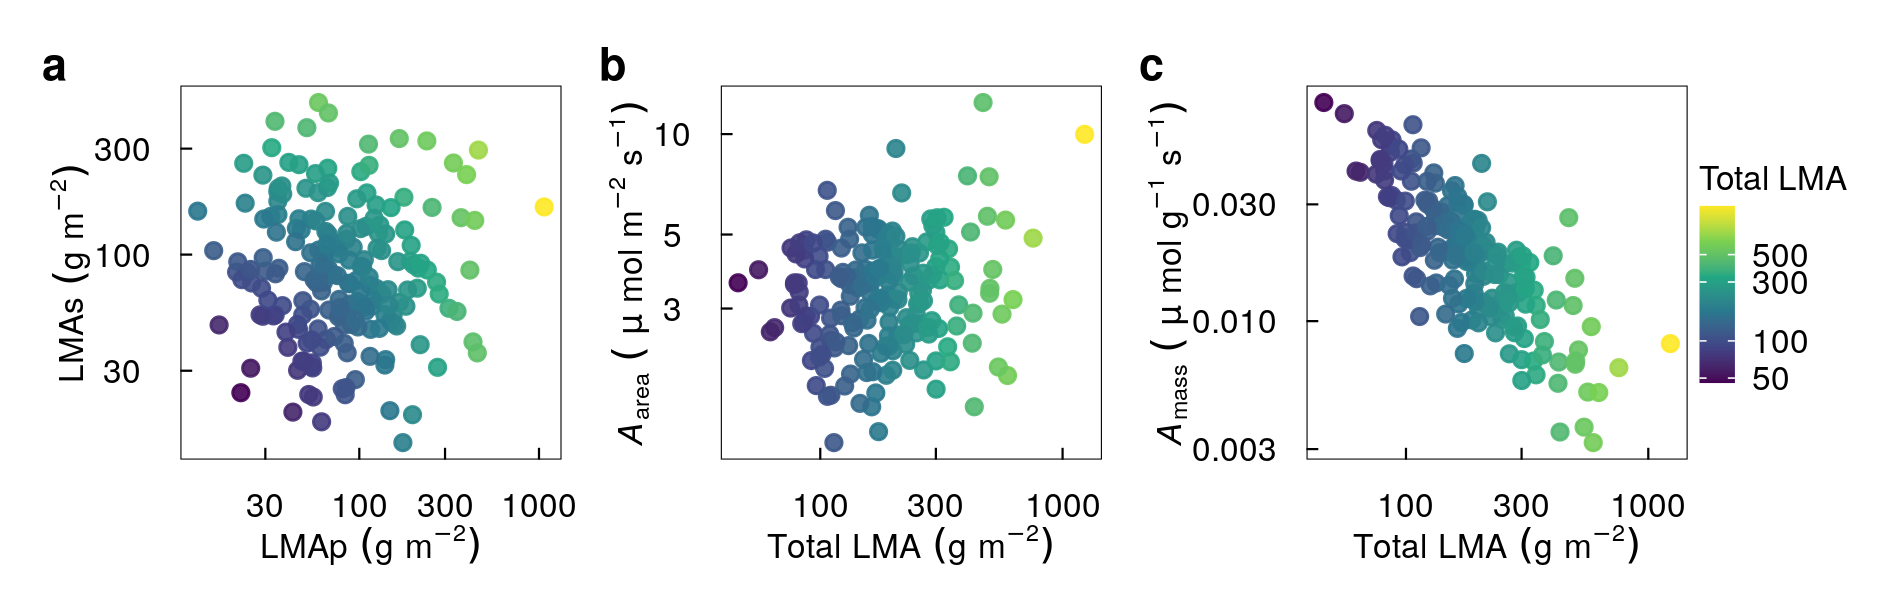
\includegraphics{/workspaces/LMAms/figs/hypo.png}

}

\caption{\label{fig-hypo}Simulated two-dimensional functional space that
can result in either a two- or one-dimensional trait space, depending on
how metabolic traits are normalized. (a) Hypothetical independent
variation in two leaf mass per area (LMA) components: metabolic leaf
mass per area (LMAm, which largely determines per-area values of
photosynthesis, respiration, and nutrient concentrations) and structural
leaf mass per area (LMAs, which determines leaf toughness but has little
effect on metabolic traits). Panels b and c represent normalization by
leaf area and leaf mass, respectively. (b) Two-dimensional relationship
between photosynthetic capacity (\emph{A}\textsubscript{max}) per-unit
leaf area and total LMA (equal to LMAm + LMAs). (c) One-dimensional
relationship between \emph{A}\textsubscript{max} per-unit leaf mass and
total LMA. Methods used to simulate the data are explained in Appendix
\DIFdelbeginFL \DIFdelFL{S3.}\DIFdelendFL \DIFaddbeginFL \DIFaddFL{S8}\DIFaddendFL }

\end{figure}%

\DIFaddbegin \newpage

\DIFaddend \begin{figure}

\centering{

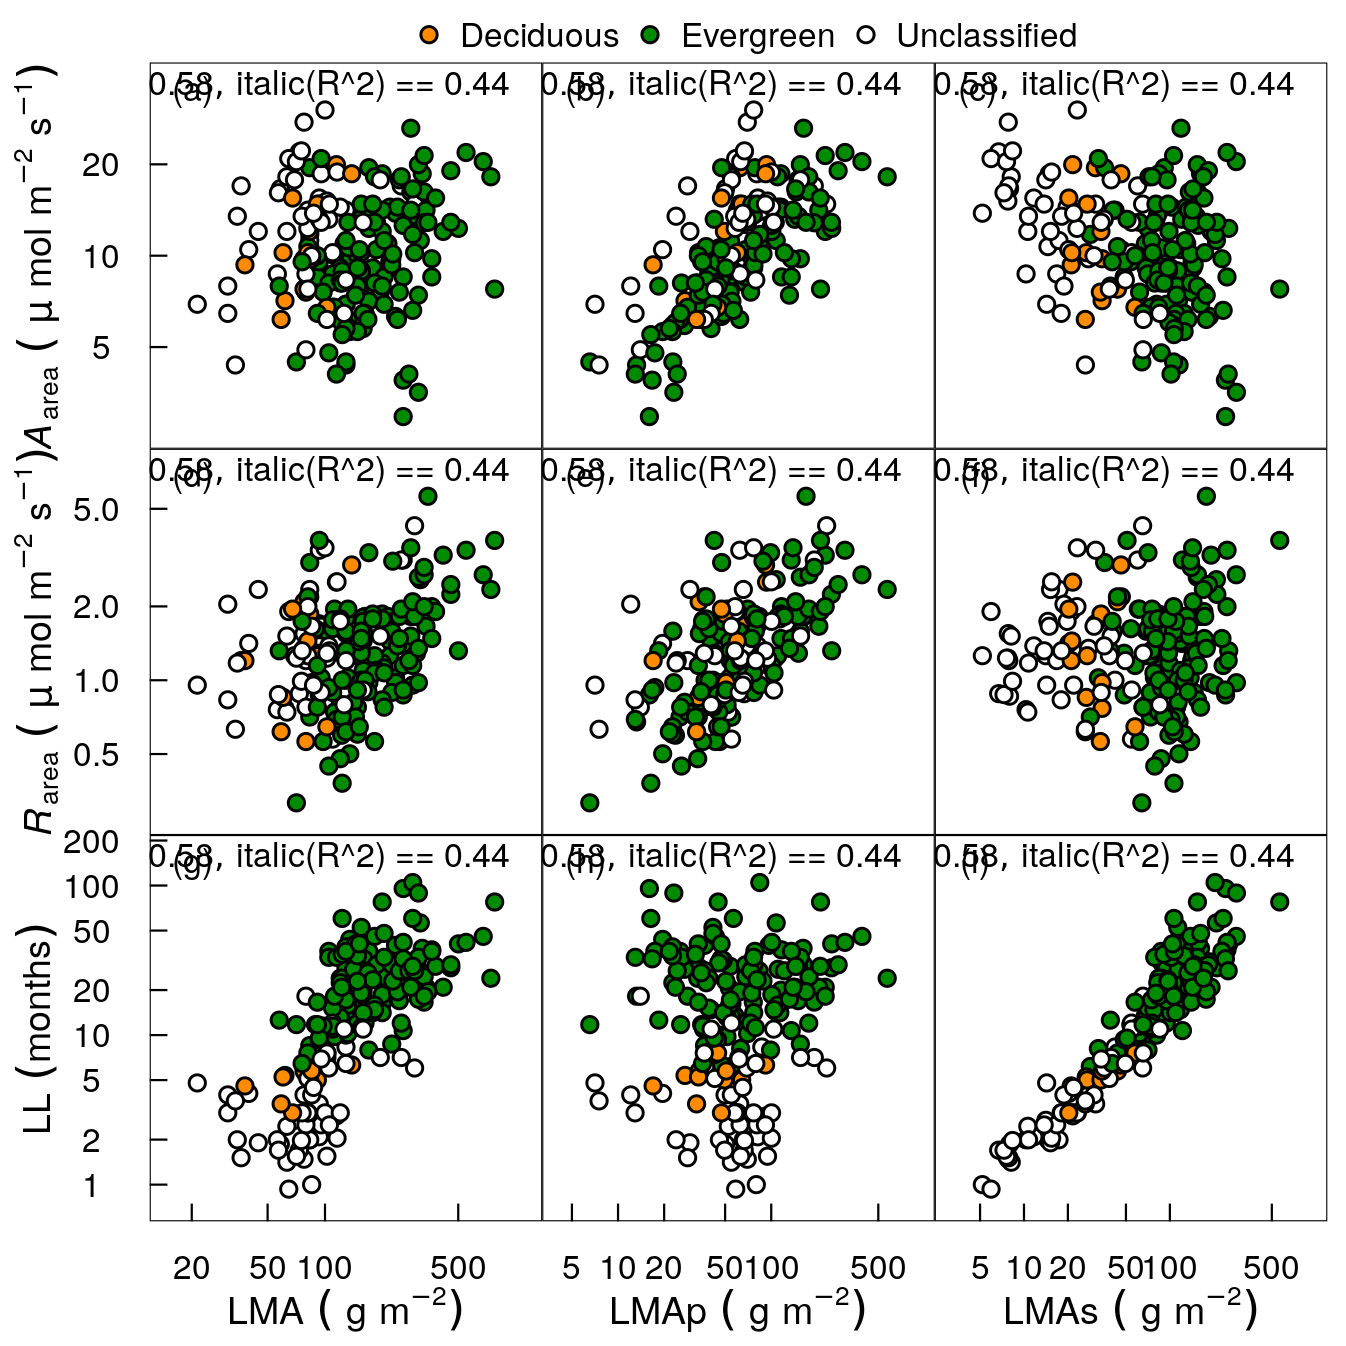
\includegraphics{/workspaces/LMAms/figs/gl_point.png}

}

\caption{\label{fig-gl_point}Observed and estimated leaf-trait
relationships in the global GLOPNET dataset. Estimates are from the best
GLOPNET model (Table 1). Leaf life span (LL), net photosynthetic rate
per unit leaf area (\emph{A}\textsubscript{area}), and dark respiration
rate per unit leaf area (\emph{R}\textsubscript{area}) are plotted
against observed LMA, posterior medians of LMAm and LMAs. Pearson
correlation coefficients (\emph{r}) for LMA (left column) and posterior
medians of Pearson correlation coefficients (\(\bar{r}\)) or partial
correlation coefficients (\(\bar{\rho}\)) for LMAm (middle column) and
LMAs (right column) are shown. Note that LL was modeled by LMAs alone
due to improved model performance with this parameter constraint (Table
1). Therefore, (\(\bar{r}\)) is reported for LL (single predictor
variable), whereas (\(\bar{\rho}\)) is reported for
\emph{A}\textsubscript{area} and \emph{R}\textsubscript{area} (multiple
predictor variables).}

\end{figure}%

\newpage

\begin{figure}

\centering{

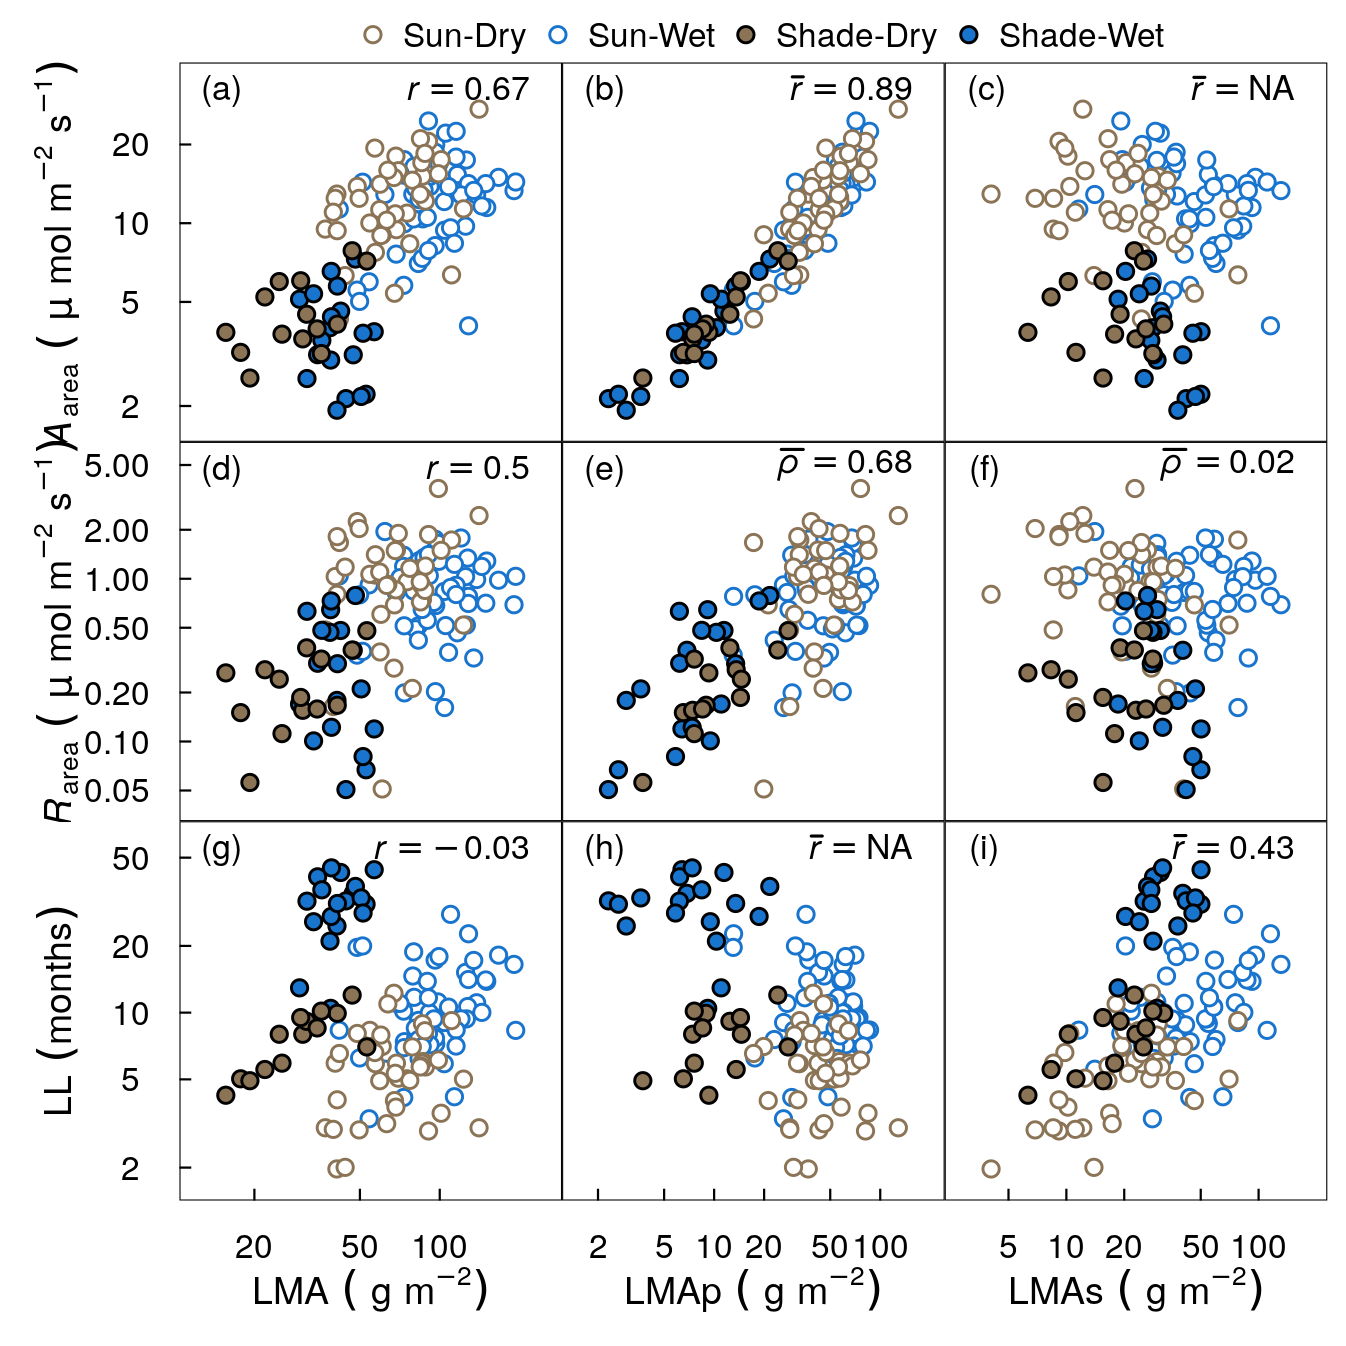
\includegraphics{/workspaces/LMAms/figs/pa_point.png}

}

\caption{\label{fig-pa_point}Observed and estimated leaf-trait
relationships in the Panama dataset. Estimates are from the best Panama
model (Table 1), which included effects of light on LL. Details as for
Fig.~\ref{fig-gl_point}. Note that \emph{A}\textsubscript{area} and LL
were modeled by LMAm and LMAs alone, respectively, due to improved model
performance with these parameter constraints (Table 1). The results
shown here include all leaves in the Panama dataset. The observed
separation of LL between sun and shade leaves is accounted for in the
model predictions Fig.~\ref{fig-ll_point}.}

\end{figure}%

\newpage

\begin{figure}

\centering{

\includegraphics{/workspaces/LMAms/figs/pa_point_par_ll.png}

}

\caption{\label{fig-ll_point}Relationship between leaf lifespan (LL) and
LMAs in the Panama dataset, after accounting for the effects of light
(suv vs.~shade leaves; see Eq. 4b). The dashed line indicates the 1:1
relationship expected for residuals on the log-scale. The posterior
medians of the partial correlation coefficient (\(\bar{\rho}\)) is
shown. The results shown here include all leaves in the Panama dataset.}

\end{figure}%

\newpage

\begin{figure}

\centering{

\includegraphics{/workspaces/LMAms/figs/vpart_intra.png}

}

\caption{\label{fig-vpart}Variance partitioning on LMA components
between and within leaf habits (evergreen vs.~deciduous) for the GLOPNET
dataset and the Panama dataset, and between and within sites (wet
vs.~dry) and light (sun vs.~shade) for the Panama dataset. To isolate
the effects of intraspecific variation, the Panama results shown here
only include species for which both sun and shade leaves were
available.}

\end{figure}%

\newpage

\begin{figure}

\centering{

\includegraphics{/workspaces/LMAms/figs/box_de.png}

}

\caption{\label{fig-box_de}Boxplots comparing leaf mass per area (LMA)
and posterior medians of photosynthetic and structural LMA components
(LMAm and LMAs, respectively) across deciduous (Dev) and evergreen (Eve)
leaves in the GLOPNET dataset (a) and in the Panama dataset (b). The
center line in each box indicates the median, upper and lower box edges
indicate the interquartile range, whiskers show 1.5 times the
interquartile range, and points are outliers. Groups sharing the same
letters are not significantly different (P \textgreater{} 0.05;
t-tests). The Panama results only include species for which both sun and
shade leaves were available. Qualitatively similar results were obtained
when all Panama species were included (Fig. S1). Note that the vertical
axis is on a log\textsubscript{10} scale.}

\end{figure}%

\newpage

\begin{figure}

\centering{

\includegraphics{/workspaces/LMAms/figs/box_pa.png}

}

\caption{\label{fig-box_pa}Boxplots comparing leaf mass per area (LMA)
and posterior medians of metabolic and structural LMA components (LMAm
and LMAs, respectively) across sites (wet and dry) and canopy strata
(sun and shade) in the Panama dataset. These results only include
species for which both sun and shade leaves were available.
Qualitatively similar results were obtained when all Panama species were
included (Fig. S1). Details as for Fig.~\ref{fig-box_de}.}

\end{figure}%

\newpage

\begin{figure}

\DIFdelbeginFL %DIFDELCMD < \centering{
%DIFDELCMD < 

%DIFDELCMD < 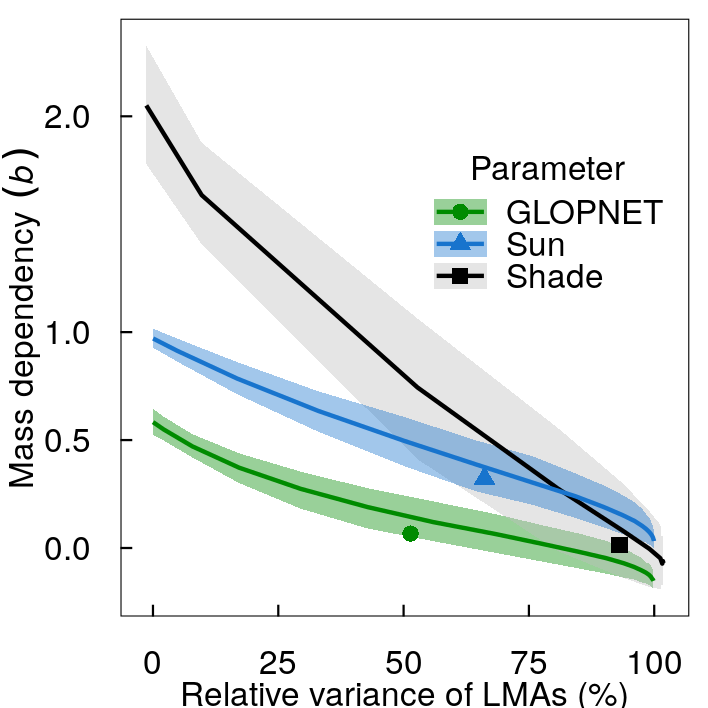
\includegraphics{/workspaces/LMAms/figs/mass_prop_mv.png}
%DIFDELCMD < 

%DIFDELCMD < }
%DIFDELCMD < %%%
\DIFdelendFL \DIFaddbeginFL \centering{

\captionsetup{labelsep=none}Relationships between mass dependency
(\emph{b} in Eq. S5) and LMAs variance (relative to total LMA variance;
Eq. S7) for the global GLPNET dataset, sun leaves in Panama, and shade
leaves in Panama. Solid lines indicate simulated medians and shaded
regions indicate 95\% confidence intervals. Each point indicates the
estimated values from the empirical data and represents interspecific
variation (e.g., across species within a canopy position in the Panama
dataset). The y-axis values indicates if photosynthetic capacity
(\emph{A}\textsubscript{max}) is is primarily mass-dependent (\emph{b}
\textgreater{} 0.5) or primarily area-dependent (0.5 \textgreater{}
\emph{b} \textgreater{} 0), with \emph{b} near 0 indicating purely
area-dependendence (\citeproc{ref-Osnas2018}{Osnas et al., 2018}). If
\emph{b} \textgreater{} 1, then \emph{A}\textsubscript{max} increases
exponentially with LMA, which is not consistent with observed
relationships (\citeproc{ref-Osnas2018}{Osnas et al., 2018}). See
Appendices S9-S6 for details.
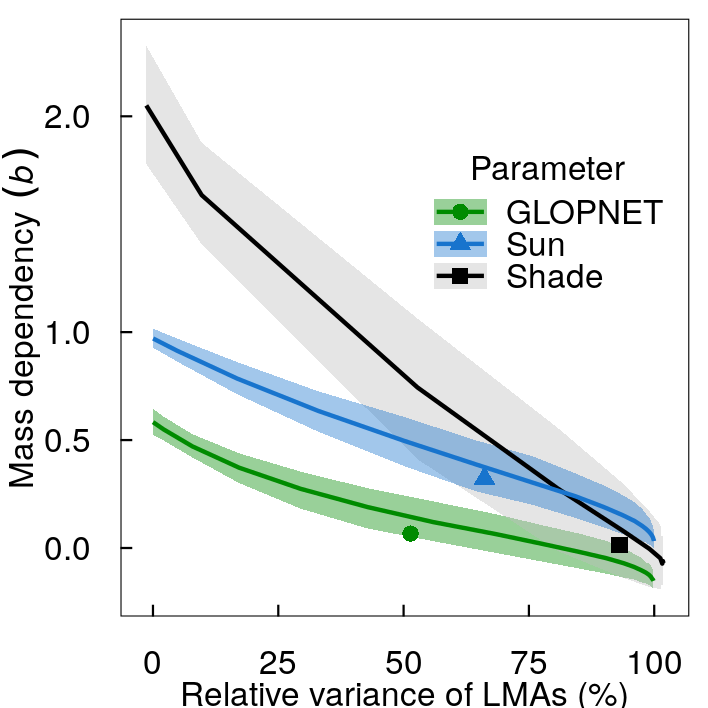
\includegraphics{/workspaces/LMAms/figs/mass_prop_mv.png}

}
\DIFaddendFL 

\caption{\label{fig-mass_prop}\DIFdelbeginFL \DIFdelFL{Relationships between mass dependency
(}\emph{\DIFdelFL{b}} %DIFAUXCMD
\DIFdelFL{in Eq. 5) and LMAs variance (relative to total LMA variance;
Eq. 6) for the global GLPNET dataset, sun leaves in Panama, and shade
leaves in Panama. Solid lines indicate simulated medians and shaded
regions indicate 95\% confidence intervals. Each point indicates the
estimated values from the empirical data and represents interspecific
variation (e.g., across species within a canopy position in the Panama
dataset). The y-axis values indicates if photosynthetic capacity
(}\emph{\DIFdelFL{A}}%DIFAUXCMD
\DIFdelFL{\textsubscript{max}) is is primarily mass-dependent (}\emph{\DIFdelFL{b}}
%DIFAUXCMD
\DIFdelFL{\textgreater{} 0.5) or primarily area-dependent (0.5 \textgreater{}
}\emph{\DIFdelFL{b}} %DIFAUXCMD
\DIFdelFL{\textgreater{} 0), with }\emph{\DIFdelFL{b}} %DIFAUXCMD
\DIFdelFL{near 0 indicating purely
area-dependendence (\mbox{%DIFAUXCMD
\citeproc{ref-Osnas2018}{Osnas et al. 2018}}\hspace{0pt}%DIFAUXCMD
). If
}\emph{\DIFdelFL{b}} %DIFAUXCMD
\DIFdelFL{\textgreater{} 1, then }\emph{\DIFdelFL{A}}%DIFAUXCMD
\DIFdelFL{\textsubscript{max} increases
exponentially with LMA, which is not consistent with observed
relationships (\mbox{%DIFAUXCMD
\citeproc{ref-Osnas2018}{Osnas et al. 2018}}\hspace{0pt}%DIFAUXCMD
).}\DIFdelendFL }

\end{figure}%

\newpage

\begin{figure}

\centering{

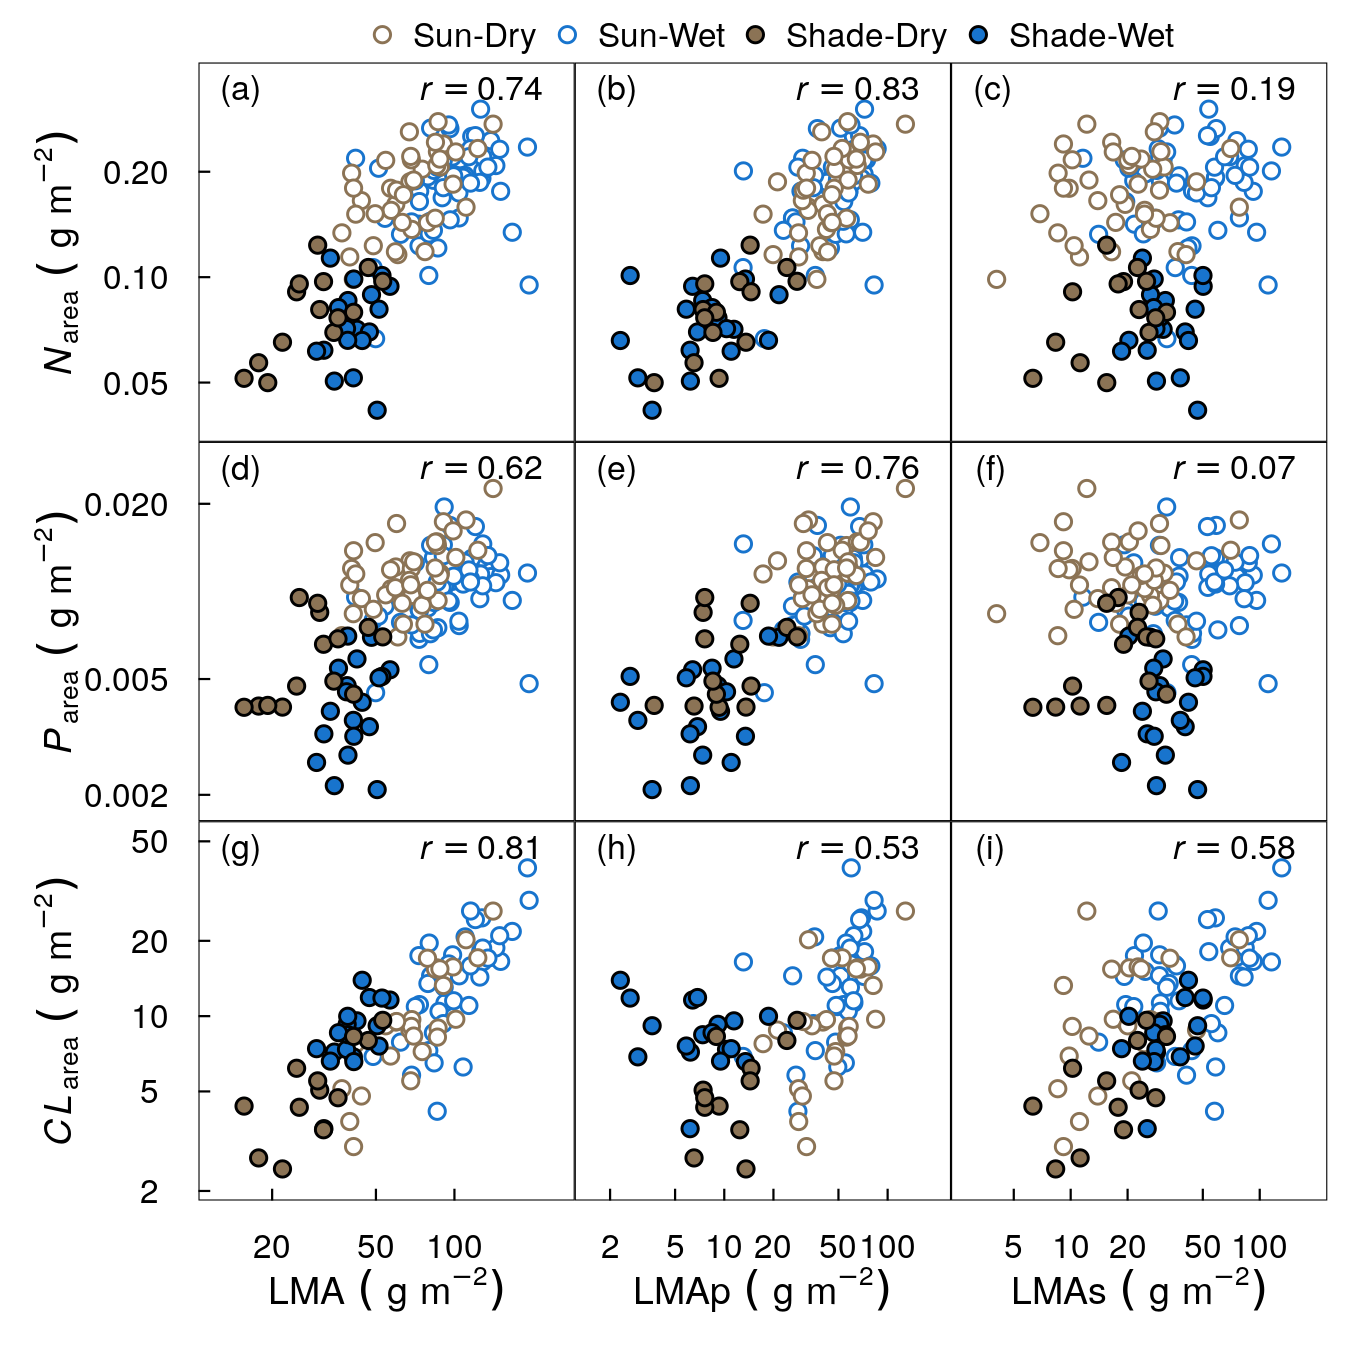
\includegraphics{/workspaces/LMAms/figs/pa_point_npc.png}

}

\caption{\label{fig-pa_npc}Measured traits in the Panama dataset related
to photosynthesis and metabolism (nitrogen and phosphorus per-unit leaf
area; \emph{N}\textsubscript{area} and \emph{P}\textsubscript{area}) are
better correlated with estimates (posterior medians) of the metabolic
LMA component (LMAm) than the structural component (LMAs), whereas the
opposite pattern occurs for a measured structural trait (cellulose
per-unit leaf area; CL\textsubscript{area}).
\emph{N}\textsubscript{area}, \emph{P}\textsubscript{area}, and
CL\textsubscript{area} data were not used to fit the models, and are
presented here as independent support for the model results. Pearson
correlation coefficients (\emph{r}) for LMA and the posterior medians of
Pearson correlation coefficients (\(\bar{r}\)) for LMAm and LMAs are
shown. Analogous results were obtained for \emph{N}\textsubscript{area}
and \emph{P}\textsubscript{area} for GLOPNET (Fig. S6). The results
shown here include all leaves for which \emph{N}\textsubscript{area},
\emph{P}\textsubscript{area} and CL\textsubscript{area} are available.}

\end{figure}%



\end{document}
